\documentclass[a4paper, twoside, 12pt, openright]{report}

\usepackage{booktabs}
\usepackage{verbatim}
\usepackage{graphicx}
\usepackage{float}
\usepackage{xcolor}
\usepackage{listings}
\usepackage{microtype}

\usepackage[english]{babel}
\usepackage{fancyhdr}
\usepackage{etoolbox}
\usepackage{geometry}
\usepackage{hyperref}
\usepackage{setspace}
\usepackage{titlesec}
\usepackage{newtxtext,newtxmath}
\usepackage[nottoc, numbib]{tocbibind}
\usepackage[nonumberlist, toc]{glossaries}
\usepackage[style=ieee, backend=biber]{biblatex}
\addbibresource{references.bib}

\newglossaryentry{api_rest}{
    name={REST API},
    description={Application Programming Interface based on the \textit{Representational State Transfer} (REST) paradigm, which uses the HTTP protocol to facilitate communication between systems and allows performing operations such as querying, creating, modifying and deleting resources in a scalable and efficient manner}
}

\newglossaryentry{gitops}{
    name={GitOps},
    description={Operational paradigm that uses Git repositories as the single source of truth for defining and managing the desired state of infrastructure and applications. Any change to the system is made through commits in the repository, and an automated operator (such as ArgoCD) is responsible for synchronising the actual state of the environment with the state declared in Git}
}

\newglossaryentry{cni}{
    name={CNI},
    description={(\textit{Container Network Interface}) Specification and set of libraries that define how network plugins should configure network interfaces of containers in Kubernetes. Examples of CNI plugins are Calico, Flannel and Cilium}
}

\newglossaryentry{drift_protection}{
    name={Drift protection},
    description={Mechanism that automatically detects and corrects any deviation between the desired state of a resource (defined declaratively) and its actual state in the system. In the context of Kyverno, it is implemented through the \texttt{synchronize: true} field in \textit{generate} policies, which automatically regenerates resources that are deleted or modified in an unauthorised manner}
}

\newglossaryentry{auto_hardening}{
    name={Auto-hardening},
    description={Automatic process of applying security configurations to system resources without manual intervention from the operator or developer. In the context of this work, it is implemented through Kyverno mutation policies that inject security fields into Kubernetes manifests at deployment time}
}

\newglossaryentry{imds}{
    name={IMDS},
    description={(\textit{Instance Metadata Service}) Service available in cloud environments (AWS, GCP, Azure) accessible from any instance through the link-local IP address \texttt{169.254.169.254}. It exposes sensitive instance information such as temporary IAM credentials, service tokens and network configuration. It is a common attack vector in compromised container environments}
}

\newglossaryentry{supply_chain_attack}{
    name={Supply chain attack},
    description={Type of attack that compromises the software or tools used during the development or deployment process, rather than directly attacking the target system. In CI/CD environments, it can manifest as the manipulation of dependencies, container images, GitHub Actions or third-party runners to inject malicious code into the pipeline}
}

\newglossaryentry{policy_report}{
    name={PolicyReport},
    description={Native Kubernetes resource automatically generated by Kyverno that consolidates the results of policy evaluation over cluster resources. It indicates which resources have passed, failed or been mutated by each policy, with a timestamp for each evaluation. There are two variants: \texttt{PolicyReport} (namespace-scoped) and \texttt{ClusterPolicyReport} (cluster-scoped)}
}

\newglossaryentry{webhook}{
    name={Webhook},
    description={Kubernetes API Server extension mechanism that allows invoking external HTTP services during the resource admission process. In the context of Kyverno, admission webhooks are the channel through which the API Server delegates policy evaluation to the Kyverno engine. There are two types: \texttt{MutatingWebhookConfiguration} (for mutation policies) and \texttt{ValidatingWebhookConfiguration} (for validation policies)}
}

\newglossaryentry{etcd}{
    name={etcd},
    description={Distributed key-value database that acts as the persistent store for the complete Kubernetes cluster state. All cluster objects (pods, services, configmaps, policies, etc.) are persisted in etcd once the admission process has been passed. Its consistency and availability are critical for cluster operation}
}

\newglossaryentry{hardening}{
    name={Hardening},
    description={Process of reducing the attack surface of a system by eliminating or restrictively configuring unnecessary functionalities. In the context of Kubernetes containers, it includes measures such as disabling privilege escalation, removing unneeded Linux capabilities, enforcing execution as a non-root user and restricting filesystem access}
}

\newglossaryentry{cidr}{
    name={CIDR},
    description={(\textit{Classless Inter-Domain Routing}) Notation used to define IP address ranges. In Kubernetes, CIDR ranges are used to designate the pod address space (pod CIDR) and service address space (service CIDR). For example, \texttt{10.244.0.0/16} defines the range of IPs assignable to pods when using Calico as the CNI plugin}
}

\newglossaryentry{two_repo_gitops}{
    name={Two-repository pattern (GitOps)},
    description={GitOps architectural pattern that separates the application source code repository from the configuration repository containing Kubernetes manifests. The CI pipeline updates the configuration repository after a successful build, and ArgoCD synchronises the cluster with the state declared in that repository. This separation improves security by limiting cluster access permissions and clarifies the responsibilities of each component}
}

\newglossaryentry{qos_kubernetes}{
    name={QoS (Kubernetes)},
    description={(\textit{Quality of Service}) Classification that Kubernetes assigns to pods based on how their \texttt{resources.requests} and \texttt{resources.limits} are defined. There are three classes: \texttt{Guaranteed} (requests == limits for all containers --- maximum protection against eviction), \texttt{Burstable} (requests < limits or only one defined) and \texttt{BestEffort} (no fields defined --- first class to be evicted under resource pressure)}
}

\newglossaryentry{patchstrategicmerge}{
    name={patchStrategicMerge},
    description={Kyverno patch application mechanism that performs an intelligent merge (\textit{merge}) of the original Kubernetes object with the patch defined in the policy. Unlike a complete replacement, \texttt{patchStrategicMerge} only adds absent fields and respects values already explicitly declared in the original manifest, guaranteeing that mutations are additive and non-destructive}
}

\newglossaryentry{runner}{
    name={Runner (GitHub Actions)},
    description={Execution agent that processes jobs defined in GitHub Actions workflows. It can be a GitHub-hosted runner (\textit{hosted runner}) or a self-managed runner on own infrastructure (\textit{self-hosted runner}). Runners execute each pipeline step in an isolated environment and are the target of supply chain attacks that seek to compromise the build process or exfiltrate CI environment credentials}
}

\newglossaryentry{multi_tenant}{
    name={Multi-tenant},
    description={Kubernetes deployment model in which a single cluster is shared by multiple teams, applications or clients (called \textit{tenants}) with logical isolation through namespaces, RBAC and Network Policies. This model optimises resource usage but introduces security challenges related to tenant isolation, especially in scenarios where a workload compromise could propagate to others}
}


\setglossarystyle{altlist}
\setacronymstyle{long-short}

\makeglossaries

% ── Style for code blocks, commands and YAML manifests ────────────────────────
\definecolor{codbg}{RGB}{247,247,247}
\definecolor{codborder}{RGB}{210,210,210}
\lstdefinestyle{tfmcode}{
  backgroundcolor  = \color{codbg},
  basicstyle       = \ttfamily\small,
  breaklines       = true,
  breakatwhitespace= false,
  postbreak        = \mbox{{\footnotesize$\hookrightarrow$}\space},
  frame            = single,
  rulecolor        = \color{codborder},
  framesep         = 5pt,
  xleftmargin      = 8pt,
  xrightmargin     = 8pt,
  keepspaces       = true,
  columns          = flexible,
  showstringspaces = false,
  tabsize          = 2,
  aboveskip        = 4pt,
  belowskip        = 4pt,
  literate =
    {á}{{\'{a}}}1 {é}{{\'{e}}}1 {í}{{\'{i}}}1 {ó}{{\'{o}}}1 {ú}{{\'{u}}}1
    {Á}{{\'{A}}}1 {É}{{\'{E}}}1 {Í}{{\'{I}}}1 {Ó}{{\'{O}}}1 {Ú}{{\'{U}}}1
    {ñ}{{\~{n}}}1 {Ñ}{{\~{N}}}1
}
\lstset{style=tfmcode}
% ────────────────────────────────────────────────────────────────────────────

\titleformat{\chapter}[block]{\normalfont\fontsize{18pt}{0pt}\bfseries}{\thechapter}{1em}{}
\titlespacing*{\chapter}{0pt}{0pt}{\baselineskip}
\titlespacing*{\section}{0pt}{1.5ex plus .2ex}{0.8ex}
\titlespacing*{\subsection}{0pt}{1.5ex plus .2ex}{0.8ex}

\titleformat{\section}[block]{\normalfont\fontsize{16pt}{0pt}\bfseries}{\thesection}{1em}{}
\titleformat{\subsection}[block]{\normalfont\fontsize{14pt}{0pt}\bfseries}{\thesubsection}{1em}{}

\hypersetup{
    colorlinks=true,
    linkcolor=black,
    citecolor=black,
    filecolor=magenta,
    urlcolor=blue,
    pdftitle={Master's Thesis},
    pdfauthor={Ziad El Karrabi El Hanafi},
    pdfpagemode=FullScreen
}

\geometry{top=3cm, bottom=2.54cm, left=2.54cm, right=2.54cm, bindingoffset=0.46cm}

\setlength{\headheight}{14.5pt}

\setlength{\parindent}{0pt}

\graphicspath{{images/}}

\fancypagestyle{plain}{
    \fancyhf{}
    \fancyhead[RO,LE]{\fontsize{10}{12}\textit{\thepage}}
    \fancyhead[RE]{\fontsize{10}{12}\textit{Master's Thesis}}
    \fancyfoot{}
}
\pagestyle{plain}

\title{
    \begin{center}
        \begin{minipage}{0.45\linewidth}
            \centering
            
\includegraphics[width=0.7\linewidth]{images/logo-tecnocampus.png}
        \end{minipage}
        \hfill
        \begin{minipage}{0.45\linewidth}
            \centering
            
\includegraphics[width=0.35\linewidth]{images/logo-udg.png}
        \end{minipage}

        \vspace{1.5cm}

        {\fontsize{14pt}{0pt}\textbf{Applied Computer Security to Industrial Environments}} \\[1cm]

        \textbf{Design and implementation of a DevSecOps architecture based on GitOps:}\\
        \textbf{Supply chain security in Kubernetes using scanners, ArgoCD and Kyverno} \\[1.5cm]

        \textbf{Master's Thesis} \\[5cm]
    \end{center}
}
\author{
\fontsize{14pt}{0pt}
\textbf{Ziad El Karrabi El Hanafi} \\
\textbf{Supervisor: Josep Andreu}
}
\date{2026}

\fontsize{12pt}{0pt}
\begin{document}

\maketitle

\newpage
\thispagestyle{empty}
\null
\newpage

\pagenumbering{Roman}

\tableofcontents

\listoffigures

\listoftables

\onehalfspacing
\setlength{\parskip}{12pt}

\fancypagestyle{plain}{
    \fancyhf{}
    \fancyhead[RO,LE]{\fontsize{10}{12}\textit{\thepage}}
    \fancyhead[LO]{\fontsize{10}{12}\textit{\nouppercase{\textit{\leftmark}}}}
    \fancyhead[RE]{\fontsize{10}{12}\textit{Master's Thesis}}
    \fancyfoot{}
}
\pagestyle{plain}
\pagenumbering{arabic}
\chapter{Introduction}

The adoption of container-based architectures and orchestrators such as Kubernetes has transformed how applications are developed and deployed in cloud and enterprise environments. This paradigm enables automated lifecycle management of applications, improves scalability and facilitates the integration of modern development practices. However, this technological evolution also introduces new security challenges, especially in environments where deployments are carried out in an automated and continuous manner.

In this context, the DevSecOps approach has emerged, with the objective of integrating security within the software development lifecycle itself, rather than treating it as a post-deployment phase. This model promotes the automation of security controls within continuous integration and deployment pipelines, enabling the detection of vulnerabilities, the application of security policies and the guarantee of secure configurations from the earliest stages of development.

This Master's Thesis focuses on the implementation of a complete DevSecOps environment on Kubernetes, integrating Continuous Integration tools (GitHub Actions) with automated vulnerability analysis using tools such as Trivy and Sysdig Secure. A GitOps-based Continuous Deployment model using ArgoCD is also implemented, enabling the declarative management of infrastructure and deployments through Git repositories.

Additionally, Kyverno is incorporated as a Policy-as-Code security policy engine, enabling the automatic enforcement of controls over Kubernetes manifests during the deployment process.

The core of the project is based on the use of Admission Controllers, specifically Kyverno, to apply security policies declaratively within the Kubernetes cluster. Unlike traditional approaches that only block insecure configurations, this work explores the use of mutating policies, capable of automatically correcting insecure configurations in YAML manifests at deployment time.

Finally, the project includes a comparative analysis between Kyverno and OPA Gatekeeper, evaluating their capabilities in implementing security policies in Kubernetes, their ease of use, learning curve and effectiveness in production environments.

Figure~\ref{fig:arquitectura-devsecops} shows a general overview of the DevSecOps architecture implemented in this work, where development processes, security analysis, continuous deployment and policy enforcement are all integrated within a Kubernetes environment.

\begin{figure}[H]
\centering
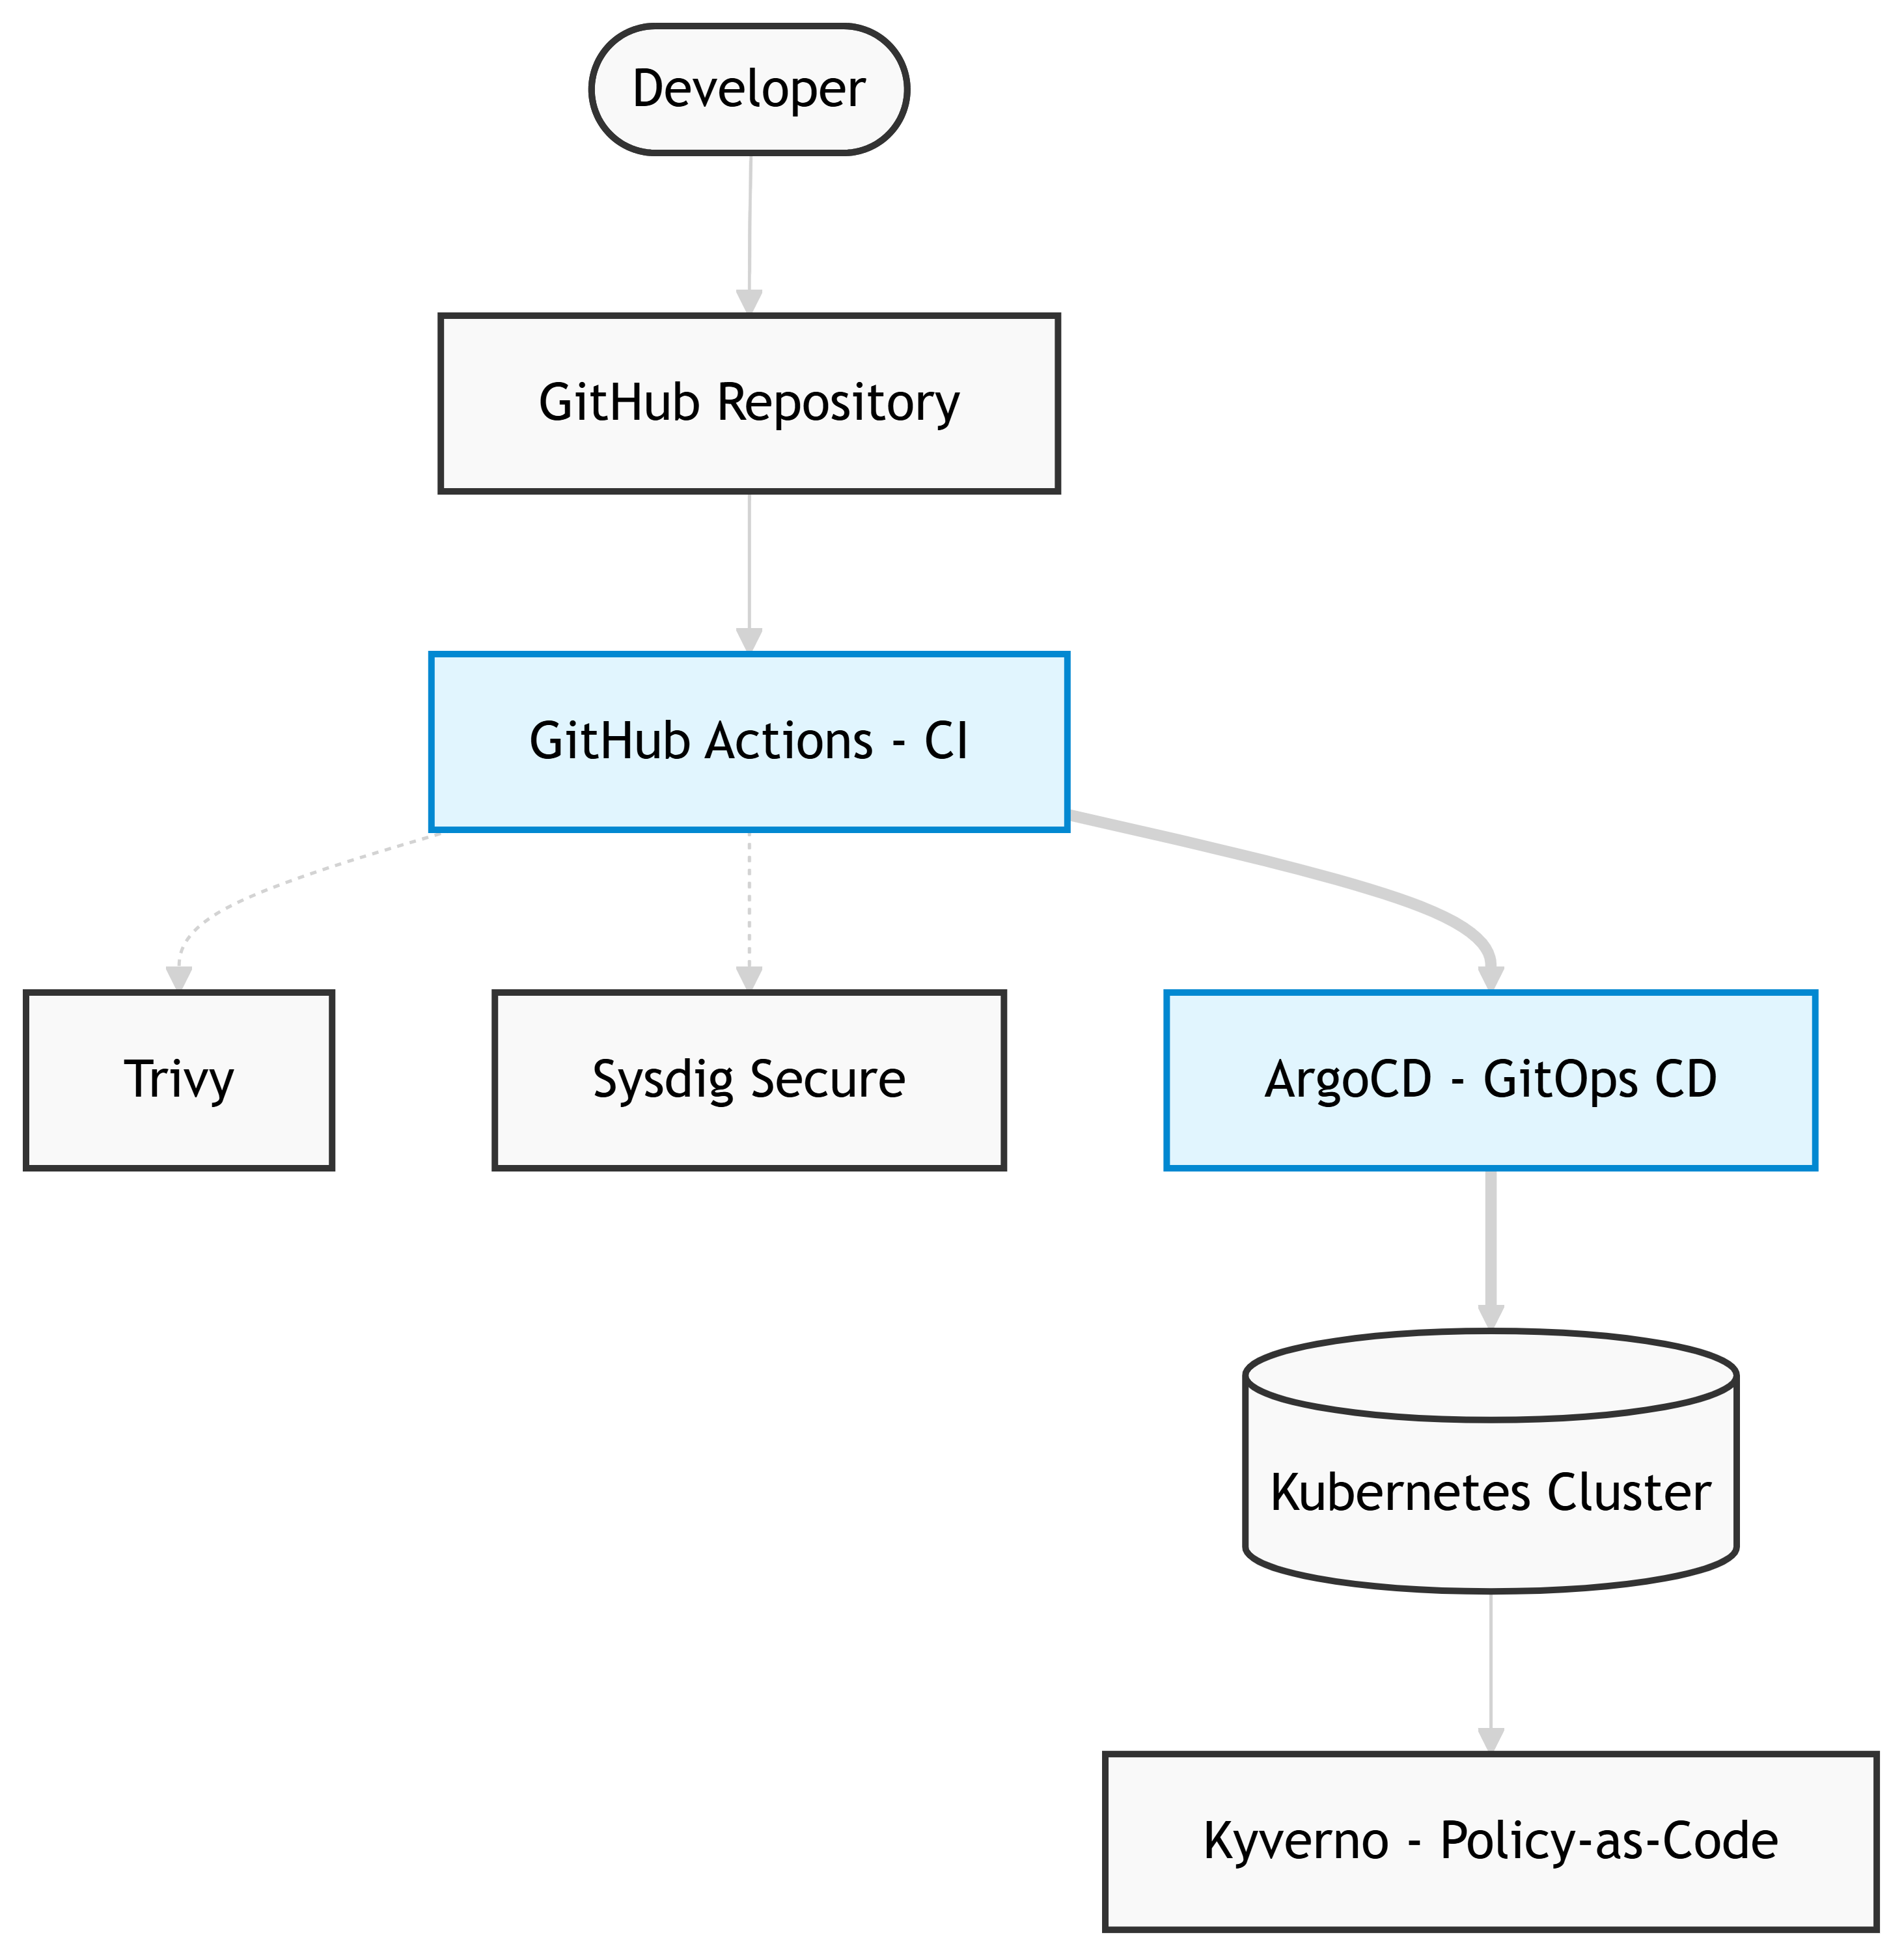
\includegraphics[width=0.5\linewidth]{images/arquitectura_DevSecOps.png}
\caption{General architecture of the DevSecOps environment}
\label{fig:arquitectura-devsecops}
\end{figure}

\chapter{Theoretical Framework and Reference Analysis}

\section{Evolution from the DevOps to the DevSecOps paradigm}

\subsection{Limitations of traditional models}

Traditional software development models, such as the waterfall model, are characterised by a strict separation of phases (analysis, development, testing and deployment), which hinders the early detection of errors and vulnerabilities \cite{pressman2019software}. In these approaches, security is usually introduced in the final stages, significantly increasing the cost of correction and the risk in production.

The adoption of agile methodologies and, subsequently, the DevOps paradigm improved collaboration between teams and accelerated delivery cycles \cite{kim2016devops}. However, various studies highlight that security continued to be treated as an independent process, generating vulnerabilities especially in cloud-native environments \cite{sharma2020devsecops}.

In this context, the need to integrate automated security mechanisms that can be applied continuously within the software lifecycle becomes evident.

\subsection{Integration of security in the software lifecycle}

The evolution towards DevSecOps implies integrating security from the earliest phases of development, incorporating automated controls in CI/CD pipelines \cite{behl2017devsecops}. This includes vulnerability analysis, configuration validation and compliance control.

Automation enables consistency and reduces human errors, especially in dynamic environments. According to \cite{rahman2019devsecops}, the early integration of security significantly improves software resilience.

This approach is key in the present work, where security is implemented through automated mechanisms integrated in Kubernetes.

\subsection{Birth of the DevSecOps concept}

DevSecOps emerged as a natural evolution of DevOps, integrating security as an intrinsic component of the software lifecycle \cite{mohan2016towards}. This paradigm promotes the automation of security controls and shared responsibility across teams.

In container and Kubernetes-based environments, this approach requires mechanisms capable of applying security policies dynamically and at scale.

In this work, this objective is materialised through the use of Policy-as-Code and tools such as Kyverno, which enable declarative and automated security enforcement.

\section{Kubernetes as an execution platform}

\subsection{Kubernetes architecture}

Kubernetes has consolidated itself as the de facto standard for container orchestration, providing a robust platform for the management of distributed applications \cite{burns2016borg}.

Its architecture is based on a control plane, which manages the state of the system, and worker nodes responsible for running workloads. The API Server acts as the central interaction point through a declarative model \cite{kubernetes_docs}.

This architecture enables automated system management, but also introduces new security challenges that must be addressed through specific mechanisms.

\subsection{Main cluster components}

The main control plane components include the API Server, the Scheduler and the Controller Manager, responsible for processing requests and maintaining the desired state of the system. On worker nodes, the kubelet and the container runtime enable the execution of pods \cite{kubernetes_docs}.

The existence of multiple distributed components makes it necessary to implement centralised security controls, such as Admission Controllers.

\subsection{Network management and Network Policies}

By default, Kubernetes allows free communication between pods, which can represent a significant risk. Network Policies allow defining communication rules based on labels and namespaces, applying the principle of least privilege \cite{kubernetes_docs}.

Furthermore, in real environments it is common to find insecure configurations such as:

\begin{itemize}
\item Containers running as the root user
\item Privilege escalation enabled
\item Missing resource limits
\item Unrestricted network access
\end{itemize}

These practices pose a high risk, especially in \textit{multi-tenant} environments ---where multiple teams, applications or clients share a single Kubernetes cluster with logical isolation via namespaces--- since a compromise in one workload can propagate to others if there are no adequate network, execution and privilege controls.

This justifies the need to apply automatic controls at deployment time through Kubernetes security policies.

\section{Policy-as-Code and Admission Controllers}

\subsection{How Admission Controllers work}

Admission Controllers are API Server mechanisms that intercept requests before resources are deployed in the cluster \cite{kubernetes_docs}. They allow applying validations or modifications to objects.

This mechanism constitutes the technical basis on which security is implemented in this work.

\subsection{Resource validation vs. mutation}

\textit{Validating admission controllers} allow verifying that resources comply with certain policies, rejecting those that do not satisfy them.

On the other hand, \textit{mutating admission controllers} allow automatically modifying resources before their creation, applying secure default configurations.

In this work, special emphasis is placed on \textit{mutating} policies, as they enable automatic hardening mechanisms to be applied to manifests, correcting insecure configurations without user intervention.

This approach is key to ensuring security in highly automated DevSecOps environments.

\subsection{Importance of declarative security}

The Policy-as-Code approach allows defining security policies as versioned code, facilitating their integration into GitOps workflows \cite{huttermann2022devops}.

This model improves traceability, reproducibility and automation of security.

In this work, these mechanisms are implemented using Kyverno to automatically apply policies at deployment time.

\section{Tools and technologies used}

\subsection{Kyverno}

Kyverno is a Policy-as-Code tool designed specifically for Kubernetes that allows defining policies using YAML, without the need to learn additional languages \cite{kyverno_docs}.

Unlike other solutions, Kyverno allows defining policies directly in the same format used by Kubernetes, which facilitates its adoption. Furthermore, it supports both validation and mutation policies, enabling not only the blocking of insecure configurations but also their automatic correction.

This capability is especially relevant in DevSecOps environments, where automation and consistency are key factors.

Kyverno constitutes the central axis of this work.

\subsection{OPA Gatekeeper}

Open Policy Agent (OPA) is a general-purpose policy engine that allows defining rules using the Rego language \cite{opa_docs}. Gatekeeper facilitates its integration with Kubernetes.

Although it offers great flexibility, its complexity and validation-focused approach differentiate it from Kyverno.

\subsection{ArgoCD and GitOps}

ArgoCD implements the GitOps paradigm, where the state of the system is defined in Git repositories \cite{weaveworks_gitops}.

In this work, it is used to automate deployment and ensure consistency between configuration and real state.

\subsection{GitHub Actions}

GitHub Actions enables the automation of CI/CD pipelines, including build, test and security processes \cite{github_actions_docs}.

It is used to integrate security controls within the DevSecOps workflow.

\subsection{Trivy and Sysdig Secure}

Trivy enables vulnerability scanning of container images \cite{trivy_docs}, while Sysdig Secure provides runtime security \cite{sysdig_secure}.

These tools complement the security applied through Kubernetes policies.

\section{Theoretical comparison: Kyverno vs OPA}

Kyverno and Open Policy Agent (OPA) represent two of the most relevant solutions within the \textit{Policy-as-Code} approach applied to Kubernetes. Both allow defining and applying security policies over cluster resources, although they present significant differences in terms of design, approach and capabilities \cite{opa_docs, kyverno_docs}.

Kyverno is a \textit{Kubernetes-native} tool that allows defining policies using the same YAML format used in the system's own manifests. This approach reduces complexity and facilitates adoption by DevOps teams familiar with Kubernetes. By contrast, OPA uses the Rego language, a general-purpose declarative language that offers great flexibility but introduces a steeper learning curve.

From a functional standpoint, both tools support the implementation of validation policies (\textit{validating}), that is, checking that resources meet certain conditions before being deployed. However, a key difference lies in the support for mutation policies (\textit{mutating}). Kyverno allows automatically modifying resources at admission time, applying secure default configurations, while OPA Gatekeeper focuses primarily on validation, lacking native support for resource mutation.

The following table presents a summarised comparison of both tools:

\begin{table}[H]
\centering
\begin{tabular}{lcc}
\toprule
\textbf{Feature} & \textbf{Kyverno} & \textbf{OPA Gatekeeper} \\
\midrule
Approach & Kubernetes-native & General-purpose \\
Policy language & YAML & Rego \\
Learning curve & Low & High \\
Resource validation & Yes & Yes \\
Resource mutation & Yes & No (limited) \\
Kubernetes integration & Native & Via CRDs \\
Ease of adoption & High & Medium \\
\bottomrule
\end{tabular}
\caption{Comparison between Kyverno and OPA Gatekeeper}
\label{tab:kyverno-vs-opa}
\end{table}


These differences have a direct impact on their applicability in DevSecOps environments. While OPA offers greater expressiveness and flexibility for defining complex policies, Kyverno stands out for its operational simplicity and its ability to integrate naturally into Kubernetes-based workflows.

From the perspective of this work, Kyverno's mutation capability is especially relevant, as it allows implementing automatic \textit{hardening} mechanisms over manifests, correcting insecure configurations without the need for manual intervention. This includes, for example, the automatic addition of resource limits, the disabling of elevated privileges or the application of default network policies.

Consequently, Kyverno is positioned as a tool especially suited for environments where automation, consistency and integration with GitOps practices are prioritised.

This theoretical comparison will serve as the basis for the practical analysis developed in later chapters, where the behaviour of both solutions will be evaluated in a real Kubernetes environment.

\chapter{Objectives and Scope}

\section{General objective}

The main objective of this Master's Thesis is the design and implementation of a functional DevSecOps environment on Kubernetes, integrating security mechanisms natively within the software development and deployment lifecycle.

The core of the project focuses on applying the Policy-as-Code paradigm through the use of Admission Controllers, specifically Kyverno, with the objective of guaranteeing secure configurations at deployment time. Unlike traditional approaches based solely on detection or blocking, this work places special emphasis on the use of \textit{mutating} policies, capable of automatically correcting insecure configurations in Kubernetes manifests.

This approach enables not only the prevention of configuration errors, but also the establishment of automatic hardening mechanisms aligned with modern security practices in cloud-native environments.

\section{Specific objectives}

To achieve the general objective, the following specific objectives are defined:

\begin{itemize}
    \item Deploy a functional Kubernetes cluster in a laboratory environment, with an architecture based on one control node and one worker node, properly configuring communication and the network layer via a CNI solution such as Calico.

    \item Install and configure Kyverno as a Policy-as-Code security policy engine, integrating it as an Admission Controller within the cluster.

    \item Define and implement a representative set of security policies (between 5 and 10), focused on real-world issues such as:
    \begin{itemize}
        \item containers running with elevated privileges,
        \item privilege escalation,
        \item absence of resource limits,
        \item unrestricted network communication.
    \end{itemize}

    \item Validate policy behaviour through practical tests, demonstrating both the blocking of insecure configurations (\textit{validating policies}) and their automatic correction (\textit{mutating policies}).

    \item Implement an advanced policy based on the automatic generation of Network Policies, with the objective of restricting access to sensitive resources, such as metadata services (for example, IP 169.254.169.254), common in cloud environments.

    \item Integrate the cluster within a GitOps-based continuous deployment model, using ArgoCD to manage the declarative state of applications.

    \item Incorporate a continuous integration pipeline via GitHub Actions, including build and vulnerability analysis processes with tools such as Trivy or Sysdig Secure.

    \item Perform a technical comparison between Kyverno and OPA Gatekeeper, analysing differences in ease of use, validation and mutation capabilities, and suitability in production environments.
\end{itemize}

\section{Project scope}

The project is developed in a laboratory environment based on virtual machines, with the objective of reproducing a realistic Kubernetes deployment scenario. The scope includes the cluster configuration, the integration of the main DevSecOps pipeline tools and the implementation of representative security policies.

However, the work does not aim to cover all existing security standards exhaustively, but rather to demonstrate the functionality and viability of the Policy-as-Code model applied to Kubernetes through practical case studies.

Additionally, the use of automation tools such as Ansible is considered a possible extension of the project. Following an iterative approach, priority is initially given to the implementation of security mechanisms and their validation, leaving the complete deployment automation as future or parallel work depending on available time.

\chapter{Project Methodology}

This chapter describes the methodological approach adopted to carry out the Master's Thesis. This is not a technical chapter, but rather a reasoned description of how the work has been planned, what decisions have been made regarding scope and project organisation, and what criteria have guided tool selection and the definition of development phases. Many of these decisions were agreed upon with the supervisor, Josep Andreu, through various meetings and communications that have progressively refined the approach of the work.

% ─────────────────────────────────────────────
\section{General project approach}
% ─────────────────────────────────────────────

The project adopts an approach of \textbf{applied research with practical development}. The objective is not to carry out an exhaustive theoretical review of Kubernetes security standards, but to build a real functional environment that demonstrates how to integrate security in an automated manner within the development and deployment lifecycle. Results are validated empirically through controlled tests on the implemented environment, not through bibliographic analysis.

The supervisor oriented the work towards a manageable number of between five and ten well-chosen security policies, with the argument that demonstrating the functioning and deep understanding of Kyverno is academically more valuable than applying a complete standard superficially. This guideline has shaped the entire project planning: quality and justification of each decision are prioritised over the quantity of elements implemented.

Development follows an \textbf{iterative and incremental} model: starting with the most fundamental components (the cluster and Kyverno), validating each element before adding the next, and progressively advancing towards components of greater complexity (ArgoCD, GitHub Actions, comparison with OPA). This model enables early detection of integration problems and guarantees that the environment is functional at all times, even before it is complete.

% ─────────────────────────────────────────────
\section{Laboratory environment}
% ─────────────────────────────────────────────

The environment on which the project is developed consists of a Kubernetes cluster deployed on two virtual machines provided by the supervisor, managed with VirtualBox. This decision was agreed upon during the initial exchange with Josep Andreu, who recommended using the virtual machine images used in the course subject to guarantee coherence and stability.

The two virtual machines have the following roles and fixed IP addresses within the laboratory network:

\begin{itemize}
    \item \textbf{Control node} (\textit{control plane}): \texttt{192.168.1.101}, hostname \texttt{control}. Hosts the Kubernetes control plane and acts as the entry point for all cluster administration operations.
    \item \textbf{Worker node}: \texttt{192.168.1.102}, hostname \texttt{worker}. Executes the workloads deployed in the cluster.
\end{itemize}

Each virtual machine is configured with two network interfaces: one NAT type for internet access, and one \textit{Host-only Adapter} type for internal communication between nodes. The cluster network layer is implemented using \textbf{Calico v3.28} \cite{calico_docs}, a CNI plugin that allows defining and effectively applying Network Policies, which is a requirement for one of the security policies implemented in the project.

The choice of a local virtualised environment, rather than a cloud provider, responds to criteria of control and reproducibility. However, this decision has implications for the project scope, which are detailed at the end of this chapter.

% ─────────────────────────────────────────────
\section{Project phases}
% ─────────────────────────────────────────────

The project is organised into five sequential phases. Each phase has a defined scope and the next phase is not started until the previous one has been verified as functional.

\subsection{Phase 1: Kubernetes cluster provisioning}

The first phase encompasses the setup of the Kubernetes cluster on the two laboratory virtual machines. It includes the initialisation of the control node, the joining of the worker node and the installation of the Calico network plugin. The expected result is an operational cluster with both nodes active and all system components running.

\subsection{Phase 2: Kyverno deployment and integration}

The second phase introduces Kyverno as the security policy engine within the cluster. Kyverno is installed as a set of controllers that integrate with Kubernetes' Admission Controllers mechanism, intercepting requests to the API Server to apply the defined policies. This phase also includes the verification that Kyverno's webhooks are correctly registered and operational before proceeding with policy implementation.

\subsection{Phase 3: Security policy implementation}

The third phase constitutes the core of the work. A set of security policies covering the three types of actions available in Kyverno is designed and implemented: validation, mutation and generation. Policies are applied incrementally, starting with the simpler ones (validation of insecure configurations) and progressing towards the more complex ones (automatic manifest mutation and generation of derived resources).

\subsection{Phase 4: GitOps integration with ArgoCD}

Once the policies have been validated and are operational, the fourth phase introduces ArgoCD to manage the cluster state declaratively through a Git repository. All configurations --- Kyverno policies, test manifests and infrastructure configurations --- are stored in Git, and ArgoCD guarantees that the cluster state remains synchronised with the repository. This phase demonstrates the complete GitOps cycle: any change in the repository is automatically propagated to the cluster, and any manual deviation is detected and reverted.

\subsection{Phase 5: CI/CD integration with GitHub Actions and Trivy}

The fifth phase incorporates the continuous integration dimension into the DevSecOps environment. A pipeline is configured in GitHub Actions that automatically executes a vulnerability analysis on the container images used, employing Trivy as the scanning engine. This phase closes the complete DevSecOps cycle and additionally introduces the consideration of the risks of the pipeline's own supply chain, motivated by the supervisor's alert about the TeamPCP group attack, which compromised CI/CD pipelines through the manipulation of third-party actions and runners \cite{teampcp2026}.

% ─────────────────────────────────────────────
\section{Selection and scope of security policies}
% ─────────────────────────────────────────────

The set of policies implemented does not aim to exhaustively cover all existing security controls for Kubernetes. Following the supervisor's guidance, between five and ten policies have been selected that illustrate the different action mechanisms of Kyverno and correspond to real, well-documented security problems.

The selected policies address the following risk categories:

\begin{itemize}
    \item Execution of containers as the root user
    \item Privilege escalation at runtime
    \item Use of images from unauthorised registries
    \item Absence of resource limits (CPU and memory)
    \item Insecure container security context configuration
    \item Write access to the container filesystem
    \item Access to the cloud instance metadata service (IP 169.254.169.254)
\end{itemize}

The last policy --- blocking access to the cloud metadata service --- was explicitly proposed by the supervisor as an illustrative example of Kyverno's generation mechanism. Through a \textit{generate} policy, Kyverno automatically creates a NetworkPolicy in each new cluster namespace that prevents access to that IP. If the NetworkPolicy is manually deleted, Kyverno regenerates it automatically, demonstrating the concept of protection against configuration deviations (\textit{drift protection}).

Additionally, the supervisor pointed out the interest in incorporating image validation through digital signatures with tools such as Cosign or Notary, as well as the use of Kyverno's \texttt{imageRegistry} context to inspect image metadata. These functionalities are considered as a possible extension of the work if the available time permits, but do not form part of the committed scope.

% ─────────────────────────────────────────────
\section{System reporting and observability}
% ─────────────────────────────────────────────

The supervisor explicitly indicated that reporting is a relevant added value for the project. Kyverno automatically generates \texttt{PolicyReport} and \texttt{ClusterPolicyReport} resources that consolidate the results of policy evaluation over all cluster resources. These reports enable centrally knowing which resources comply with each policy, which have been automatically mutated and which have been rejected.

The review and documentation of these reports forms part of the system validation plan and will be included as evidence in the results chapter. This mechanism provides an audit and compliance dimension that complements individual functional tests and demonstrates the applicability of the system in real environments where traceability of security evaluations is a requirement.

% ─────────────────────────────────────────────
\section{Validation strategy}
% ─────────────────────────────────────────────

System validation is carried out through controlled tests on the laboratory environment. For each policy implemented, at least one test scenario is executed that demonstrates its behaviour with direct documentary evidence: command outputs, system states and environment captures.

Tests are organised into three categories:

\begin{itemize}
    \item \textbf{Blocking tests}: an attempt is made to deploy a resource that violates a validation policy and it is verified that the API Server rejects it with the corresponding error message.
    \item \textbf{Mutation tests}: a resource with an incomplete or minimal configuration is deployed and it is verified that Kyverno has automatically applied the expected security fields, without the developer having had to specify them.
    \item \textbf{Generation tests}: a namespace is created and both the automatic generation of the associated NetworkPolicy and its regeneration after manual deletion are verified, demonstrating the \textit{drift protection} mechanism.
\end{itemize}

Additionally, an integral test is executed that deploys a pod with minimal configuration and verifies that the set of active mutation policies transforms it into a pod with a complete security profile. This test constitutes the most representative demonstration of the central concept of the work: the \textit{auto-hardening} that is automatic and transparent to the developer.

% ─────────────────────────────────────────────
\section{Comparison with OPA Gatekeeper}
% ─────────────────────────────────────────────

The project includes a practical comparison between Kyverno and OPA Gatekeeper. To this end, a representative subset of the policies already defined in Kyverno will be reimplemented in OPA, with the objective of illustrating differences in syntax, capabilities and ease of use. The comparison does not seek to determine which tool is superior in absolute terms, but rather to evaluate which adapts better to the specific needs of an automated DevSecOps environment where mutation and generation of resources are key requirements.

This practical exercise complements the theoretical comparison of Chapter~2 and allows drawing conclusions grounded in direct experience with both tools.

% ─────────────────────────────────────────────
\section{Scope decisions and anticipated limitations}
% ─────────────────────────────────────────────

Throughout the planning process, several explicit decisions have been made about the project scope that are worth documenting:

\textbf{Sysdig Secure.} The supervisor warned that Sysdig Secure is a SaaS service that has historically presented integration issues with virtual machines, sometimes requiring cloud infrastructure to work correctly. Its integration is considered if viable with the laboratory environment, but it is accepted in advance that it may be necessary to document the limitation and replace it with an analysis of the runtime security capabilities the tool would offer in a real cloud environment.

\textbf{Ansible.} Although there is interest in incorporating Ansible to automate cluster provisioning and component installation, the supervisor recommended addressing it only if the rest of the work is complete. Ansible is considered an optional extension that does not condition the main deliverable of the project.

\textbf{Advanced image validation.} Digital signature verification functionalities (Cosign, Notary) and metadata inspection via \texttt{imageRegistry} remain outside the committed scope, although they will be included if time permits. Their absence does not affect the demonstration of the Policy-as-Code model, which is sufficiently covered by the main set of policies.

These decisions reflect realistic planning aimed at guaranteeing a solid deliverable within the available time, rather than covering an excessive scope with the risk of remaining incomplete.

\chapter{Architecture Design}

This chapter describes the architectural design of the DevSecOps environment implemented in this work. It presents the overall system vision, the role of each component, the complete CI/CD flow with integrated security, the network topology of the laboratory cluster and, finally, the design decisions that have guided the construction of the environment and the technical reasons that justify them.

% ─────────────────────────────────────────────
\section{General system architecture}
% ─────────────────────────────────────────────

The system architecture is organised into three clearly differentiated functional planes: the development plane, the automation plane and the execution plane. This separation is not merely conceptual, but reflects a real division of responsibilities between system components and the moments in the lifecycle when each one acts.

The \textbf{development plane} encompasses the set of activities performed by the engineering team: writing application code, defining Kubernetes manifests and formulating security policies. All this production materialises as commits on Git repositories, which constitute the system's source of truth.

The \textbf{automation plane} comprises the mechanisms that process changes introduced in the repositories and transform the code into deployable artefacts, verifying their security in the process. This plane encompasses the continuous integration pipeline managed by GitHub Actions, which builds container images and subjects them to vulnerability analysis using Trivy, and the GitOps controller implemented by ArgoCD, which detects differences between the desired state defined in Git and the real state of the cluster and applies the necessary reconciliations.

The \textbf{execution plane} corresponds to the Kubernetes cluster, where workloads are finally deployed and where Kyverno acts as the last line of defence, intercepting every resource creation or modification request to apply the defined security policies before any object is persisted in the system.

Figure~\ref{fig:arquitectura-general} illustrates the global system architecture, showing the relationship between the three planes and the information flows between them.

\begin{figure}[H]
\centering
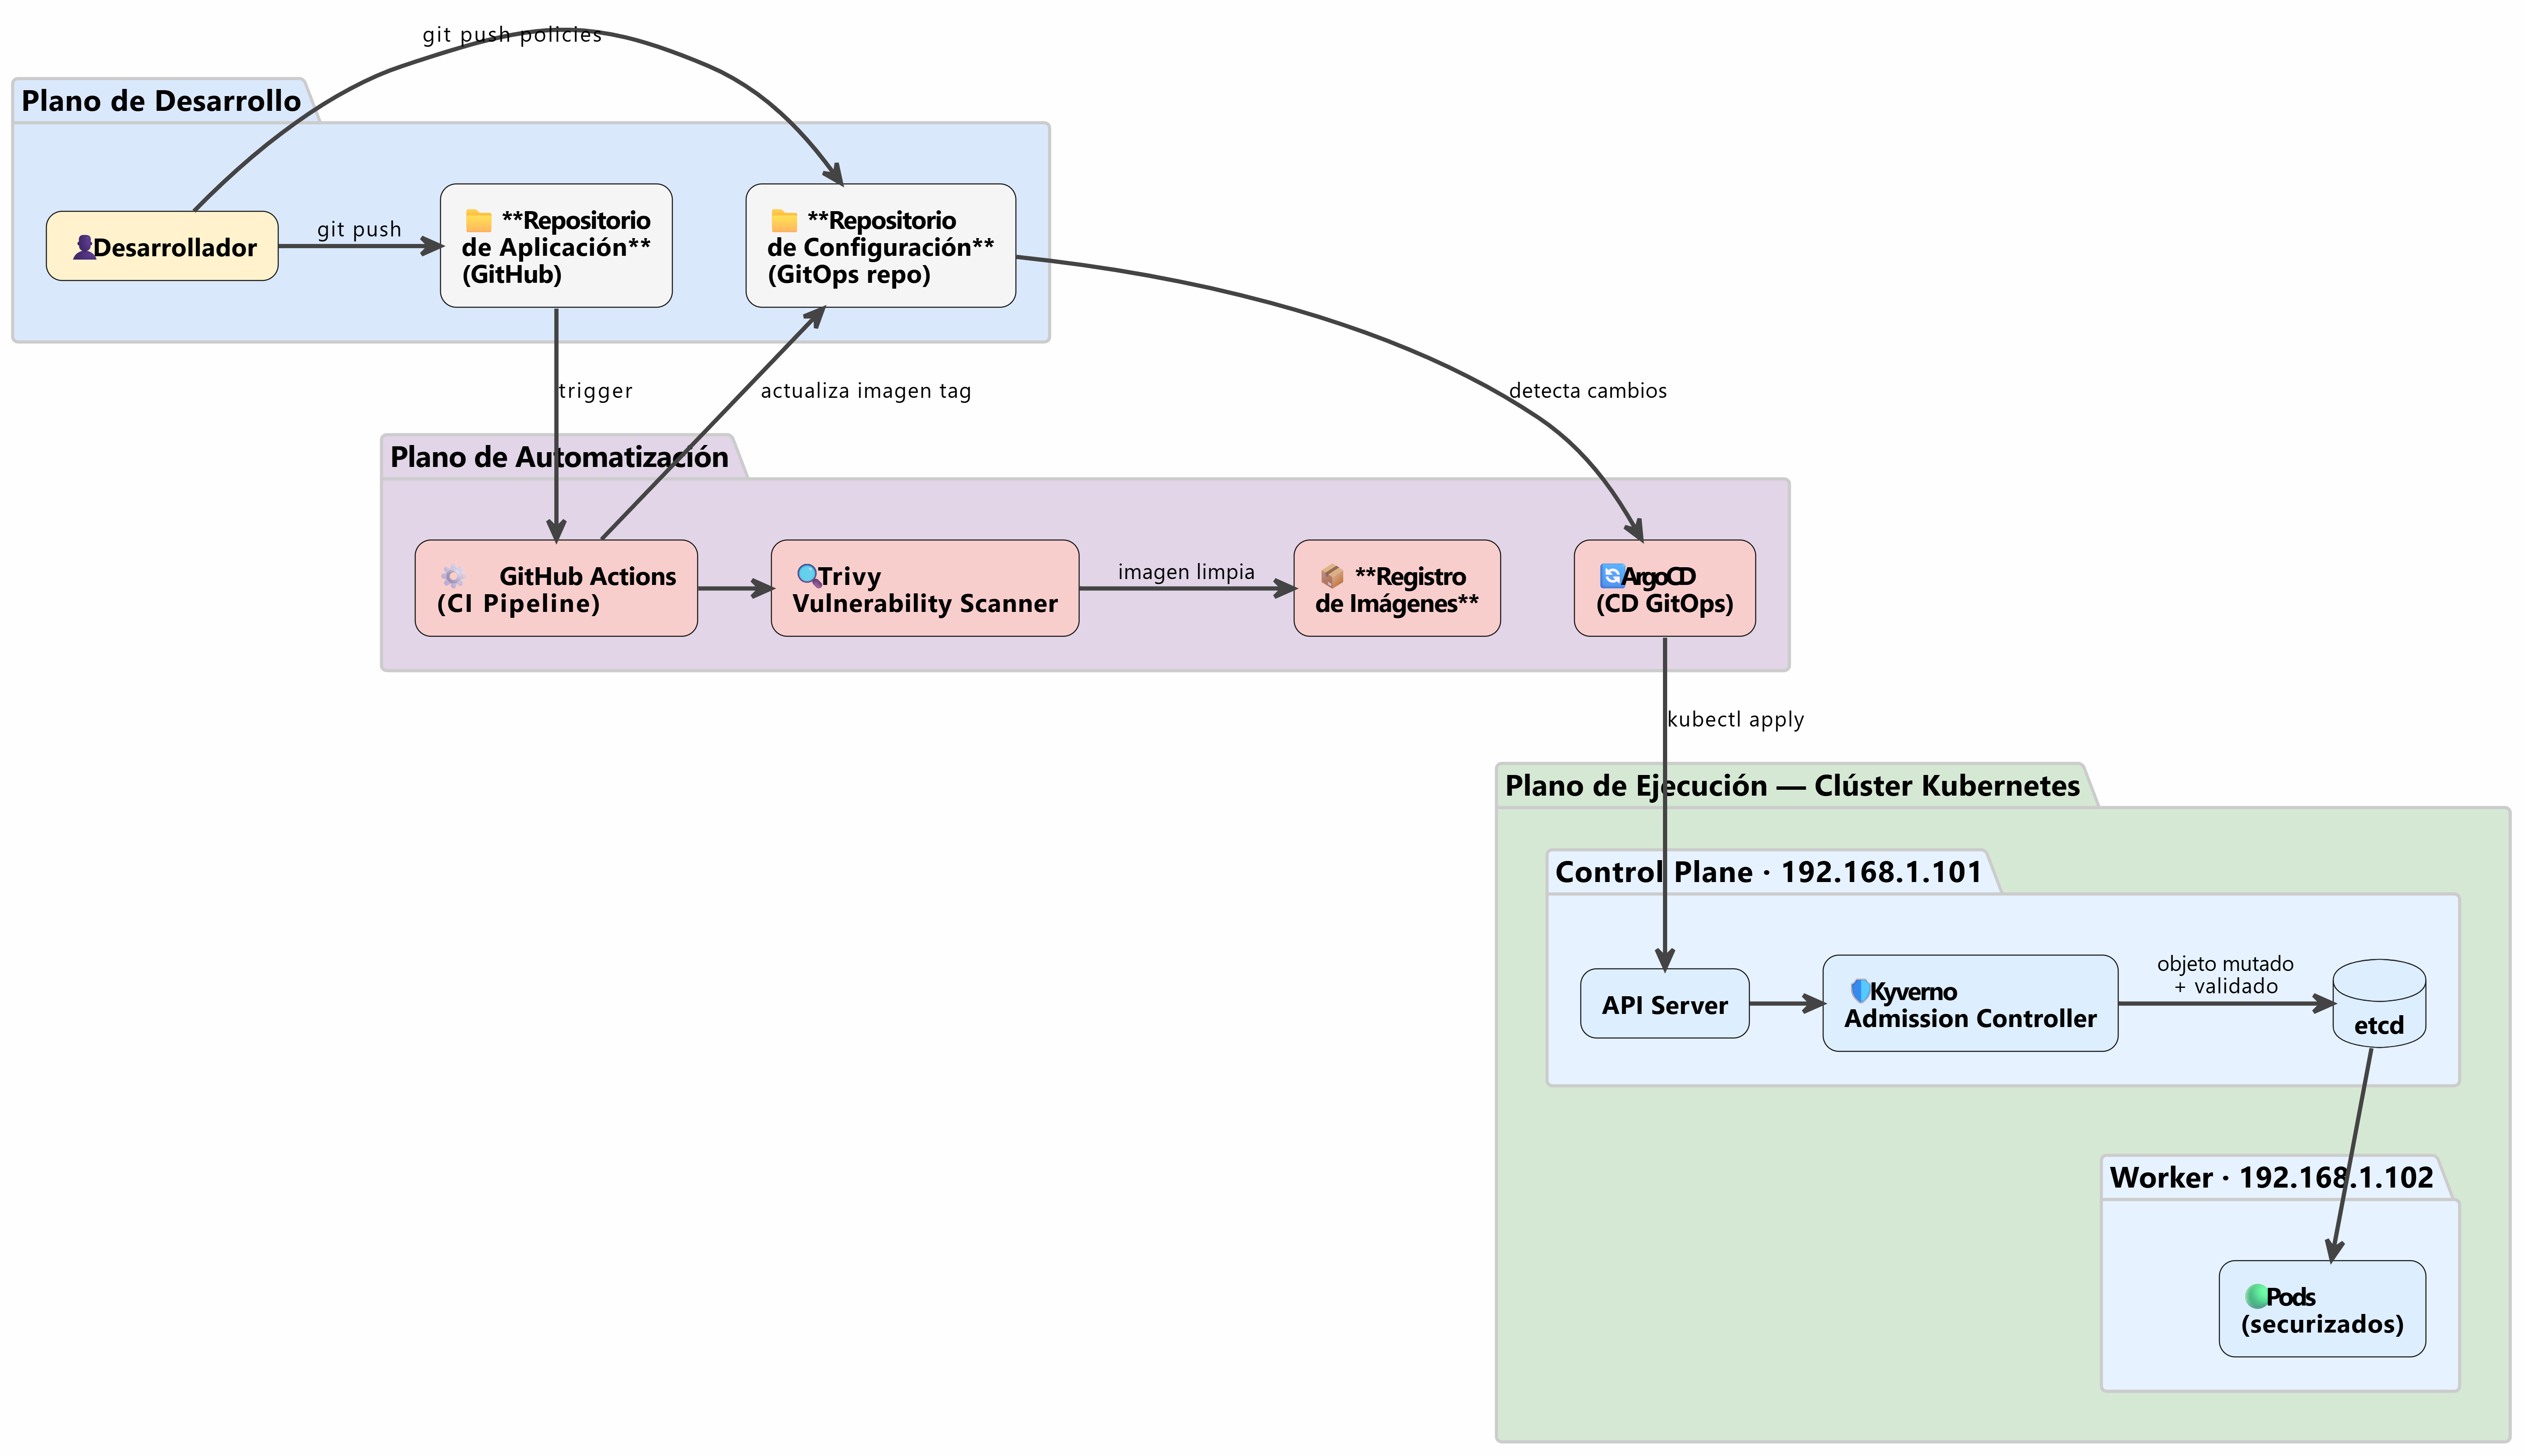
\includegraphics[width=0.95\linewidth]{arquitectura/fig5-1-arquitectura-general.png}
\caption{General architecture of the DevSecOps environment}
\label{fig:arquitectura-general}
\end{figure}

A central architectural aspect is the adoption of the \textbf{two-repository pattern} for the implementation of the GitOps model. The application repository contains the source code of the workloads and business logic, while the configuration repository --- commonly known as the \textit{GitOps repo} --- stores Kubernetes manifests, Kyverno policies and infrastructure configurations. This separation allows the CI pipeline to modify only the configuration repository (updating the image tag after a successful build) without ArgoCD needing access to the application source code, reducing the attack surface and clarifying the responsibilities of each component.

% ─────────────────────────────────────────────
\section{Component description}
% ─────────────────────────────────────────────

\subsection{Kubernetes cluster}

The Kubernetes cluster constitutes the execution platform on which the entire system is based. Following the architecture described in Chapter~4, it consists of two nodes: a control node (\texttt{192.168.1.101}) and a worker node (\texttt{192.168.1.102}), both running Ubuntu Server 24.04 LTS on VirtualBox virtual machines.

The \textbf{API Server} is the central component of the control plane and the only entry point for all cluster operations. All system tools --- ArgoCD, Kyverno, \texttt{kubectl} --- interact exclusively through the API Server, which exposes a RESTful API and applies authentication, authorisation and admission control mechanisms to each received request \cite{kubernetes_docs}. It is precisely in this component where Kyverno's webhooks are registered to intercept admission traffic.

The \textbf{etcd} store persists the complete cluster state as distributed key-value pairs. No resource reaches etcd without having gone through the complete admission process, which guarantees that the persisted state always complies with the defined security policies.

\subsection{Kyverno}

Kyverno is deployed in the dedicated namespace \texttt{kyverno} and operates through four independent controllers, each with well-defined responsibilities \cite{kyverno_docs}:

The \textbf{Admission Controller} is the critical component for this work. It registers in the API Server via two objects of type \texttt{Mutating\-Webhook\-Configuration} and \texttt{Validating\-Webhook\-Configuration}, which instruct the API Server to route admission requests to Kyverno before persisting them. This controller evaluates \textit{mutate} and \textit{validate} policies in real time, with a latency that must remain below the timeout threshold configured in the webhook (by default, 10 seconds).

The \textbf{Background Controller} evaluates policies over resources already existing in the cluster. This is especially relevant for \textit{generate} policies: when the \texttt{generate-networkpolicy-metadata} policy is applied, the Background Controller is responsible for retroactively generating NetworkPolicies in namespaces that already existed before the policy was deployed.

The \textbf{Reports Controller} generates and keeps updated \texttt{PolicyReport} and \texttt{ClusterPolicyReport} resources, which consolidate the results of evaluating all policies over all cluster resources. These reports are fundamental for compliance auditing.

The \textbf{Cleanup Controller} manages the scheduled deletion of resources generated by \textit{generate} policies when the resource that originated them is deleted, maintaining cluster consistency.

\subsection{ArgoCD}

ArgoCD implements the GitOps paradigm by acting as a continuous reconciliation operator between the state declared in the configuration repository and the real state of the cluster \cite{argocd_docs}. Its internal architecture consists of several sub-components: the \textit{Application Controller} is the core that detects state differences (\textit{diff}) and applies reconciliations; the \textit{Repo Server} manages connections to Git repositories and the rendering of manifests; and the \textit{API Server} exposes the user interface and management API.

In the context of this work, ArgoCD manages Kyverno policies like any other Kubernetes resource: the \texttt{ClusterPolicy} objects stored in the configuration repository are automatically synchronised to the cluster. This means that any policy modification --- correction, hardening or new policy --- follows the same versioned approval workflow as any infrastructure change, guaranteeing complete traceability.

ArgoCD's \textit{self-healing} capability directly complements Kyverno's \textit{drift protection} mechanism: if someone manually modifies a policy in the cluster, ArgoCD detects the deviation and reverts it to the state defined in Git; if someone deletes a NetworkPolicy generated by Kyverno, the Background Controller of Kyverno regenerates it. Both layers work in a coordinated manner to guarantee that the system state always remains aligned with what is defined in the repository.

\subsection{GitHub Actions and Trivy}

GitHub Actions acts as the continuous integration engine, running automatically on each \textit{push} to the application repository \cite{github_actions_docs}. The pipeline builds the container image, invokes Trivy to perform a vulnerability analysis \cite{trivy_docs} and, only if the analysis does not detect critical vulnerabilities, publishes the image to the registry and updates the image tag in the configuration repository.

The security of the pipeline itself deserves specific attention. The supervisor's alert about the TeamPCP group attack, which compromised CI/CD pipelines by manipulating third-party GitHub Actions \cite{teampcp2026}, motivates two concrete design decisions detailed in Section~\ref{sec:decisiones}: the anchoring of action versions via SHA hash and the limitation of runner token permissions to the minimum necessary.

\subsection{Sysdig Secure}

Sysdig Secure adds the runtime security dimension to the environment, complementing Kyverno's preventive controls with anomalous behaviour detection during pod execution \cite{sysdig_secure}. As a SaaS service, its integration with the virtual machine-based laboratory environment may present technical limitations, as documented in Chapter~4. Nevertheless, its architectural role is relevant: while Kyverno acts at deployment time, Sysdig Secure acts during execution, covering the attack surface that cannot be statically controlled.

% ─────────────────────────────────────────────
\section{DevSecOps deployment flow}
% ─────────────────────────────────────────────

The complete system flow can be described in two differentiated phases: the continuous integration phase, the responsibility of GitHub Actions, and the continuous deployment phase, the responsibility of ArgoCD and Kyverno. The explicit separation between CI and CD is an intentional architectural decision justified in Section~\ref{sec:decisiones}.

\subsection{Continuous integration phase}

The CI flow begins when a developer performs a \textit{push} to the main branch of the application repository. GitHub Actions detects the event and launches the defined workflow, which executes the following steps sequentially:

First, the container image is built from the repository's Dockerfile. Next, Trivy analyses the resulting image for known vulnerabilities, consulting its CVE database. If the analysis detects critical or high severity vulnerabilities, the pipeline fails at this point and the image is not published, preventing vulnerable code from reaching the execution environment. If the analysis is satisfactory, the image is published to the container registry with a tag that includes the commit hash, guaranteeing traceability between the deployed artefact and the source code that generated it.

The last step of the CI pipeline updates the deployment manifest in the configuration repository, replacing the previous image tag with the new one. This commit in the configuration repository acts as a trigger signal for the CD phase.

Figure~\ref{fig:flujo-cicd} illustrates this complete CI/CD flow.

\begin{figure}[htbp]
\centering
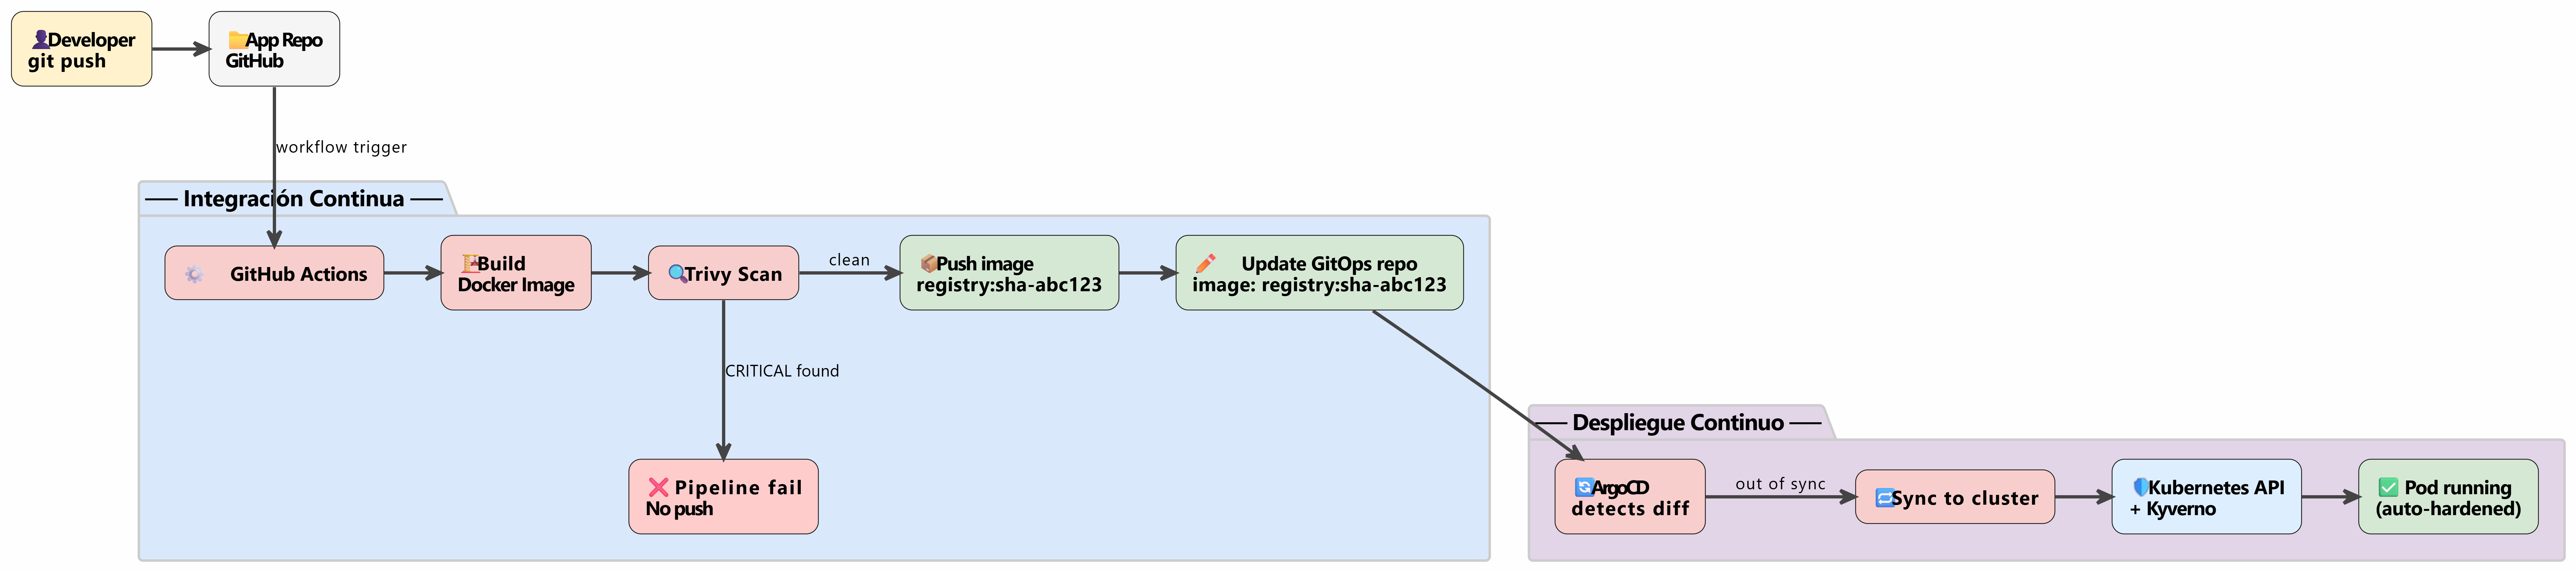
\includegraphics[width=0.95\linewidth]{arquitectura/fig5-2-flujo-cicd.png}
\caption{Continuous integration and deployment flow with security analysis}
\label{fig:flujo-cicd}
\end{figure}

\subsection{Continuous deployment and admission phase}

ArgoCD periodically monitors the configuration repository. Upon detecting the new commit introduced by the CI pipeline, it computes the difference between the updated manifest and the current cluster state and initiates synchronisation, sending the resource update request to the Kubernetes API Server.

At this point, Kyverno intervenes through the Admission Controllers mechanism. The Kubernetes admission process follows a determined sequence \cite{kubernetes_docs} illustrated in Figure~\ref{fig:flujo-admision}:

\begin{figure}[htbp]
\centering
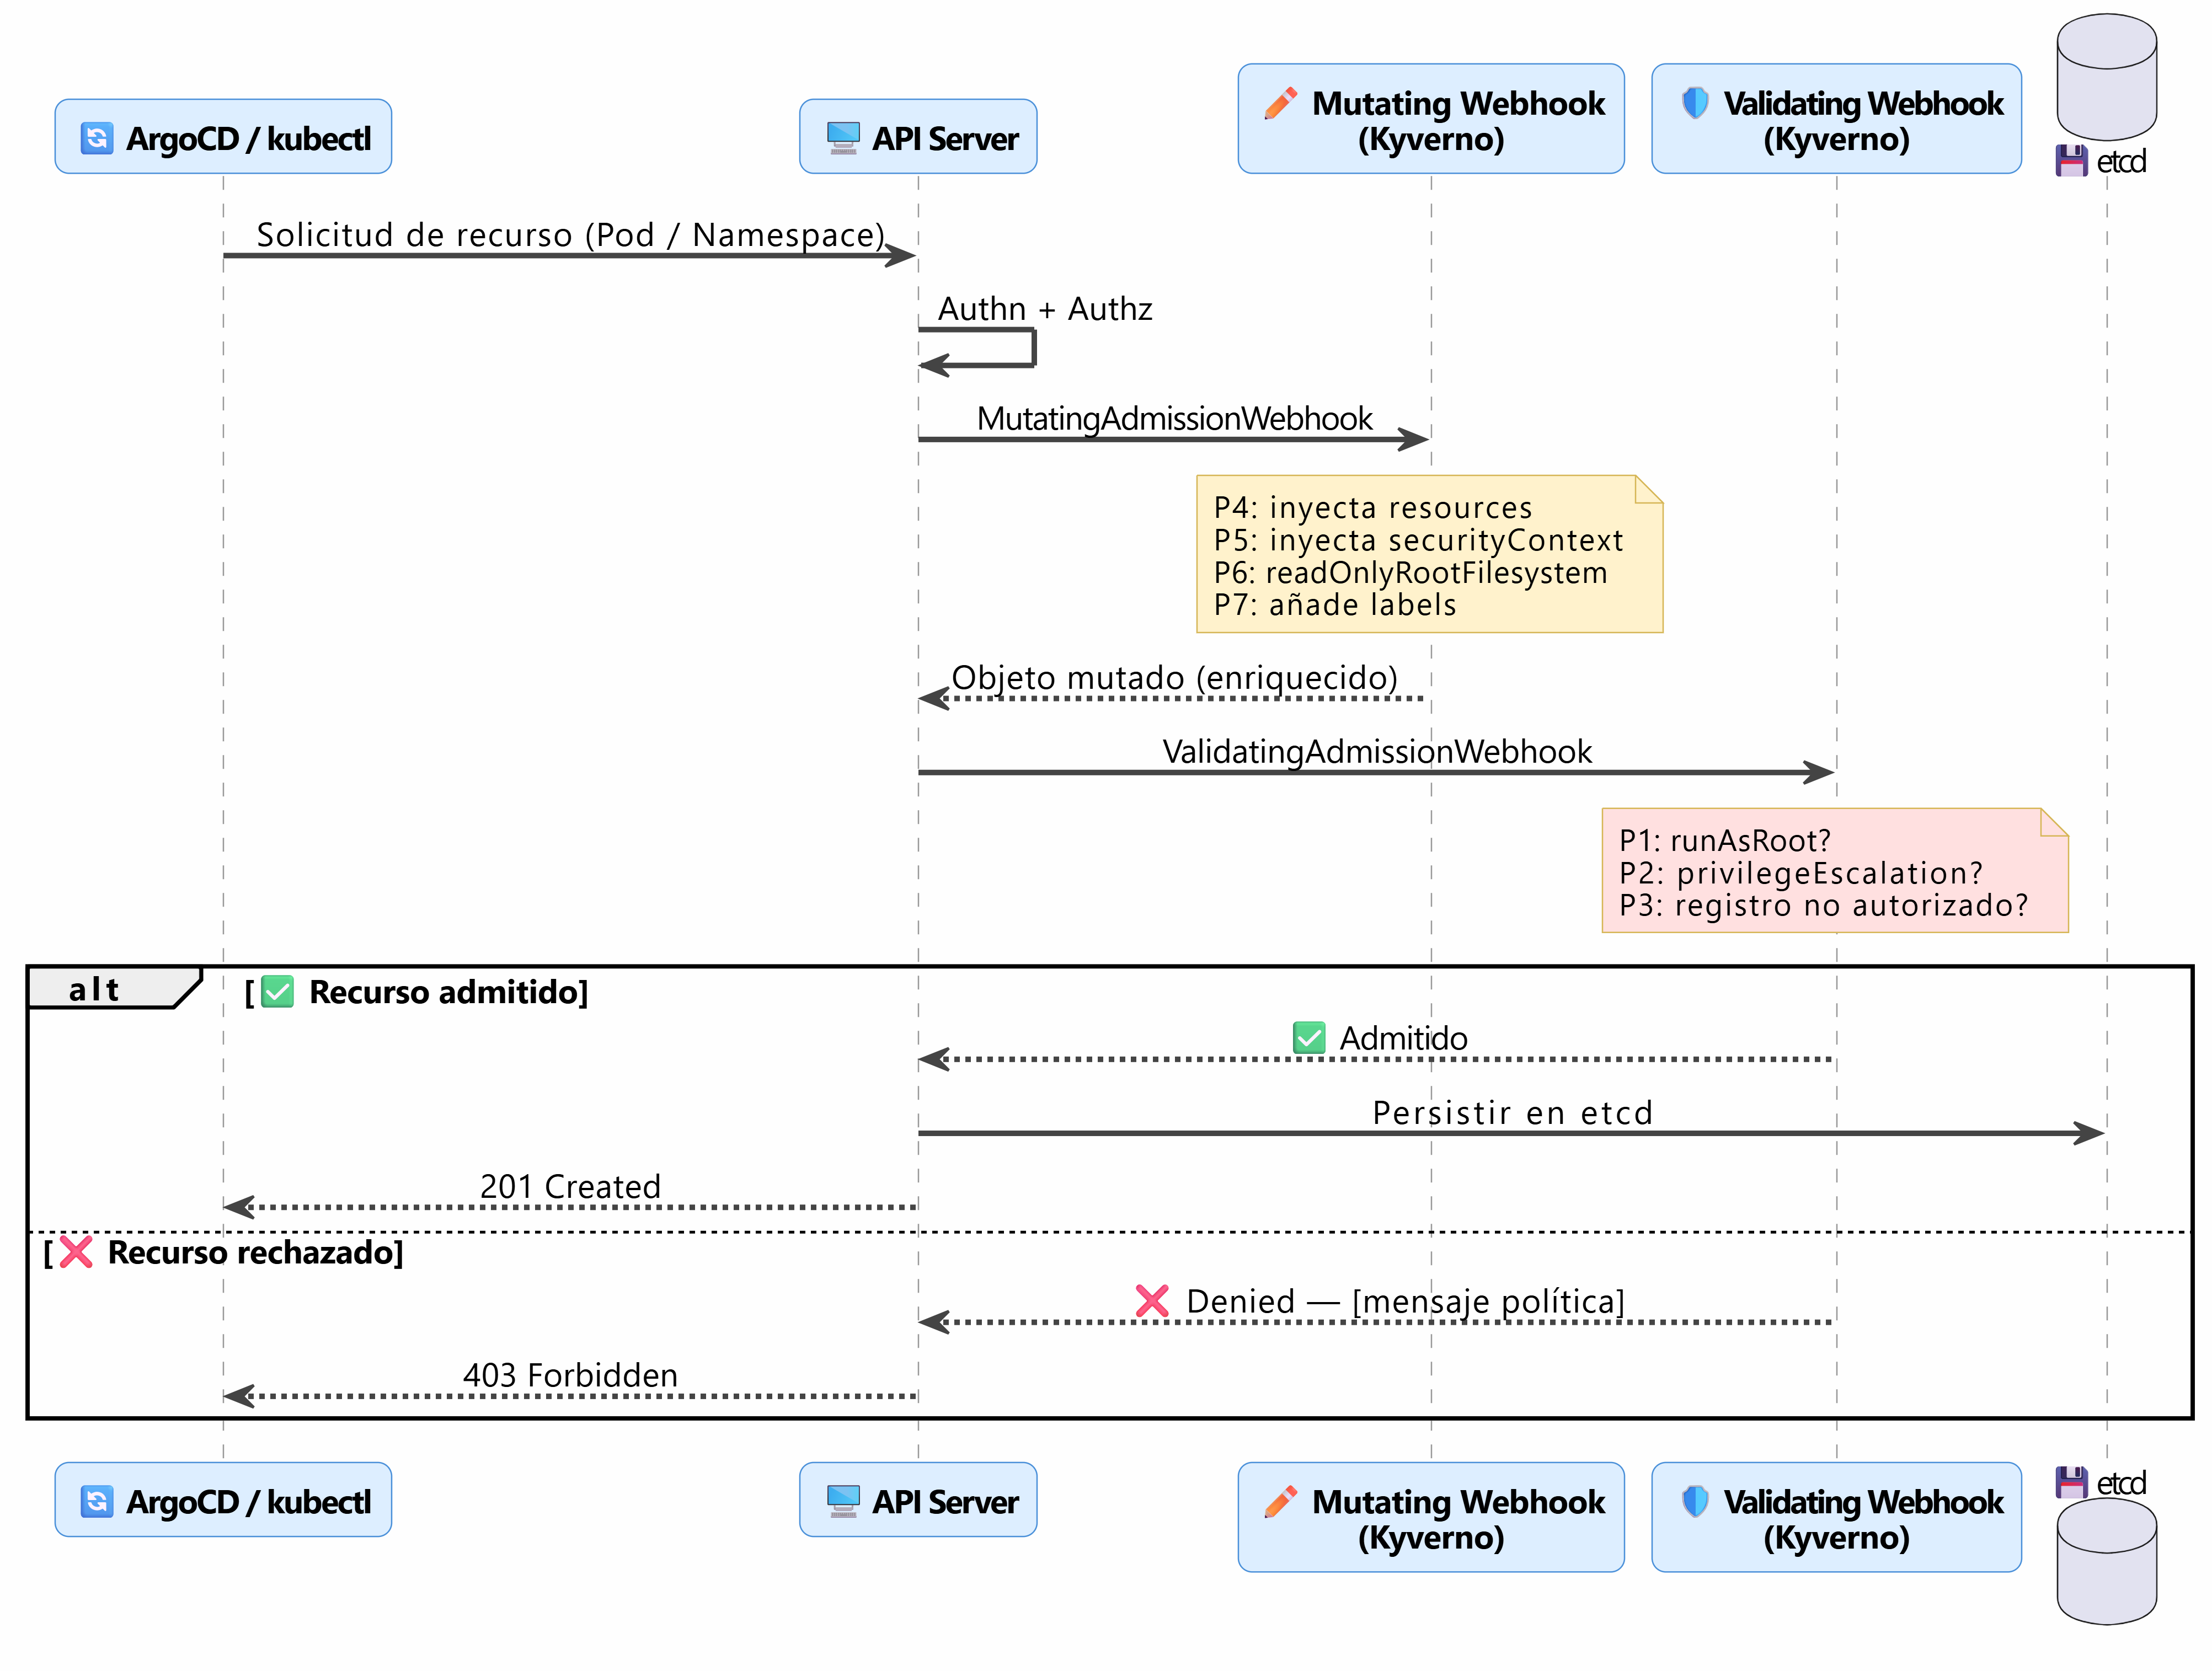
\includegraphics[width=0.90\linewidth]{arquitectura/fig5-3-flujo-admision.png}
\caption{Kyverno admission flow: mutation before validation}
\label{fig:flujo-admision}
\end{figure}

After request authentication and authorisation, the API Server invokes the registered \textit{mutating admission webhooks}. Kyverno receives the object in its original state and sequentially applies all active \textit{mutate} policies: it injects CPU and memory limits and requests (P4), completes the container's \texttt{securityContext} with the missing secure configurations (P5), forces the read-only filesystem (P6) and adds traceability labels (P7). The object returned to the API Server is already the version enriched with all security configurations.

Next, the API Server invokes the \textit{validating admission webhooks}. Kyverno evaluates the \textit{validate} policies over the already mutated object. Since mutation has previously applied the secure configurations, the vast majority of pods pass this validation without rejection. Validation policies act as a final barrier for cases that mutation cannot resolve: the use of images from unauthorised registries (P3), explicit execution as root user when the developer has deliberately specified it (P1) or explicit privilege escalation request (P2). If any validation policy rejects the object, the API Server returns an error with the message defined in the policy and the resource is not persisted in etcd.

If the object passes all admission webhooks, it is persisted in etcd, the Scheduler determines on which node it should run and the kubelet on the worker node proceeds with pod creation.

\section{Cluster network architecture}

The network topology of the laboratory environment is structured in three layers, as shown in Figure~\ref{fig:red-cluster}.

\begin{figure}[htbp]
\centering
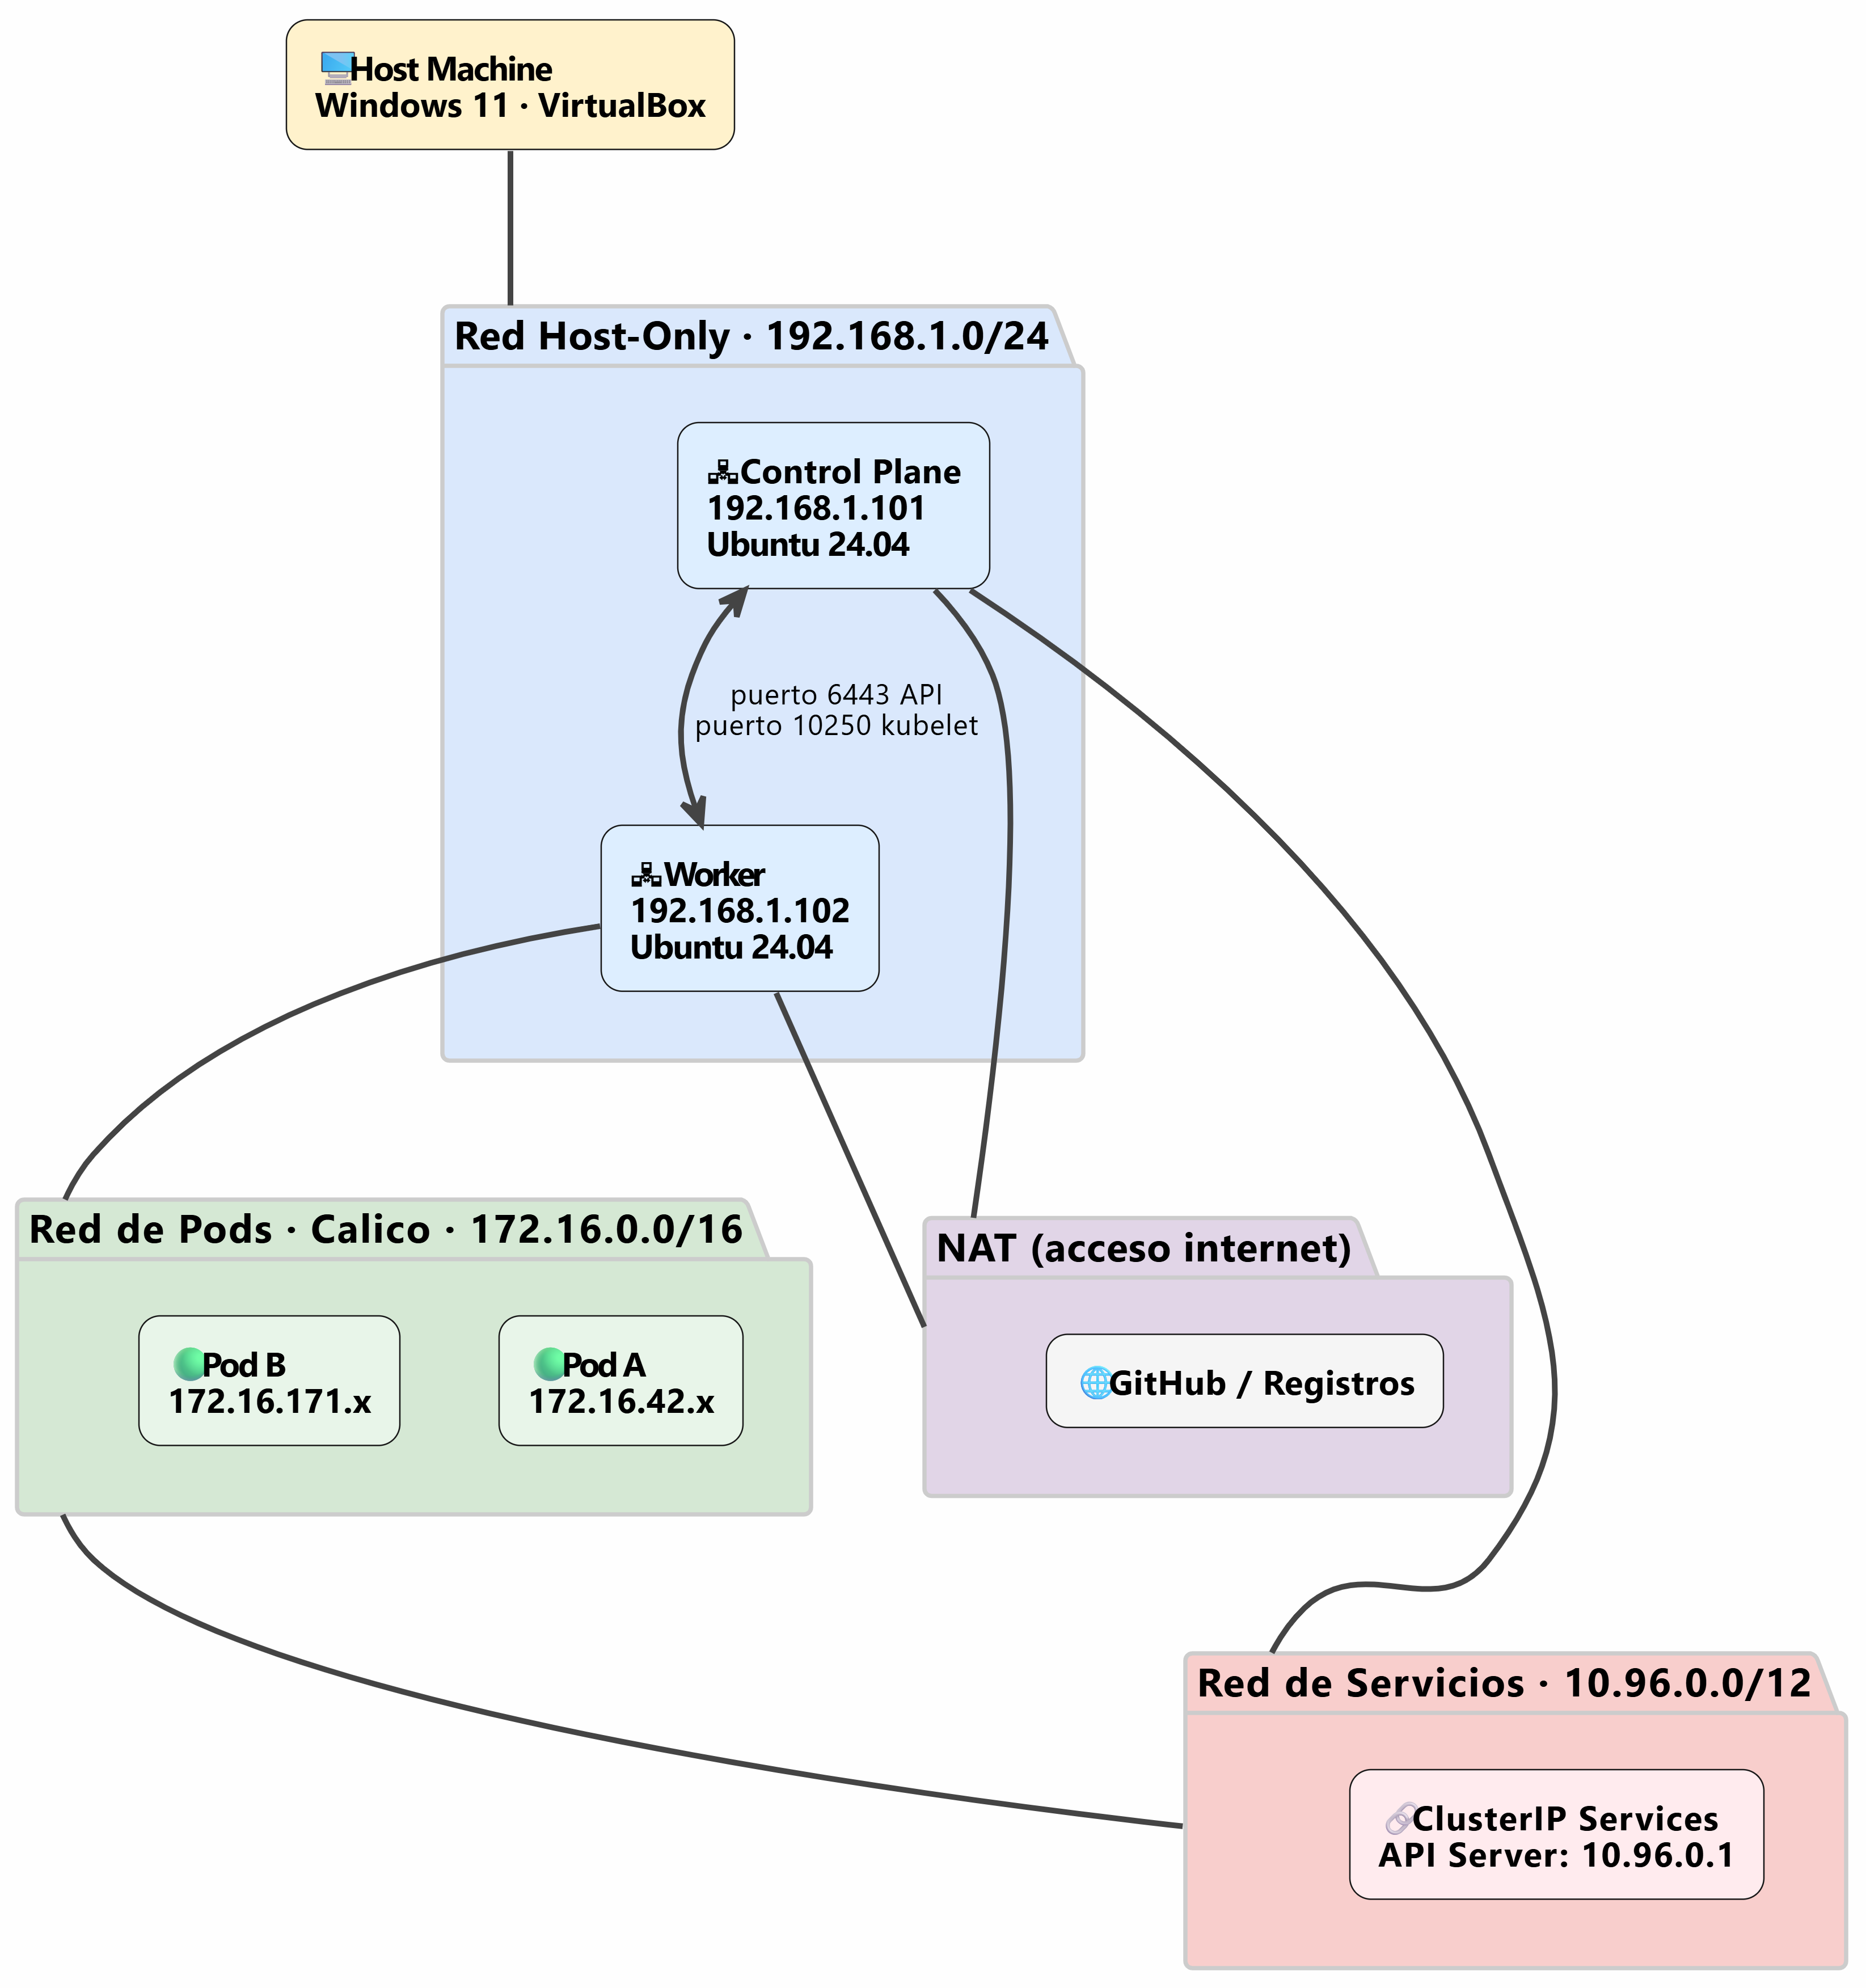
\includegraphics[width=0.85\linewidth]{arquitectura/fig5-4-red-cluster.png}
\caption{Network architecture of the laboratory cluster}
\label{fig:red-cluster}
\end{figure}

The \textbf{management layer} corresponds to VirtualBox's \textit{host-only} network (\texttt{192.168.1.0/24}), through which the host machine and both cluster nodes communicate. The nodes have statically assigned IP addresses: \texttt{192.168.1.101} for the control node and \texttt{192.168.1.102} for the worker node. All internal cluster communication --- between the API Server and kubelets, between the API Server and Kyverno and ArgoCD controllers --- transits through this network. Additionally, each node has a VirtualBox NAT interface that provides internet access, used for downloading container images and communication with external services such as GitHub or image registries.

The \textbf{pod layer} is managed by Calico \cite{calico_docs}, which assigns a private addressing space (\texttt{172.16.0.0/16}) to cluster pods. Calico implements Kubernetes Network Policies through \texttt{iptables} or eBPF rules, depending on the configuration, guaranteeing that the traffic restrictions defined in the policies are applied effectively. This implementation is a requirement for the project's policy P8: the NetworkPolicy generated by Kyverno to block access to the cloud metadata service (\texttt{169.254.169.254/32}) only takes effect if the underlying CNI plugin respects and applies Kubernetes Network Policies, a condition that Calico natively meets.

The \textbf{service layer} uses the addressing space \texttt{10.96.0.0/12}, reserved by kubeadm for \texttt{ClusterIP} type \texttt{Service} objects. The services of system components --- API Server (\texttt{10.96.0.1}), ArgoCD Server, Kyverno --- are accessible within the cluster through this address space, while external access to the API Server is achieved directly through the control node IP via port 6443.

% ─────────────────────────────────────────────
\section{Design decisions}
\label{sec:decisiones}
% ─────────────────────────────────────────────

The architectural decisions adopted in the system design are not arbitrary, but respond to specific technical and security requirements. This section documents the most relevant ones and justifies each of them.

\subsection{Separation between CI and CD}

The separation between continuous integration (GitHub Actions) and continuous deployment (ArgoCD) is a deliberate architectural decision, rather than a single pipeline that builds and deploys in one sequence. This separation offers several advantages. First, it decouples the necessary credentials: the CI pipeline needs access to the image registry and configuration repository, but not to the Kubernetes cluster; ArgoCD has access to the cluster but not to the source code. This segregation reduces the blast radius of a possible compromise of either component. Second, it allows applying security controls at the boundary between the two phases: the image is only published if it passes the Trivy analysis, and ArgoCD only deploys what is in the configuration repository, which acts as an audited control point.

\subsection{ClusterPolicy scope vs. Policy}

Kyverno allows defining policies with cluster scope (\texttt{ClusterPolicy}) or namespace scope (\texttt{Policy}). In this work, exclusively \texttt{ClusterPolicy} objects are used, which guarantees that security policies apply to all cluster namespaces without exceptions. A namespaced policy could inadvertently be omitted when creating a new namespace, creating a coverage gap. The use of \texttt{ClusterPolicy} implements the \textit{secure by default} principle: security is applied everywhere unless explicitly excluded through documented exception rules.

\subsection{Enforce mode vs. Audit mode}

Kyverno can operate in two modes: \texttt{Enforce}, which actively blocks resources that violate policies, and \texttt{Audit}, which allows deployment but records violations in PolicyReports. In this work, validation policies operate in \texttt{Enforce} mode, which guarantees that no non-compliant resource reaches the cluster. Although in a real production environment it is usually recommended to start in \texttt{Audit} mode to avoid disruptions, in the context of this laboratory environment \texttt{Enforce} mode is what effectively demonstrates the blocking mechanism and its real effect on deployments.

\subsection{Mutation before validation as a hardening strategy}

The Kubernetes webhook execution order --- mutation before validation --- is deliberately leveraged as an automatic \textit{hardening} strategy. Mutation policies are not optional complements, but the main security mechanism of the system: instead of rejecting pods with incomplete configurations (which would create friction for developers), Kyverno automatically completes them with the correct security profile. Validation policies act only on configurations that cannot be resolved through mutation, such as the use of unauthorised image registries or the presence of explicitly declared privileges.

This strategy aligns security with usability: the developer can work with minimal manifests and obtain a correctly secured pod without needing to know in detail all Kubernetes security fields. The responsibility for compliance rests on the platform, not on the developer.

\subsection{synchronize: true in generation policies}

Policy P8 uses the \texttt{synchronize: true} field in its \textit{generate} type definition. This configuration instructs Kyverno's Background Controller to monitor generated resources and recreate them automatically if they are deleted or modified in an unauthorised manner. This decision implements the \textit{drift protection} principle at the level of security resources: the NetworkPolicy that blocks access to the IMDS cannot be permanently deleted by an operator (intentionally or accidentally), as Kyverno will regenerate it within seconds. Without this field, generation would be a one-time event and protection could be circumvented.

\subsection{Pipeline supply chain security}

The compromise of the TeamPCP group over CI/CD pipelines \cite{teampcp2026} illustrates that the automation pipeline itself can become an attack vector. In response to this threat, the pipeline design adopts two concrete measures. The first is the anchoring of GitHub Actions versions via their full SHA hash, rather than floating tags such as \texttt{@latest} or \texttt{@v3}, which can be redirected to malicious versions without modifying the reference name. The second is the configuration of the GitHub token with minimum permissions (\textit{least privilege}): the runner only has the permissions strictly necessary for its function, limiting the impact of a possible compromise of the execution environment.

\subsection{Choice of Calico as CNI plugin}

The choice of Calico \cite{calico_docs} over alternatives such as Flannel or Weave responds to a direct functional requirement: policy P8 requires that Kubernetes Network Policies be effectively applied by the CNI plugin. Flannel, for example, does not natively support Network Policies. Calico, on the other hand, is one of the reference CNI plugins in production environments and provides a complete implementation of the Kubernetes Network Policy model, guaranteeing that the traffic blocking rules generated by Kyverno have a real effect on pod network communication.

\chapter{Cluster Implementation and Security Policies}

This chapter documents the practical implementation of the Kubernetes cluster and the policy engine that constitute the security core of the environment designed in Chapter~5. Unlike that chapter, which establishes architectural decisions and their theoretical justification, this chapter focuses on concrete execution: the steps carried out, the deployed policies with their complete manifests, the executed tests and the observed results. The implementation of the DevSecOps pipeline automation components --- ArgoCD for continuous deployment and GitHub Actions for continuous integration --- is addressed in the following chapters.

The chapter is structured into seven sections. The first covers Kubernetes cluster provisioning on the laboratory environment. The second describes Kyverno deployment and the verification of its integration with the API Server. The third, fourth and fifth sections document respectively the implementation of validation, mutation and generation policies, with their manifests, technical justifications and associated tests. The sixth section collects the most relevant operational considerations and empirical findings of the process, including the verification of webhook execution order and the integral \textit{auto-hardening} test. The chapter closes with the seventh section, dedicated to Policy Reports as the native compliance audit mechanism.

% ─────────────────────────────────────────────
\section{Kubernetes cluster provisioning}
% ─────────────────────────────────────────────

The starting point of the project is the provisioning of a functional Kubernetes cluster on the laboratory environment described in Section~4.2. The virtual machines, provided by the supervisor, run Ubuntu Server 24.04~LTS and are pre-configured with the necessary packages (\texttt{kubeadm}, \texttt{kubelet}, \texttt{kubectl}) and with the VirtualBox network layer in NAT plus \textit{host-only adapter} mode.

The control plane is initialised from the \texttt{control} node using the following command:

\begin{lstlisting}
sudo kubeadm init --apiserver-advertise-address=192.168.1.101
\end{lstlisting}

The \texttt{-{}-apiserver-advertise-address} parameter is necessary in environments with multiple network interfaces to indicate to kubeadm on which address the API Server should listen. Without this parameter, kubeadm would select the default interface, which in VirtualBox corresponds to the NAT adapter (\texttt{10.0.2.x}), inaccessible from the worker node. By specifying the \textit{host-only} interface address, it is guaranteed that cluster components --- including Kyverno's webhooks --- are reachable through the laboratory's internal network.

After initialisation, \texttt{kubectl} access is configured for the \texttt{student} user by copying the configuration file generated by kubeadm:

\begin{lstlisting}
mkdir -p $HOME/.kube
sudo cp -i /etc/kubernetes/admin.conf $HOME/.kube/config
sudo chown $(id -u):$(id -g) $HOME/.kube/config
\end{lstlisting}

Next, the worker node (\texttt{192.168.1.102}) joins the cluster via the \texttt{kubeadm join} command generated during initialisation, which includes the bootstrap token and the API Server certificate hash to guarantee connection authenticity.

Once both nodes form part of the cluster, the Calico CNI plugin version 3.28 is installed:

\begin{lstlisting}
kubectl apply -f https://raw.githubusercontent.com/projectcalico/calico/v3.28.0/manifests/calico.yaml
\end{lstlisting}

Calico configures the pod addressing space with the CIDR \texttt{172.16.0.0/16}, the default value for this distribution. Once installation is complete and after system component convergence, the cluster reaches operational state with both nodes in \texttt{Ready} state.

% ─────────────────────────────────────────────
\section{Kyverno deployment and integration}
% ─────────────────────────────────────────────

With the cluster operational, the next step is the installation of Kyverno as the security policy engine. Kyverno is deployed via Helm in the dedicated namespace \texttt{kyverno}:

\begin{lstlisting}
helm repo add kyverno https://kyverno.github.io/kyverno/
helm repo update
helm install kyverno kyverno/kyverno -n kyverno --create-namespace
\end{lstlisting}

After installation, the verification of pod state in the \texttt{kyverno} namespace confirms that the four controllers are active and in \texttt{Running} state, as shown in Figure~\ref{fig:kyverno-pods}.

\begin{figure}[htbp]
\centering
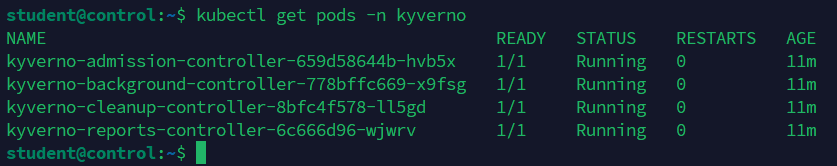
\includegraphics[width=0.85\linewidth]{kyverno/compKyverno.png}
\caption{Kyverno controllers deployed in the cluster}
\label{fig:kyverno-pods}
\end{figure}

The four controllers --- \texttt{admission-controller}, \texttt{background-controller}, \texttt{cleanup-\allowbreak controller} and \texttt{reports-controller} --- operate independently and complementarily, as described in Section~5.2.2. The most relevant controller for the system's real-time behaviour is the \textit{admission controller}, which registers in the API Server immediately after its deployment.

The verification of registered webhooks confirms that Kyverno has correctly established its integration with the API Server. The query of \texttt{Validating\allowbreak{}WebhookConfiguration} objects shows seven configurations registered by Kyverno, as seen in Figure~\ref{fig:kyverno-webhooks}.

\begin{figure}[htbp]
\centering
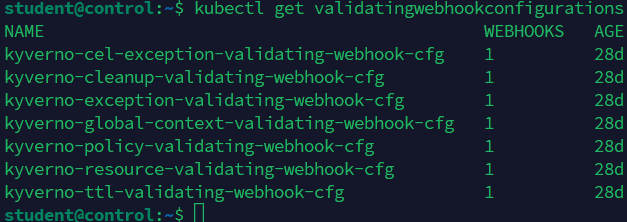
\includegraphics[width=0.85\linewidth]{kyverno/webhooksKyverno.png}
\caption{ValidatingWebhookConfigurations registered by Kyverno in the API Server}
\label{fig:kyverno-webhooks}
\end{figure}

Among the registered configurations, the most relevant for this work is \texttt{kyverno-resource-\allowbreak{}validating-\allowbreak{}webhook-\allowbreak{}cfg}, which intercepts creation and modification requests for arbitrary cluster resources and routes them to Kyverno's \textit{admission controller} for evaluation. The additional configurations cover specific cases such as policy validation itself (\texttt{kyverno-policy-\allowbreak{}validating-\allowbreak{}webhook-\allowbreak{}cfg}), global context (\texttt{kyverno-global-context-\allowbreak{}validating-\allowbreak{}webhook-\allowbreak{}cfg}) and exception and TTL management. Similarly, Kyverno registers the corresponding \texttt{Mutating\allowbreak{}Webhook\allowbreak{}Configuration} objects for processing \textit{mutate} policies.

With Kyverno installed and its webhooks active, the cluster is ready to receive security policies. Figure~\ref{fig:estado-inicial} shows the cluster state at this point, before applying any policy: the \texttt{ClusterPolicy} query returns no resources.

\begin{figure}[htbp]
\centering

\includegraphics[width=0.58\linewidth]{kyverno/estadoInicial.png}
\caption{Initial cluster state: no policies deployed}
\label{fig:estado-inicial}
\end{figure}

% ─────────────────────────────────────────────
\subsection{Kyverno's autogen mechanism}
\label{subsec:autogen}
% ─────────────────────────────────────────────

Before documenting the implemented policies, it is necessary to understand a mechanism that conditions the real scope of all of them: automatic rule generation, known as \textit{autogen}.

\subsubsection*{The problem: Pods are rarely created directly}

The eight policies in this work declare \texttt{match.resources.kinds:\,[Pod]}, which appears to restrict their application to \texttt{Pod} type resources. However, in practice Pods are not created directly: they are generated by higher-level controllers --- \texttt{Deployment}, \texttt{StatefulSet}, \texttt{DaemonSet}, \texttt{Job}, \texttt{CronJob}, \texttt{ReplicaSet} --- through a \texttt{spec.template} field that contains the specification of the Pod to be instantiated.

If Kyverno only evaluated resources of type \texttt{Pod}, a developer --- or an attacker --- could create a \texttt{Deployment} with insecure configuration without the policy intercepting it. The Pods derived from that Deployment would be individually rejected by the \textit{admission webhook} when the controller tried to create them, but the \texttt{Deployment} object would remain persisted in etcd and the controller would enter a loop of recurring errors, generating operational noise and leaving the root resource in an inconsistent state. In permissive failure modes, depending on the webhook's \texttt{failurePolicy} configuration, some resources might even manage to execute.

\subsubsection*{The solution: auto-generated rules}

Kyverno solves this problem transparently for the policy author. When processing a \texttt{ClusterPolicy} that declares \texttt{match.kinds:\,[Pod]}, the engine analyses the defined pattern and automatically generates additional rules --- called \textit{autogen rules} --- that apply the same control over the \texttt{spec.template.spec} of controllers that create Pods. The developer defines the policy once and Kyverno internally replicates it to cover \texttt{Deployment}, \texttt{StatefulSet}, \texttt{DaemonSet}, \texttt{Job}, \texttt{CronJob} and \texttt{ReplicaSet}.

Generation distinguishes two cases depending on nesting depth. For most controllers, the auto-generated rule is called \texttt{autogen-<original-name>} and applies the pattern over \texttt{spec.template.spec}. For \texttt{CronJob}, whose Pod specification is one level deeper (\texttt{spec.jobTemplate.\allowbreak{}template.spec}), Kyverno generates a second additional rule, \texttt{autogen-cronjob-<original-name>}, which adjusts the pattern path accordingly.

The empirical verification of this behaviour is carried out by inspecting the \texttt{ClusterPolicy} object once deployed:

\begin{lstlisting}
kubectl get clusterpolicy disallow-root -o yaml | grep -A 50 "autogen:"
\end{lstlisting}

The output of this command shows the rules \texttt{autogen-require-run-as-non-root}, covering Deployments, StatefulSets, Jobs and CronJobs, and \texttt{autogen-cronjob-require-run-as-non-root}, handling the specific \texttt{CronJob} case. These rules are generated internally by Kyverno and stored in the policy object in etcd; they do not require any manual intervention from the operator.

\subsubsection*{Differentiated behaviour: validate vs. mutate}

The autogen mechanism does not behave identically for all policy types:

\begin{itemize}
  \item For \textbf{validate} policies, autogen is always automatic and unconditional. Kyverno generates additional rules for all controllers that create Pods without the need for any explicit configuration.
  \item For \textbf{mutate} policies using \texttt{patchStrategicMerge} --- such as the four mutation policies in this work (P4, P5, P6, P7) --- autogen is also automatic. Kyverno adapts the patch so that it applies over the controller's \texttt{spec.template.spec} field, guaranteeing that mutations injected on direct Pods are equally replicated on Pods derived from Deployments or StatefulSets.
  \item For \textbf{mutate} policies using \texttt{patchesJson6902}, autogen is not applied by default, since the absolute JSON paths of this mechanism are not automatically generalisable. In these cases, the operator must explicitly configure the autogen behaviour.
\end{itemize}

\subsubsection*{Implication for this work's policies}

The eight implemented policies --- P1 to P8 --- declare \texttt{match.kinds:\,[Pod]}, but thanks to the autogen mechanism they effectively cover Deployments, StatefulSets, Jobs and CronJobs. This means that the real scope of the security system is significantly greater than what can be derived from a direct reading of the manifests.

This behaviour became evident during the initial implementation phases: PolicyViolations generated by the Reports Controller included messages such as \texttt{autogen-require-run-as-non-root} being applied to \texttt{Deployment} and \texttt{ReplicaSet} objects of Kyverno's own components and \texttt{kube-system}, confirming that coverage automatically extended to higher-level resources without having declared those kinds in the policy.

Kyverno allows controlling this behaviour through the annotation \texttt{pod-policies.kyverno.io/\allowbreak{}autogen-controllers} in the policy's \texttt{metadata}, which accepts an explicit list of controllers to cover or the value \texttt{none} to completely disable autogen. In this work the default behaviour is used, which offers the broadest possible coverage without additional configuration.

% ─────────────────────────────────────────────
\section{Validation policies}
% ─────────────────────────────────────────────

Validation policies constitute the reactive layer of the security system: they act by rejecting resources that violate conditions that cannot be resolved through automatic mutation. As justified in Section~5.5.4, mutation policies have precedence and act first; validation policies therefore operate as a final barrier for explicitly insecure configurations that should not be silently corrected, but rejected with a clear message to the requester.

\subsection{Policy P1: \texttt{disallow-root}}

The first validation policy prevents the deployment of pods that do not explicitly specify that their containers must run as a non-root user:

\begin{lstlisting}
apiVersion: kyverno.io/v1
kind: ClusterPolicy
metadata:
  name: disallow-root
spec:
  validationFailureAction: Enforce
  background: true
  rules:
  - name: require-run-as-non-root
    match:
      any:
      - resources:
          kinds:
          - Pod
    validate:
      message: "Containers must not run as root"
      pattern:
        spec:
          securityContext:
            runAsNonRoot: true
\end{lstlisting}

The policy operates through \textit{pattern matching}: Kyverno verifies that the field \texttt{spec.security\allowbreak{}Context.\allowbreak{}runAsNonRoot} exists with the value \texttt{true}. If the field is absent or is \texttt{false}, the webhook returns a validation error with the defined message and the request is rejected.

The technical justification for this control is twofold. On one hand, a process with \texttt{UID~0} inside the container inherits the complete set of Linux capabilities assigned to it, including \texttt{CAP\_SYS\_ADMIN} and \texttt{CAP\_NET\_RAW}, which significantly expand the attack surface. On the other hand, if a container isolation escape occurs --- through a runtime or kernel vulnerability --- a process that was already running as root in the container will obtain root privileges on the host node, potentially compromising the entire cluster.

The validation test applies the following pod, which specifies no \texttt{securityContext}:

\begin{lstlisting}
apiVersion: v1
kind: Pod
metadata:
  name: nginx-insecure
spec:
  containers:
  - name: nginx
    image: nginx
\end{lstlisting}

The result, shown in Figure~\ref{fig:test1}, confirms that Kyverno's webhook rejects the request indicating the exact path of the failing field.

\begin{figure}[htbp]
\centering
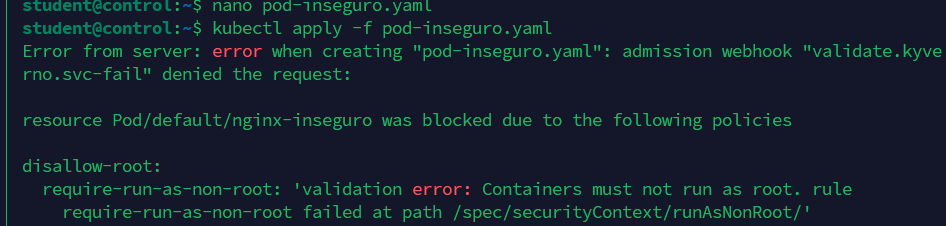
\includegraphics[width=0.95\linewidth]{kyverno/test1.png}
\caption{P1: pod without \texttt{runAsNonRoot} blocked by Kyverno's webhook}
\label{fig:test1}
\end{figure}

\subsection{Policy P2: \texttt{disallow-privilege-escalation}}

The second policy requires all containers to explicitly declare \texttt{allowPrivilege\allowbreak{}Escalation: false} in their container-level \texttt{securityContext}:

\begin{lstlisting}
apiVersion: kyverno.io/v1
kind: ClusterPolicy
metadata:
  name: disallow-privilege-escalation
spec:
  validationFailureAction: Enforce
  rules:
  - name: no-privilege-escalation
    match:
      any:
      - resources:
          kinds:
          - Pod
    validate:
      message: "Privilege escalation is not allowed"
      pattern:
        spec:
          containers:
          - securityContext:
              allowPrivilegeEscalation: false
\end{lstlisting}

This field controls the \texttt{no\_new\_privs} flag of the Linux kernel \cite{linux_no_new_privs}, which prevents any child process from acquiring more privileges than its parent process. Without this flag active, an unprivileged \texttt{UID} process could invoke a binary with the \texttt{SUID} bit active --- such as \texttt{sudo} --- to elevate its privileges to root, circumventing \texttt{runAsNonRoot} controls.

The test applies a pod that explicitly requests privilege escalation. The result, in Figure~\ref{fig:test2}, shows rejection with the path of the offending field.

\begin{figure}[htbp]
\centering
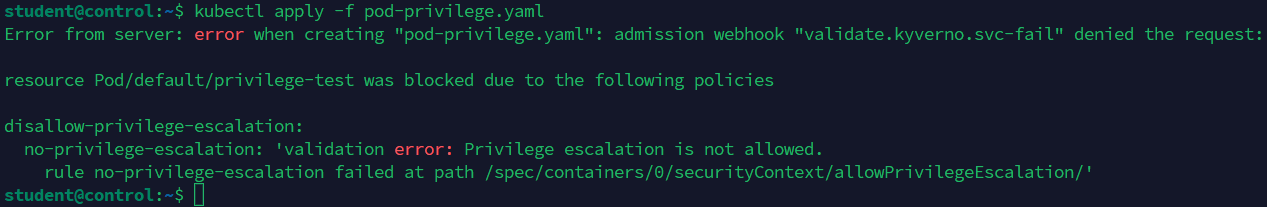
\includegraphics[width=0.95\linewidth]{kyverno/test2.png}
\caption{P2: pod with \texttt{allowPrivilegeEscalation: true} blocked}
\label{fig:test2}
\end{figure}

It is worth noting the interaction between this policy and mutation policy P5. Since \textit{mutating webhooks} are invoked before \textit{validating webhooks}, P5 automatically injects \texttt{allow\-Privilege\-Escalation:\,false} in pods that do not specify this field. Consequently, P2 acts only as a final barrier for cases where the value \texttt{true} has been explicitly declared --- an insecure intention declaration that should not be silently corrected, but rejected.

\subsection{Policy P3: \texttt{restrict-image-registries}}

The third policy restricts image registries to a set of verified sources, implemented via Kyverno's \texttt{foreach} mechanism:

\begin{lstlisting}
apiVersion: kyverno.io/v1
kind: ClusterPolicy
metadata:
  name: restrict-image-registries
spec:
  validationFailureAction: Enforce
  background: true
  rules:
  - name: validate-registries
    match:
      any:
      - resources:
          kinds:
          - Pod
    validate:
      message: >-
        Only images from authorised registries are allowed:
        docker.io, ghcr.io, registry.k8s.io, quay.io.
        The image {{ element.image }} is not permitted.
      foreach:
      - list: "request.object.spec.containers"
        deny:
          conditions:
            all:
            - key: "{{ element.image }}"
              operator: AnyNotIn
              value:
              - "docker.io/*"
              - "ghcr.io/*"
              - "registry.k8s.io/*"
              - "quay.io/*"
              - "nginx*"
              - "alpine*"
              - "busybox*"
              - "nginxinc/*"
\end{lstlisting}

The policy iterates over all pod containers and denies the request if any image does not belong to the authorised patterns. Patterns without registry prefix (\texttt{nginx*}, \texttt{alpine*}, \texttt{busybox*}) are necessary because Kubernetes implicitly resolves unprefixed references to Docker Hub. The inclusion of \texttt{ghcr.io/*} is an operational requirement, given that Kyverno and other cluster component images are distributed through that registry.

This policy constitutes a first line of defence against supply chain attacks of the type documented by the TeamPCP group \cite{teampcp2026}: an attacker who hosts a malicious image on an arbitrary registry will not be able to run it in the cluster without modifying this policy. In mature production environments, the control would be complemented with digital signature verification using Cosign or Notary, considered future work in Section~4.7.

During implementation, a relevant engine behaviour was observed: the variable \texttt{\{\{ element.image \}\}} referenced in the top-level \texttt{message} field does not expand at rejection time, since that variable only has scope within the \texttt{foreach} block. Kyverno accepts the policy as valid and the \texttt{READY} field shows \texttt{True}, but at rejection time the error message only shows the static part, omitting the specific image name. This behaviour illustrates Kyverno's variable scoping model and must be taken into account when designing informative error messages in policies with \texttt{foreach}.

The validation test applies a pod with an image from an unauthorised registry. The result, in Figure~\ref{fig:test3}, reveals a defence-in-depth behaviour: the pod is simultaneously blocked by two independent policies.

\begin{figure}[htbp]
\centering
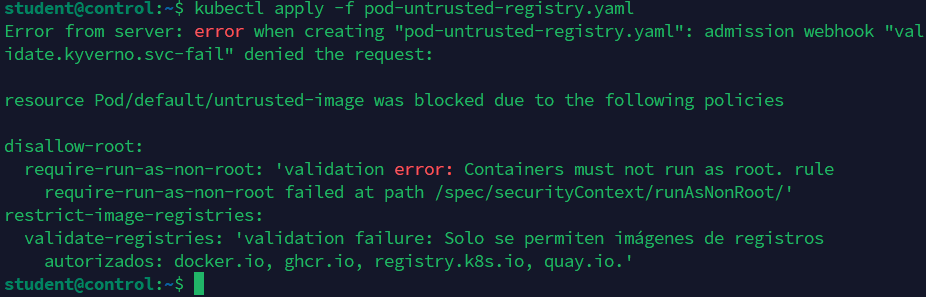
\includegraphics[width=0.95\linewidth]{kyverno/test3.png}
\caption{P3: simultaneous blocking by \texttt{disallow-root} and \texttt{restrict-image-registries}}
\label{fig:test3}
\end{figure}

This result demonstrates that the policy system acts cumulatively: the same resource can violate multiple policies simultaneously, and the error message returned enumerates all detected violations. The image \texttt{evilregistry.io/backdoor:latest} is blocked both for not specifying \texttt{runAsNonRoot} (P1) and for coming from an unauthorised registry (P3), two independent risk vectors detected in a single response.

% ─────────────────────────────────────────────
\section{Mutation policies}
% ─────────────────────────────────────────────

Mutation policies constitute the main security mechanism of the system, aligning with the central hypothesis of the work: that the automatic correction of insecure configurations at admission time offers greater resilience and better development experience than mere rejection. Instead of blocking pods with incomplete configurations, Kyverno automatically enriches them with the correct security profile, making \textit{hardening} transparent to the developer.

The \texttt{patchStrategicMerge} mechanism, used by the four policies in this block, performs an intelligent merge of the original object with the defined patch: it adds absent fields and respects values already explicitly declared by the developer, guaranteeing that mutations are additive and non-destructive.

\subsection{Policy P4: \texttt{add-default-resources}}

The fourth policy automatically injects CPU and memory \texttt{requests} and \texttt{limits} in all containers that do not declare them:

\begin{lstlisting}
apiVersion: kyverno.io/v1
kind: ClusterPolicy
metadata:
  name: add-default-resources
spec:
  rules:
  - name: add-resources
    match:
      any:
      - resources:
          kinds:
          - Pod
    mutate:
      patchStrategicMerge:
        spec:
          containers:
          - (name): "*"
            resources:
              requests:
                cpu: "100m"
                memory: "128Mi"
              limits:
                cpu: "500m"
                memory: "256Mi"
\end{lstlisting}

The simultaneous injection of \texttt{requests} and \texttt{limits} with the same values --- rather than only \texttt{limits} --- responds to a technically justified decision. Kubernetes classifies pods into three Quality of Service classes (\textit{QoS}) \cite{kubernetes_qos}: \texttt{Guaranteed} (when \texttt{requests\,==\,limits} for all containers), \texttt{Burstable} and \texttt{BestEffort}. A pod with \texttt{Guaranteed} QoS is the last candidate for eviction when the node experiences resource pressure. Additionally, without \texttt{requests} defined, the Scheduler lacks information for \textit{bin-packing} decisions and may schedule pods on nodes without sufficient capacity, resulting in OOM failures at runtime.

The test deploys a pod without any \texttt{resources} field defined. As shown in Figure~\ref{fig:test4}, Kyverno automatically injects \texttt{requests} and \texttt{limits} values, visible in the \texttt{kubectl get pod -o yaml} output.

\begin{figure}[htbp]
\centering
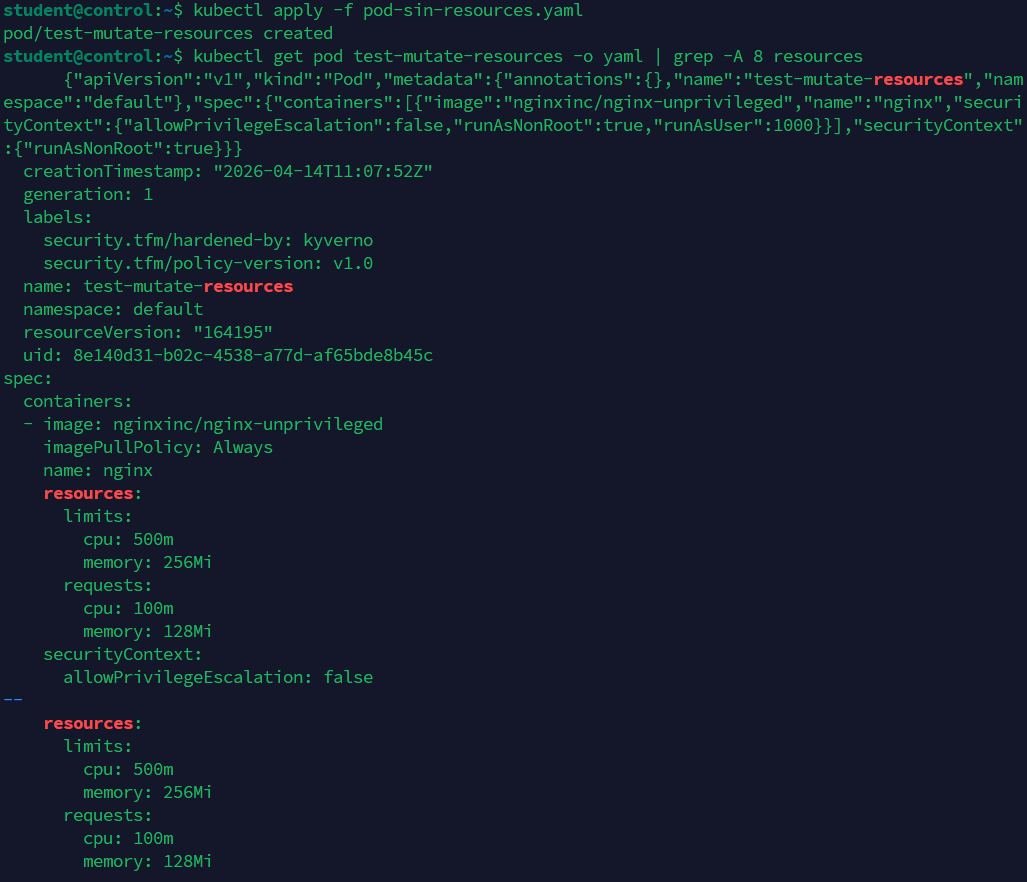
\includegraphics[width=0.95\linewidth]{kyverno/test4.png}
\caption{P4: automatic injection of \texttt{resources.requests} and \texttt{resources.limits}}
\label{fig:test4}
\end{figure}

It is especially significant that the output also shows the labels \texttt{security.tfm/\allowbreak{}hardened-by:\,kyverno} and \texttt{security.tfm/\allowbreak{}policy-version:\,v1.0}, evidence that P7 has also acted on the same resource in the same admission cycle. This confirms that multiple mutation policies are applied in a coordinated manner to each object in a single admission pass.

\subsection{Policy P5: \texttt{add-default-securitycontext}}

The fifth policy injects a secure \texttt{securityContext} in all containers that do not specify one at the container level:

\begin{lstlisting}
apiVersion: kyverno.io/v1
kind: ClusterPolicy
metadata:
  name: add-default-securitycontext
spec:
  rules:
  - name: add-container-security-context
    match:
      any:
      - resources:
          kinds:
          - Pod
    mutate:
      patchStrategicMerge:
        spec:
          containers:
          - (name): "*"
            securityContext:
              allowPrivilegeEscalation: false
              capabilities:
                drop:
                - ALL
\end{lstlisting}

This policy implements two critical \textit{hardening} controls automatically. The first, \texttt{allow\-Privilege\-Escalation:\,false}, activates the kernel's \texttt{no\_new\_privs} flag, preventing privilege escalation through SUID binaries. Here the policy acts \textit{proactively} --- injecting the secure configuration before reaching validation --- in contrast to P2, which acts \textit{reactively} by rejecting the explicit declaration of the insecure value.

The second control, \texttt{capabilities.drop:\,ALL}, removes the complete set of Linux capabilities inherited by default. Without additional configuration, a container inherits capabilities such as \texttt{NET\_RAW} (raw packet construction), \texttt{MKNOD} (block device creation) or \texttt{CHOWN} (file ownership change), which unnecessarily expand the attack surface. By dropping them all by default, developers are forced to explicitly declare the capabilities their applications actually need.

This policy is the most representative example of the \textit{auto-hardening} concept: the developer can deploy a pod with minimal configuration without deep knowledge of Kubernetes security fields, and the platform guarantees a solid security profile in a completely transparent manner.

The test deploys a pod with \texttt{securityContext} defined only at the pod level. Figure~\ref{fig:test5} shows the result: the container-level \texttt{securityContext} contains \texttt{allow\-Privilege\-Escalation:\,false}, \texttt{capabilities.drop:\,[ALL]} and \texttt{readOnly\-Root\-Filesystem:\,true} --- the latter injected by P6 in the same admission cycle.

\begin{figure}[htbp]
\centering
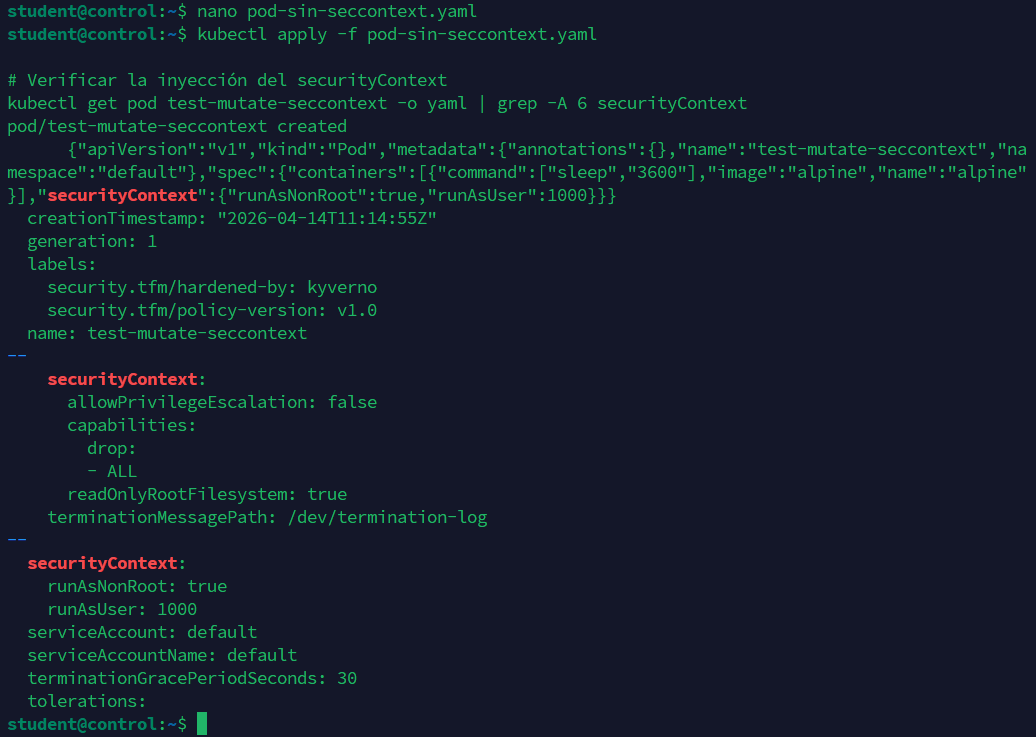
\includegraphics[width=0.95\linewidth]{kyverno/test5.png}
\caption{P5: automatic injection of \texttt{allowPrivilegeEscalation} and \texttt{capabilities.drop}}
\label{fig:test5}
\end{figure}

\subsection{Policy P6: \texttt{add-readonly-rootfs}}

The sixth policy forces the root filesystem of all containers to read-only mode:

\begin{lstlisting}
apiVersion: kyverno.io/v1
kind: ClusterPolicy
metadata:
  name: add-readonly-rootfs
spec:
  rules:
  - name: add-readonly-filesystem
    match:
      any:
      - resources:
          kinds:
          - Pod
    mutate:
      patchStrategicMerge:
        spec:
          containers:
          - (name): "*"
            securityContext:
              readOnlyRootFilesystem: true
\end{lstlisting}

Most post-exploitation techniques after compromising a container --- downloading reverse shells, installing cryptominers, executing reconnaissance tools --- require writing files to the container filesystem. A read-only root filesystem makes these attempts fail immediately, containing the blast radius of the intrusion.

The test verifies this effect in two steps, shown in Figure~\ref{fig:test6}. First, the \texttt{kubectl get pod -o yaml} output confirms that the \texttt{readOnly\-Root\-Filesystem:\,true} field has been injected. Second, a command is executed inside the container that attempts to create a file in the root directory:

\begin{lstlisting}
kubectl exec test-mutate-seccontext -- touch /test-file
touch: /test-file: Read-only file system
command terminated with exit code 1
\end{lstlisting}

\begin{figure}[htbp]
\centering
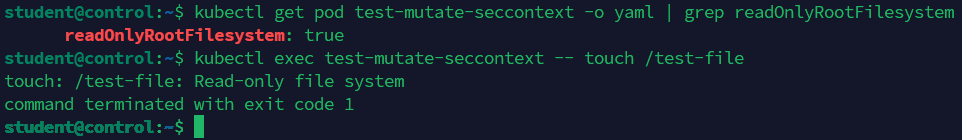
\includegraphics[width=0.90\linewidth]{kyverno/test6.png}
\caption{P6: verification of read-only filesystem at runtime}
\label{fig:test6}
\end{figure}

This result is especially valuable: it demonstrates that the mutation applied by Kyverno at admission time has a real and verifiable effect on container behaviour at runtime, not just on the manifest stored in etcd.

A known operational limitation is that certain applications require writing to directories such as \texttt{/tmp} or \texttt{/var/cache}. The correct solution --- applied in the integral test of Section~6.6.2 --- consists of mounting an \texttt{emptyDir} volume at the specific paths that require write access. This practice does not weaken the policy, but forces developers to be explicit about their write requirements, which is itself a good container design practice.

\subsection{Policy P7: \texttt{add-default-labels}}

The seventh policy injects traceability labels in all pods processed by the system:

\begin{lstlisting}
apiVersion: kyverno.io/v1
kind: ClusterPolicy
metadata:
  name: add-default-labels
spec:
  rules:
  - name: add-security-labels
    match:
      any:
      - resources:
          kinds:
          - Pod
    mutate:
      patchStrategicMerge:
        metadata:
          labels:
            security.tfm/hardened-by: kyverno
            security.tfm/policy-version: "v1.0"
\end{lstlisting}

Although less obvious than direct security policies, this policy implements an observability capability relevant in production environments. The injected labels allow identifying at any time which pods have been processed by the system and with which policy version, facilitating coverage auditing. The \texttt{security.tfm/\allowbreak{}policy-version} field acts as a marker that allows correlating the applied security profile with the policy version in force at the time of deployment.

Verification via \texttt{kubectl get pods --show-labels}, shown in Figure~\ref{fig:test7}, confirms that the labels are present in all active pods in the \texttt{default} namespace.

\begin{figure}[htbp]
\centering
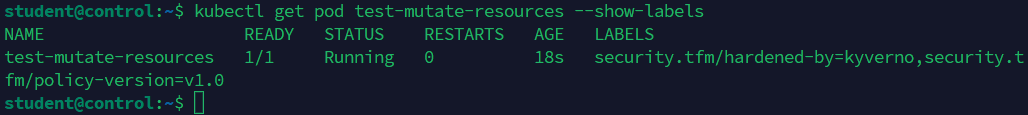
\includegraphics[width=0.90\linewidth]{kyverno/test7.png}
\caption{P7: traceability labels automatically injected in pods}
\label{fig:test7}
\end{figure}

% ─────────────────────────────────────────────
\section{Generation policy}
% ─────────────────────────────────────────────

\subsection{Policy P8: \texttt{generate-networkpolicy-metadata}}

The eighth policy demonstrates the third type of action available in Kyverno --- \textit{generate} --- with no functional equivalent in OPA Gatekeeper. Unlike previous policies, which act on resources in the process of creation, this one reacts to the creation of a \texttt{Namespace} and automatically generates a derived resource: a NetworkPolicy that blocks access to the cloud instance metadata service (IMDS):

\begin{lstlisting}
apiVersion: kyverno.io/v1
kind: ClusterPolicy
metadata:
  name: generate-networkpolicy-metadata
spec:
  rules:
  - name: block-metadata-service
    match:
      any:
      - resources:
          kinds:
          - Namespace
    generate:
      apiVersion: networking.k8s.io/v1
      kind: NetworkPolicy
      name: block-cloud-metadata
      namespace: "{{request.object.metadata.name}}"
      synchronize: true
      data:
        spec:
          podSelector: {}
          policyTypes:
          - Egress
          egress:
          - to:
            - ipBlock:
                cidr: 0.0.0.0/0
                except:
                - 169.254.169.254/32
\end{lstlisting}

The generated NetworkPolicy allows all outgoing traffic (\texttt{cidr:\,0.0.0.0/0}) except towards the address \texttt{169.254.169.254/32}. This IP corresponds to the IMDS present in the main cloud providers (AWS, GCP, Azure), accessible from any instance without prior authentication. An attacker who compromises a pod can make a request to that endpoint to obtain temporary IAM credentials, service tokens and underlying instance network configuration, enabling escalation from the pod to the cloud account. This vector was documentedly used in the Capital One incident in 2019, where SSRF was exploited to access the IMDS and exfiltrate sensitive data \cite{capitalone2019}.

The \texttt{synchronize:\,true} field activates the Background Controller's \textit{drift protection} mechanism: if the generated NetworkPolicy is modified or deleted, Kyverno automatically restores it.

The first test, shown in Figure~\ref{fig:test8}, demonstrates automatic generation: namespace \texttt{test-networkpolicy} is created and just 9~seconds later the NetworkPolicy \texttt{block-cloud-metadata} exists in that namespace without having been manually applied. The detailed description of the generated resource confirms that Kyverno has added the corresponding traceability labels and that the egress rule exclusively blocks IP \texttt{169.254.169.254/32}.

\begin{figure}[htbp]
\centering
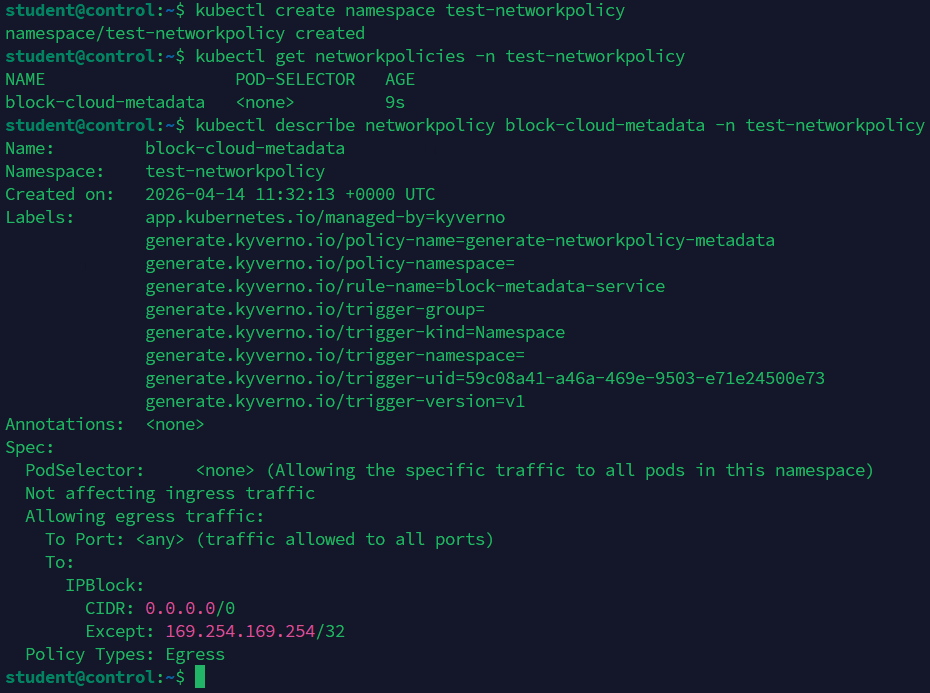
\includegraphics[width=0.95\linewidth]{kyverno/test8.png}
\caption{P8: NetworkPolicy automatically generated upon namespace creation}
\label{fig:test8}
\end{figure}

The second test, shown in Figure~\ref{fig:test9}, demonstrates the \textit{drift protection} mechanism: the NetworkPolicy is manually deleted via \texttt{kubectl delete} and, 57~seconds later, it has been automatically regenerated by the Background Controller, without any human intervention.

\begin{figure}[htbp]
\centering
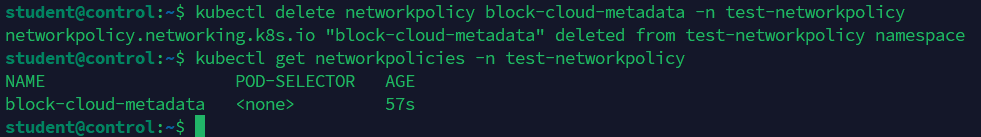
\includegraphics[width=0.90\linewidth]{kyverno/test9.png}
\caption{P8: \textit{drift protection} --- NetworkPolicy regenerated 57~s after manual deletion}
\label{fig:test9}
\end{figure}

This behaviour illustrates a fundamental difference compared to OPA Gatekeeper, which lacks native support for resource generation and cannot implement this pattern of continuous protection.

% ─────────────────────────────────────────────
\section{Operational considerations and lessons learned}
% ─────────────────────────────────────────────

This section collects the most relevant operational findings that emerged during implementation and that do not fit in the individual documentation of each policy. Some of them are directly related to the autogen mechanism described in Section~\ref{subsec:autogen}: the automatic extension of policies to Deployments and ReplicaSets generated friction with ArgoCD during the GitOps pipeline integration phases, as the policies evaluated resources managed by the ArgoCD controller before they were fully compliant. This behaviour is documented in detail in Chapter~7, in the context of the complete pipeline integration.

\subsection{Exclusion of infrastructure namespaces}

During the initial implementation phases, validation policies generated violations on the cluster's own components. In particular, policy P1 (\texttt{disallow-root}) marked certain pods in the \texttt{kube-system} namespace as non-compliant, as they run as root due to functional requirements. In parallel, the first version of P3 (\texttt{restrict-image-\allowbreak{}registries}) did not include the \texttt{ghcr.io/*} pattern, which generated PolicyViolations on Kyverno's own controllers, whose images are distributed via \texttt{ghcr.io/kyverno/}.

The applied solution was twofold: \texttt{ghcr.io/*} was added to the list of authorised registries in P3, correcting the problem structurally; and the policies were revised to exclude infrastructure namespaces in cases where their application is not pertinent. This is a standard practice in Kyverno production deployments, where security policies must be designed with awareness of the system components that execute them. Figure~\ref{fig:rules-aplicadas} shows the final cluster state with all eight policies in \texttt{Ready} state.

\begin{figure}[H]
\centering
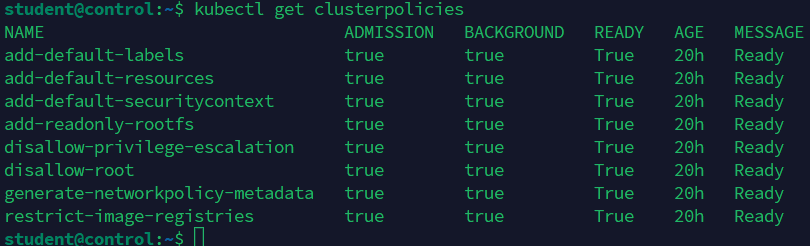
\includegraphics[width=0.95\linewidth]{kyverno/rulesAplicadas.png}
\caption{All eight ClusterPolicies in \texttt{Ready} state after complete deployment}
\label{fig:rules-aplicadas}
\end{figure}

\subsection{Integral auto-hardening test}

The most representative test of the work consists of deploying a pod with deliberately minimal configuration and verifying that the complete set of mutation policies transforms it into a pod with a complete security profile. The initial manifest, shown in Figure~\ref{fig:pod-seguro-yaml}, contains only the fields strictly necessary for operation: image, execution user and an \texttt{emptyDir} volume mounted at \texttt{/tmp} to satisfy policy P6's read-only filesystem requirement.

\begin{figure}[H]
\centering
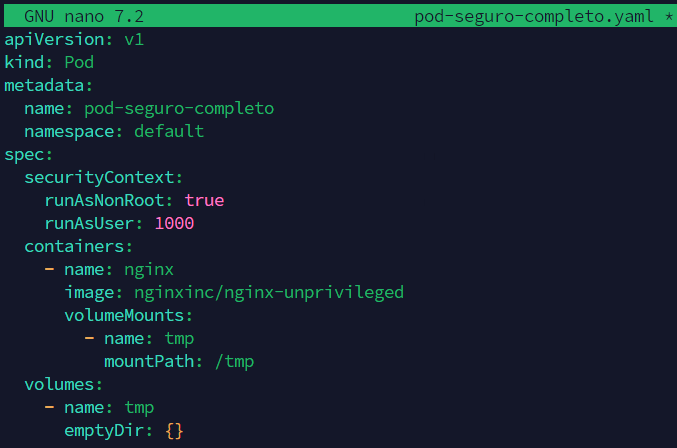
\includegraphics[width=0.65\linewidth]{kyverno/pod-seguro-completo.png}
\caption{Minimal pod manifest used in the integral test}
\label{fig:pod-seguro-yaml}
\end{figure}

\vspace{-\parskip}

After deployment, pod inspection via \texttt{kubectl get pod pod-seguro-completo -o yaml} returns the complete object as persisted in etcd after passing through Kyverno's webhooks. Figures~\ref{fig:test10-1} and~\ref{fig:test10-2} show the result.

\begin{figure}[H]
\centering
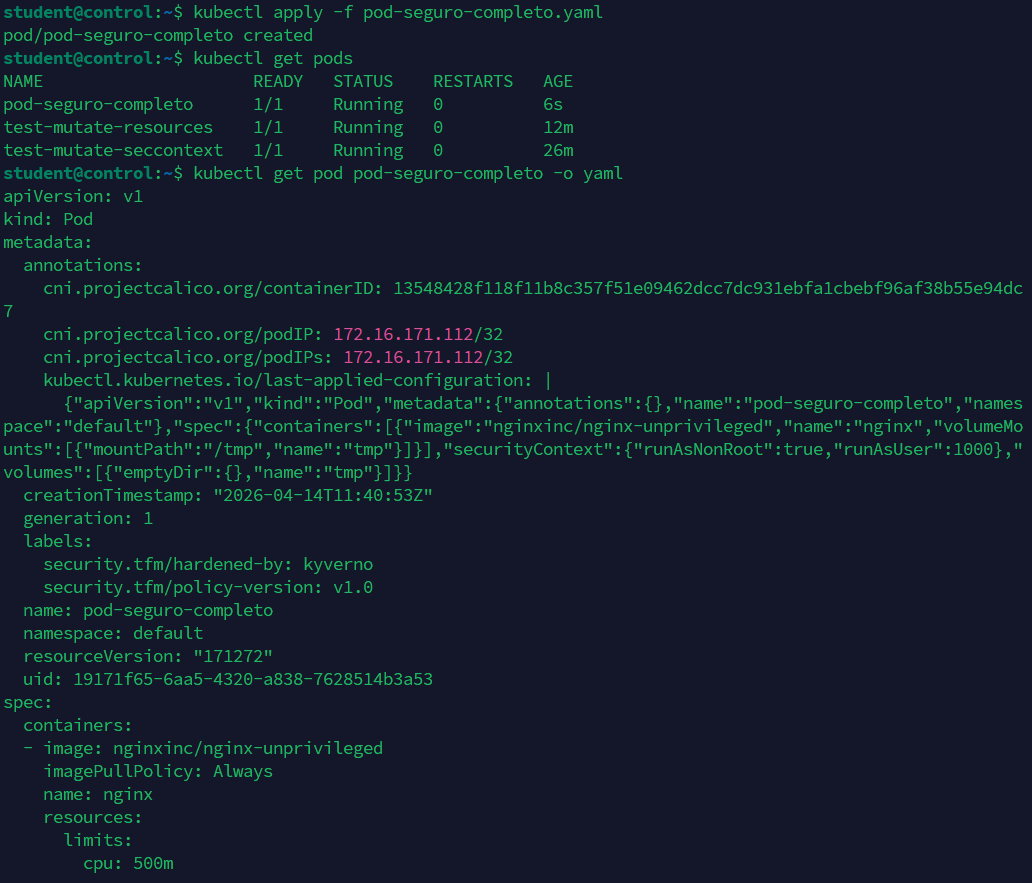
\includegraphics[width=0.95\linewidth]{kyverno/test10-1.png}
\caption{Integral test (part 1): pod metadata and resources after admission}
\label{fig:test10-1}
\end{figure}

\vspace{-\parskip}

\begin{figure}[H]
\centering
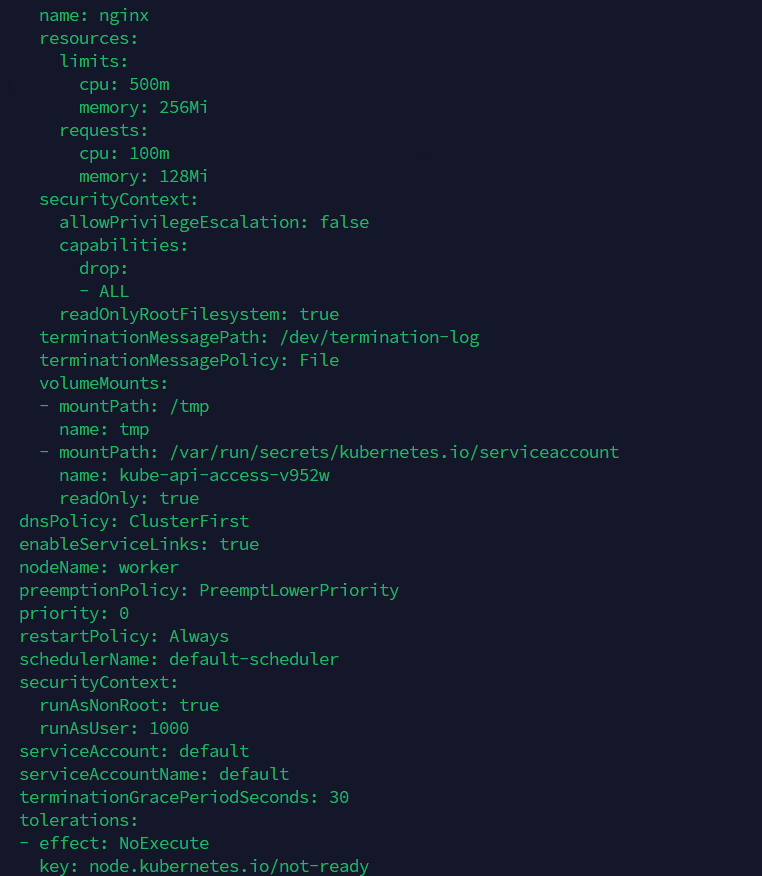
\includegraphics[width=0.85\linewidth]{kyverno/test10-2.png}
\caption{Integral test (part 2): complete security profile injected by Kyverno}
\label{fig:test10-2}
\end{figure}


The analysis of the persisted object confirms the presence of all fields injected by the four active mutation policies: \texttt{resources.requests} and \texttt{resources.limits} (P4); \texttt{allow\-Privilege\-Escalation:\,false} and \texttt{capabilities.drop:\,[ALL]} (P5); \texttt{readOnly\-Root\-Filesystem:\,true} (P6); and labels \texttt{security.tfm/\allowbreak{}hardened-by:\,kyverno} and \texttt{security.tfm/\allowbreak{}policy-version:\,v1.0} (P7). Calico annotations additionally confirm that the pod has been assigned IP \texttt{172.16.171.112} in CIDR \texttt{172.16.0.0/16} and scheduled on the \texttt{worker} node.

This test constitutes the direct empirical evidence of the work's central thesis: a developer can define a pod with the minimum fields necessary for its function and obtain, in a completely transparent manner, a correctly secured pod that complies with the security profile defined by the organisation.

\subsection{The mutation-validation order verified empirically}

During testing, a behaviour was observed that empirically illustrates the webhook execution order described theoretically in Section~5.3.2. When attempting to deploy a pod with \texttt{allow\-Privilege\-Escalation:\,true} declared explicitly while both P5 and P2 were simultaneously active, the pod was created successfully despite P2 operating in \texttt{Enforce} mode.

The cause is precise: P5 (\textit{mutating webhook}) executed before P2 (\textit{validating webhook}) and overwrote the \texttt{true} value declared in the manifest with \texttt{false}, so that when P2 evaluated the resource, it already contained the compliant value. The \texttt{patch\-Strategic\-Merge} of P5 overwrites the field even when the developer has explicitly declared it with an insecure value.

This behaviour was verified by temporarily disabling P5 and applying the same pod: in the absence of mutation, P2 correctly rejected the request. Upon restoring P5, the pod was again admitted with the mutated value. This experiment empirically confirms that, in the adopted design, mutation has \textit{absolute precedence} over validation, and that validation policies complement but do not replace mutation policies as the primary security mechanism.

% ─────────────────────────────────────────────
\section{Policy Reports: compliance auditing}
% ─────────────────────────────────────────────

Kyverno's Reports Controller automatically generates \texttt{PolicyReport} resources (namespace-scoped) and \texttt{ClusterPolicyReport} resources (cluster-scoped) that consolidate the results of evaluating all policies over all system resources. These reports constitute the native compliance audit mechanism and allow centrally answering the question: which cluster resources comply with the security policies?

Figure~\ref{fig:clusterpolicyreports} shows the \texttt{ClusterPolicyReport} generated for the \texttt{test-networkpolicy} namespace: the \texttt{Namespace} type resource has passed the P8 evaluation, with result 1~PASS and 0~FAIL.

\begin{figure}[htbp]
\centering
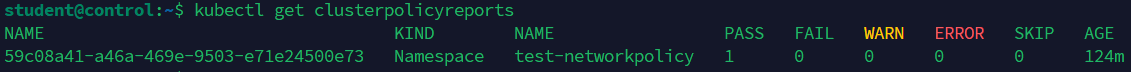
\includegraphics[width=0.95\linewidth]{kyverno/kubectl get clusterpolicyreports.png}
\caption{ClusterPolicyReport: evaluation of the generation policy on the test namespace}
\label{fig:clusterpolicyreports}
\end{figure}

Figure~\ref{fig:policyreports} shows the \texttt{PolicyReport} objects for the \texttt{default} namespace, one per active pod. The three pods --- \texttt{pod-seguro-completo}, \texttt{test-mutate-resources} and \texttt{test-mutate-sec\-context} --- record 7~PASS and 0~FAIL.

\begin{figure}[htbp]
\centering
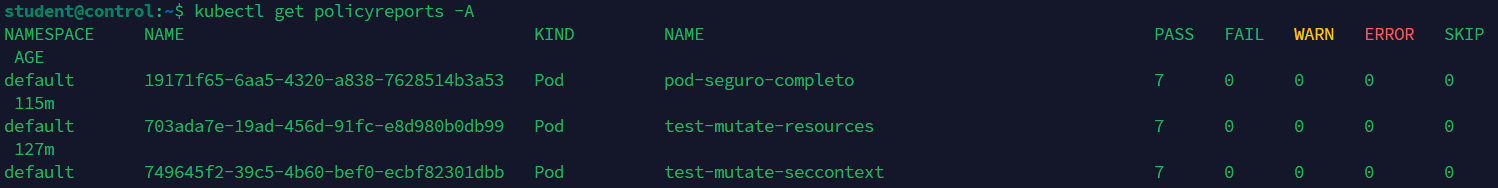
\includegraphics[width=0.95\linewidth]{kyverno/kubectl get policyreports -A.png}
\caption{PolicyReports of the \texttt{default} namespace: 7 PASS per pod, 0 violations}
\label{fig:policyreports}
\end{figure}

The value 7 corresponds exactly to the number of policies that evaluate \texttt{Pod} type resources (P1 to P7). Policy P8 does not appear in these reports because its scope covers \texttt{Namespace} type resources, and its results are reflected in the \texttt{ClusterPolicyReport} objects of Figure~\ref{fig:clusterpolicyreports}. These reports demonstrate that the implemented system not only acts at admission time, but also provides continuous visibility into the cluster's compliance state --- a fundamental requirement in DevSecOps environments oriented towards auditing and regulatory compliance.

\chapter{GitOps Integration with ArgoCD}

This chapter documents the implementation of the Continuous Deployment layer of the DevSecOps environment, materialised through ArgoCD as the GitOps controller. Up to this point, Kyverno policies have been managed via direct \texttt{kubectl apply}, which implies that the cluster state and the state declared in the manifests are not continuously linked: any manual modification in the cluster can diverge from the desired state without any mechanism detecting or correcting it. This chapter implements the continuous synchronisation plane announced in Section~5.1, closing the DevSecOps architecture with the layer that connects the Git repository as the single source of truth with the real state of the cluster.

The chapter is organised into six sections. The first describes the GitOps repository design and the decision on its structure. The second documents ArgoCD's deployment in the cluster, including a relevant technical incident during installation. The third covers the creation of the \texttt{Application} that places Kyverno policies under declarative management, and the fourth documents a technical finding about the friction between defaults injected by Kyverno and ArgoCD's comparison engine. The fifth section collects three \textit{drift protection} tests that empirically demonstrate the ArgoCD\,+\,Kyverno complementarity thesis of Chapter~5. The sixth section extends the GitOps architecture to a real workload, and the chapter concludes with a technical analysis of the interaction between Kyverno's \textit{mutating webhooks} and ArgoCD's comparison engine, directly addressing the permanent \textit{drift} risk warned about by the official documentation. The integration with the Continuous Integration plane, which will materialise the two-repository pattern described theoretically in Section~5.1, is addressed in Chapter~8 through the incorporation of the GitHub Actions pipeline.

% ─────────────────────────────────────────────
\section{GitOps repository design}
% ─────────────────────────────────────────────

The GitOps repository design requires a prior architectural decision: the number of repositories that will structure the system. Section~5.1 theoretically described the \textit{two-repository pattern} ---one for application source code and another for Kubernetes configuration--- as the usual solution in production environments. Within the scope of this chapter, where the Continuous Integration pipeline has not yet been incorporated, a single repository is used ---called \texttt{tfm-gitops}--- which contains the Kyverno policies and demo application manifests, organised using folders that preserve the conceptual separation between planes. This structure will be expanded in Chapter~8 with the introduction of the second repository (\texttt{tfm-demo-app}), which will host the application source code and Dockerfile. The Continuous Integration pipeline will build the image from that second repository and update the image tag in \texttt{tfm-gitops}, materialising the complete two-repository pattern announced in the architecture.

The final repository structure, visible in Figure~\ref{fig:repo-estructura}, reflects three independent functional planes:

\begin{figure}[htbp]
\centering
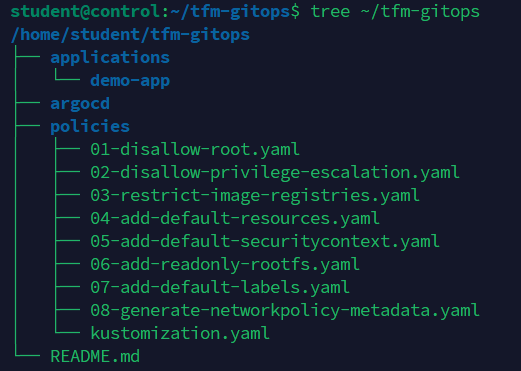
\includegraphics[width=0.70\linewidth]{actions/bloque1_estructuraInicial.png}
\caption{Structure of the \texttt{tfm-gitops} repository with separation by functional planes}
\label{fig:repo-estructura}
\end{figure}

\begin{itemize}
  \item \texttt{policies/}: contains the eight \texttt{ClusterPolicy} manifests (P1--P8) and the \texttt{kustomization.yaml} file that groups them.
  \item \texttt{applications/demo-app/}: contains the demonstrative workload manifests (Namespace, Deployment, Service) and their own \texttt{kustomization.yaml}.
  \item \texttt{argocd/}: contains \texttt{Application} type manifests that define how ArgoCD should manage each of the previous planes.
\end{itemize}

The \texttt{kustomization.yaml} file in the \texttt{policies/} folder plays a central role in the ArgoCD integration. Kustomize \cite{kustomize_docs} is a native Kubernetes grouping mechanism that ArgoCD recognises automatically: when pointing an \texttt{Application} to a directory containing a \texttt{kustomization.yaml}, ArgoCD renders all listed resources and manages them as a logical unit. This avoids the need to individually reference each policy file in the ArgoCD configuration. Figure~\ref{fig:kustomization} shows the file content, listing the eight manifests in sequential order.

\begin{figure}[H]
\centering
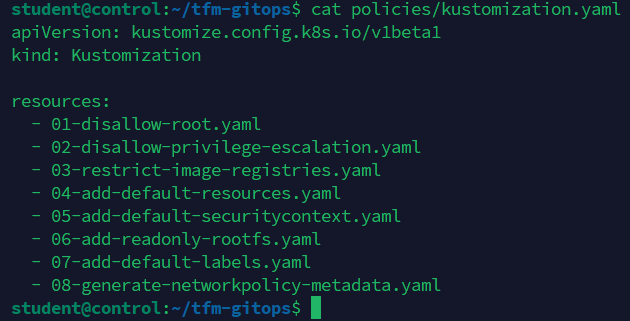
\includegraphics[width=0.75\linewidth]{actions/bloque1_kustomization.png}
\caption{\texttt{kustomization.yaml} file in the \texttt{policies/} folder with all eight policies}
\label{fig:kustomization}
\end{figure}

% ─────────────────────────────────────────────
\section{ArgoCD deployment}
% ─────────────────────────────────────────────

ArgoCD is installed in the cluster by applying the official manifests in the dedicated namespace \texttt{argocd}:

\begin{lstlisting}
kubectl create namespace argocd
kubectl apply -n argocd -f https://raw.githubusercontent.com/argoproj/argo-cd/stable/manifests/install.yaml
\end{lstlisting}

\subsection{Incident during installation: annotation size limit on CRDs}

During the first execution of the above command, an error occurred that prevented the registration of the \texttt{ApplicationSet} CRD:

\begin{lstlisting}
The ApplicationSet "applicationsets.argoproj.io" is invalid:
metadata.annotations: Too long: may not be more than 262144 bytes
\end{lstlisting}

The root cause of this error lies in the \textit{client-side apply} mechanism used by default by \texttt{kubectl apply}: when applying a resource, \texttt{kubectl} serialises the complete manifest and stores it in the annotation \texttt{kubectl.kubernetes.io/\allowbreak{}last-applied-configuration} of the object. The OpenAPI schema of the \texttt{ApplicationSet} CRD exceeds the 256~KB limit imposed by Kubernetes for an individual annotation value, making it impossible to complete the operation through the standard mechanism.

The solution is to reinstall the manifests using \textit{server-side apply} \cite{kubernetes_ssa}, which delegates the \textit{merge} logic to the API Server instead of storing it in the client annotation:

\begin{lstlisting}
kubectl apply -n argocd \
  -f https://raw.githubusercontent.com/argoproj/argo-cd/stable/manifests/install.yaml \
  --server-side --force-conflicts
\end{lstlisting}

The \texttt{-{}-force-conflicts} flag is necessary because some manifest fields may have ended up in an inconsistent \textit{field manager} state after the first partially completed attempt. With \textit{server-side apply}, the \texttt{last-applied-configuration} field is not used and the CRD is correctly registered regardless of the size of its schema.

\subsection{Deployment verification}

After reinstallation, verification of pod state in the \texttt{argocd} namespace confirms that ArgoCD's seven components are active, as shown in Figure~\ref{fig:argo-pods}.

\begin{figure}[H]
\centering
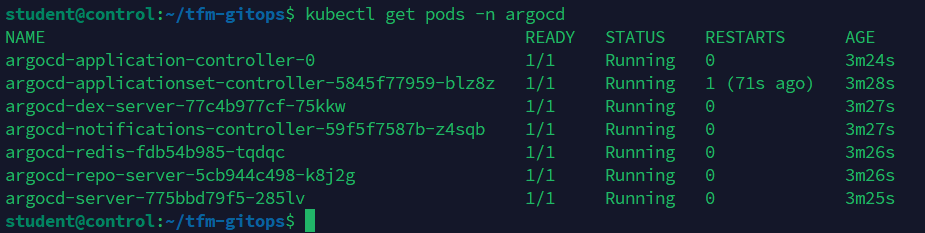
\includegraphics[width=0.95\linewidth]{actions/bloque2_verificaionPodsArgo.png}
\caption{ArgoCD's seven components in \texttt{Running} state in the \texttt{argocd} namespace}
\label{fig:argo-pods}
\end{figure}

The seven pods correspond to the components described in Section~5.2.3: \texttt{application-cont\-roller} (continuous cluster state reconciliation), \texttt{applicationset-controller} (generation of \texttt{Application} objects from templates), \texttt{dex-server} (federated authentication), \texttt{notifications-controller} (alerts and notifications), \texttt{redis} (internal state cache), \texttt{repo-server} (Git repository cloning and rendering) and \texttt{server} (ArgoCD API and UI).

Verification of registered CRDs confirms that the three ArgoCD resource types are available in the cluster, as seen in Figure~\ref{fig:argo-crds}.

\begin{figure}[H]
\centering
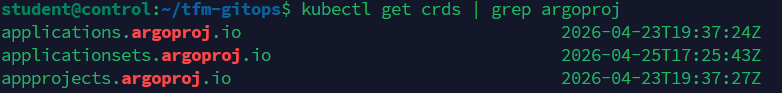
\includegraphics[width=0.85\linewidth]{actions/bloque2_CRDSregistrados.png}
\caption{ArgoCD CRDs registered in the cluster: \texttt{applications}, \texttt{applicationsets} and \texttt{appprojects}}
\label{fig:argo-crds}
\end{figure}

The ArgoCD dashboard (version~3.3.8) is accessible through port \texttt{8080} of the control node via exposure of the \texttt{argocd-server} service. Figure~\ref{fig:argo-dashboard} shows the initial interface state before registering any \texttt{Application}.

\begin{figure}[htbp]
\centering
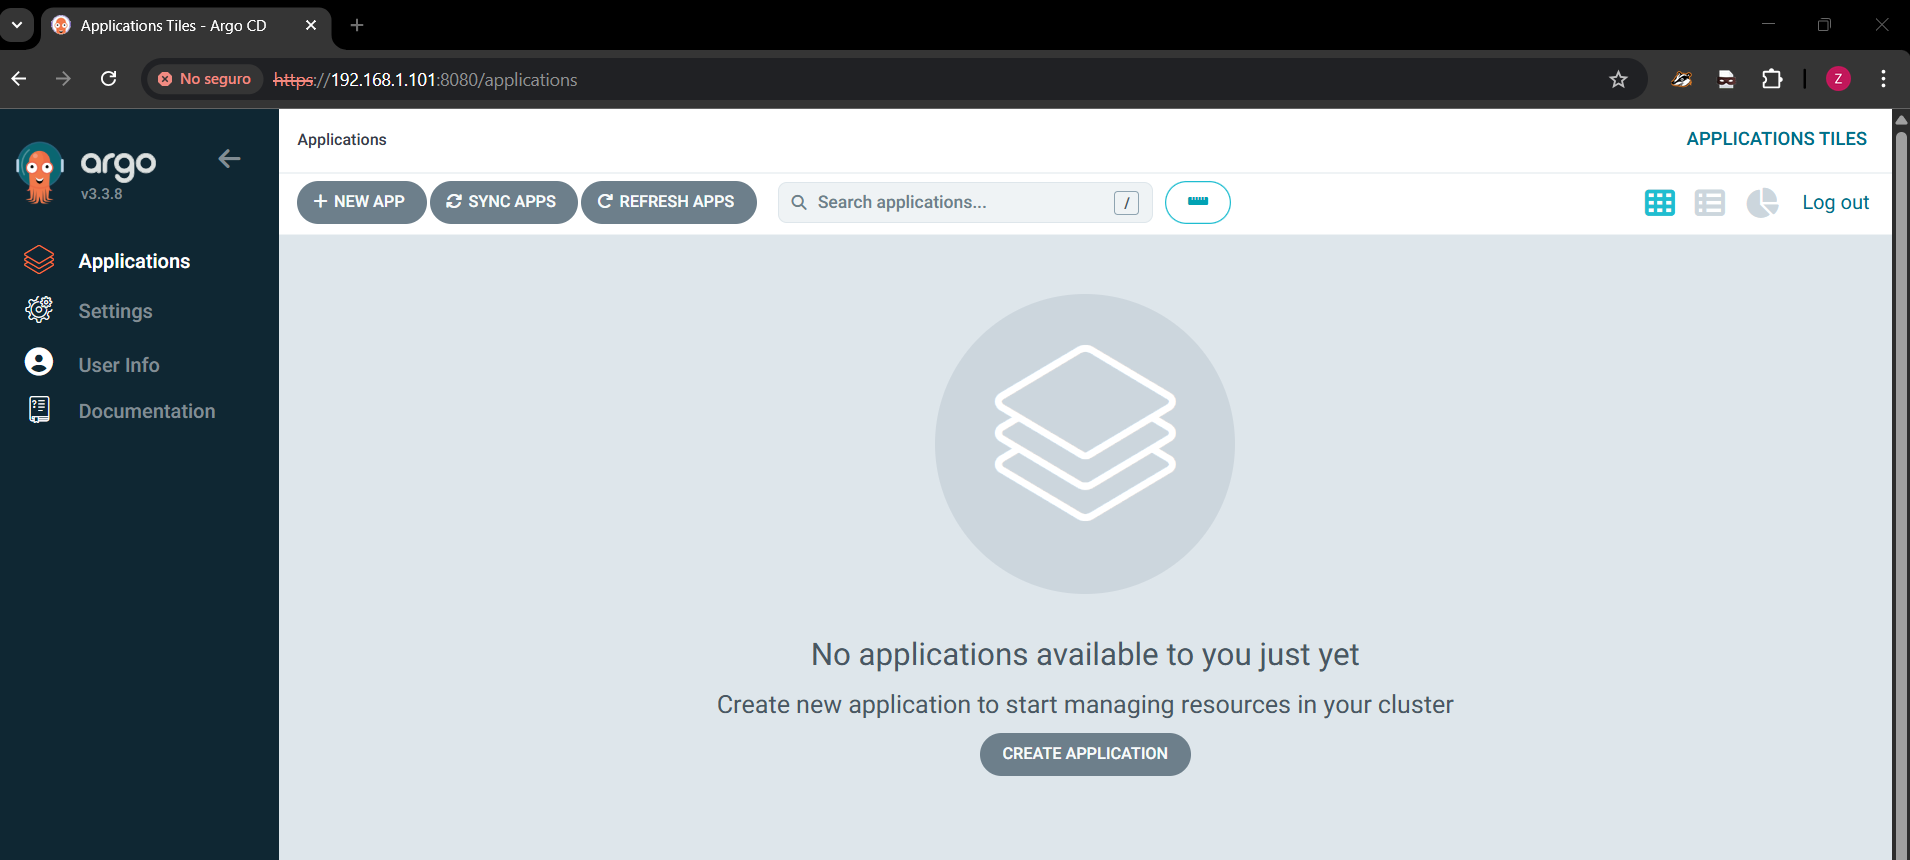
\includegraphics[width=0.95\linewidth]{actions/bloque2_dashboard.png}
\caption{ArgoCD v3.3.8 interface accessible at \texttt{https://192.168.1.101:8080}}
\label{fig:argo-dashboard}
\end{figure}

% ─────────────────────────────────────────────
\section{Application for Kyverno policies}
\label{sec:app-policies}
% ─────────────────────────────────────────────

An \texttt{Application} is ArgoCD's central CRD \cite{argocd_docs}: it represents the minimum unit of declarative management and encapsulates three elements ---the Git source of the manifests, the destination in the cluster where they should be deployed and the synchronisation policy that defines how and when to synchronise. The manifest \texttt{app-policies.yaml}, shown in Figure~\ref{fig:app-policies-yaml}, defines the \texttt{Application} that places the eight Kyverno policies under GitOps management.

\begin{figure}[H]
\centering
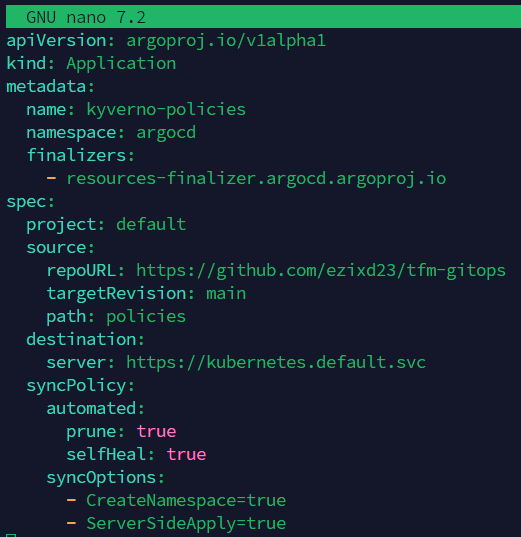
\includegraphics[width=0.70\linewidth]{actions/bloque3_app-policies.png}
\caption{Manifest \texttt{app-policies.yaml}: Application managing Kyverno's ClusterPolicies}
\label{fig:app-policies-yaml}
\end{figure}
\vspace{-\parskip}

Each manifest field responds to a justified technical decision:

\begin{itemize}
  \item \texttt{finalizers: resources-finalizer.\allowbreak{}argocd.argoproj.io}: activates \textit{cascade delete}, so that when the ArgoCD \texttt{Application} is deleted, the synchronised resources in the cluster are also deleted. Guarantees that no orphan policies remain if the \texttt{Application} is removed.
  \item \texttt{automated.prune:\,true}: enables the automatic deletion of resources that exist in the cluster but have been removed from Git. Without this field, ArgoCD would detect the divergence but would not act, requiring manual intervention.
  \item \texttt{automated.selfHeal:\,true}: activates the automatic detection and reversal of manual modifications made directly on cluster resources. This field is the heart of the complementarity thesis with Kyverno formulated in Section~5.2.3: while Kyverno protects generated resources (NetworkPolicies), ArgoCD protects the very sources of that generation (ClusterPolicies).
  \item \texttt{syncOptions.ServerSideApply:\,true}: delegates resource \textit{merge} to the API Server, avoiding the annotation size problem described in the previous section and being consistent with the installation of ArgoCD's own manifests.
  \item \texttt{syncOptions.CreateNamespace:\,true}: allows ArgoCD to create the destination namespace if it does not exist, although in this case the \texttt{kyverno} namespace was already created by Kyverno's prior installation.
\end{itemize}

\subsection{Deployment and synchronisation process}

Before applying the \texttt{Application}, the policies previously deployed via direct \texttt{kubectl apply} are removed from the cluster, so that the subsequent deployment unequivocally demonstrates that ArgoCD is the sole provisioning source:

\begin{lstlisting}
kubectl delete clusterpolicies --all
kubectl apply -f ~/tfm-gitops/argocd/app-policies.yaml
\end{lstlisting}

Figure~\ref{fig:app-policies-sync} shows the observed sequence of states: immediately after the manifest is applied, the \texttt{Application} \texttt{kyverno-policies} appears in \texttt{OutOfSync}~+~\texttt{Healthy} state, indicating that ArgoCD has detected the divergence between the repository (which contains the eight policies) and the cluster (which at that moment has none). In the next reconciliation cycle, ArgoCD synchronises the state and the \texttt{Application} transitions to \texttt{Synced}~+~\texttt{Healthy}.

\begin{figure}[H]
\centering
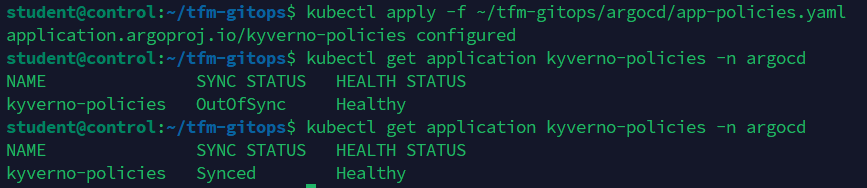
\includegraphics[width=0.95\linewidth]{actions/bloque3_aplicacionEstado.png}
\caption{State transition \texttt{OutOfSync} \textrightarrow{} \texttt{Synced} after first deployment of \texttt{kyverno-policies}}
\label{fig:app-policies-sync}
\end{figure}

Verification that the eight policies have been restored and are managed by ArgoCD is carried out in two steps. The first confirms the \texttt{Ready} state of the eight \texttt{ClusterPolicies}, as shown in Figure~\ref{fig:policies-regeneradas}.

\begin{figure}[H]
\centering
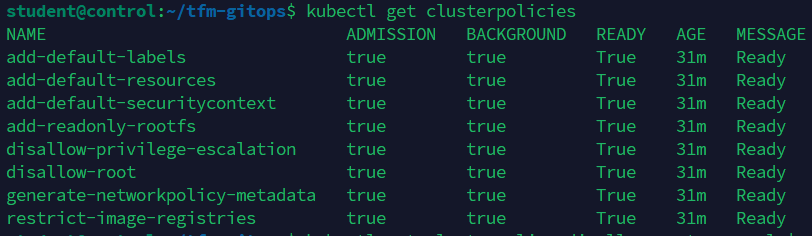
\includegraphics[width=0.95\linewidth]{actions/bloque3_policiesGeneradasDeNuevo.png}
\caption{The eight ClusterPolicies restored by ArgoCD in \texttt{Ready} state}
\label{fig:policies-regeneradas}
\end{figure}
\vspace{-\parskip}

\begin{sloppypar}
The second step verifies that the \textit{ownership} of each policy is established through ArgoCD's traceability annotation. Figure~\ref{fig:argo-anotacion} shows that the \texttt{disallow-root} policy contains the annotation \path{argocd.argoproj.io/tracking-id:kyverno-policies:kyverno.io/ClusterPolicy:/disallow-root}, which unequivocally establishes that this resource is managed by the \texttt{Application} \texttt{kyverno-policies}.
\end{sloppypar}

\begin{figure}[H]
\centering
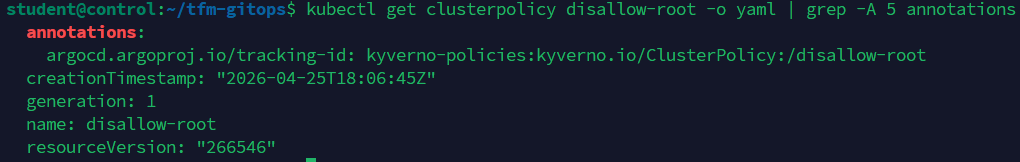
\includegraphics[width=0.95\linewidth]{actions/bloque3_anotacionesArgoCD.png}
\caption{ArgoCD \textit{ownership} annotation in the \texttt{disallow-root} ClusterPolicy}
\label{fig:argo-anotacion}
\end{figure}
\vspace{-\parskip}

ArgoCD's graphical interface, shown in Figure~\ref{fig:argo-arbol}, presents the tree of synchronised resources: the \texttt{Application} \texttt{kyverno-policies} with its eight dependent \texttt{ClusterPolicy} objects, all in \texttt{Synced} state. The commit associated with the last successful synchronisation is visible in the status panel, confirming that the Git repository is the source of truth.

\begin{figure}[H]
\centering
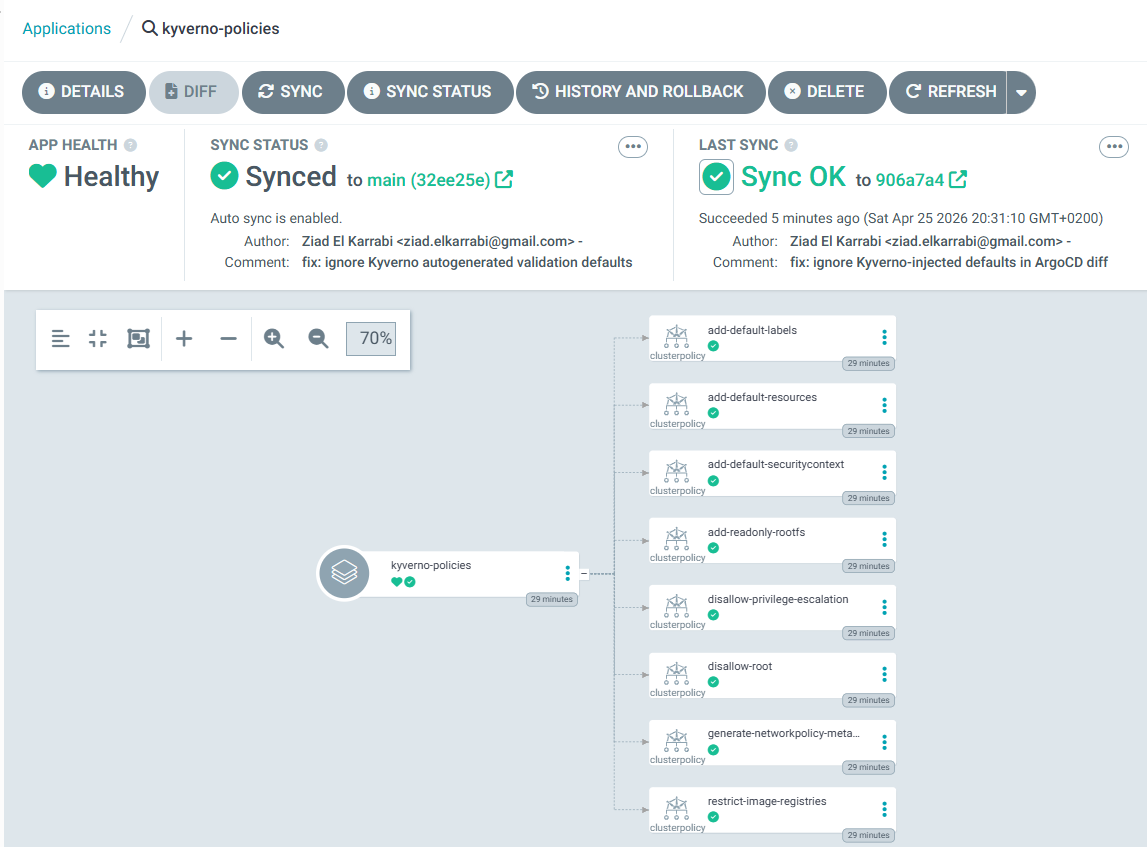
\includegraphics[width=0.95\linewidth]{actions/bloque3_arbolPolicies.png}
\caption{Tree view in ArgoCD: eight ClusterPolicies synchronised from the Git repository}
\label{fig:argo-arbol}
\end{figure}
\vspace{-\parskip}

The end-to-end functional test, shown in Figure~\ref{fig:pod-bloqueado-argo}, confirms that the policies managed by ArgoCD are functionally equivalent to those deployed manually: the attempt to create a pod without \texttt{runAsNonRoot} is rejected by Kyverno's webhook with the same message as in Chapter~6 tests.

\begin{figure}[H]
\centering
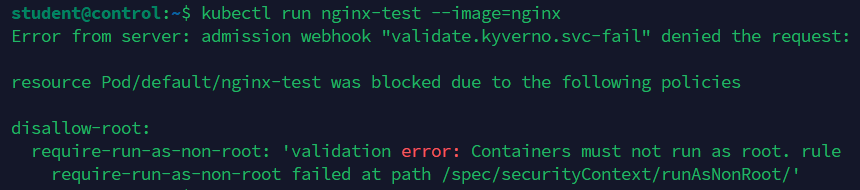
\includegraphics[width=0.90\linewidth]{actions/bloque3_podBloqueado.png}
\caption{End-to-end verification: insecure pod blocked by ArgoCD-managed policies}
\label{fig:pod-bloqueado-argo}
\end{figure}
\vspace{-\parskip}

% ─────────────────────────────────────────────
\section{Managing false drift from Kyverno defaults}
\label{sec:ignore-differences}
% ─────────────────────────────────────────────

After the first successful deployment of the \texttt{Application} \texttt{kyverno-policies}, an unexpected behaviour was observed: the \texttt{Application} periodically reverted to \texttt{OutOfSync} state despite no changes having been made either in Git or in the cluster. Analysis of the ArgoCD diff revealed the root cause: Kyverno itself applies a \textit{mutating webhook} on \texttt{ClusterPolicy} type resources at admission time, injecting default values into fields not specified in the Git manifests. Affected fields include \texttt{spec.\allowbreak{}validationFailureAction} (when not explicitly declared in some policy), \texttt{spec.\allowbreak{}rules[*].skipBackgroundRequests} and \texttt{spec.\allowbreak{}rules[*].allowExistingViolations}.

This situation is an example of what ArgoCD's documentation calls \textit{false drift} \cite{argocd_diffing}: the state in the cluster differs from the state in Git, but the difference is not the result of an unauthorised modification but of internal system behaviour. From ArgoCD's perspective, the resource in the cluster has additional fields or fields with different values than those declared in Git, which triggers the \texttt{selfHeal} mechanism unnecessarily, creating an unstable reconciliation loop.

\subsection{Evaluation of resolution options}

In this situation there are two resolution strategies:

\begin{enumerate}
  \item \textbf{Add default values to the manifests in Git}: explicitly declare in each manifest the fields that Kyverno injects, so that the Git state and the cluster state match exactly.
  \item \textbf{Configure \texttt{ignoreDifferences} in the \texttt{Application}}: instruct ArgoCD to ignore certain fields when performing the comparison, preserving the Git manifests in their minimal form.
\end{enumerate}

The first option has a significant operational disadvantage: the default values injected by Kyverno are version-dependent. A Kyverno update that changes existing defaults or adds new fields would require updating all Git manifests synchronously, creating an unnecessary coupling between the engine version and the policy manifests. This dependency violates the separation of responsibilities principle underlying the GitOps pattern: Git should contain the operator's \textit{intent}, not an exact mirror of the system's internal state.

The second option, \texttt{ignoreDifferences} \cite{argocd_diffing}, allows expressing exactly this distinction: the ignored fields are internal management fields of the engine, not attributes of the policy declared by the operator. This strategy is adopted by adding the following block to the \texttt{app-policies.yaml} manifest:

\begin{lstlisting}
ignoreDifferences:
- group: kyverno.io
  kind: ClusterPolicy
  jqPathExpressions:
  - .spec.rules[] | .skipBackgroundRequests
  - .spec.rules[] | .allowExistingViolations
  - .spec.rules[] | .validate? | .allowExistingViolations?
  - .spec.validationFailureAction
\end{lstlisting}

The \texttt{jqPathExpressions} use \texttt{jq} syntax to reference fields that should be excluded from comparison. The use of \texttt{?.} in \texttt{.validate?} avoids errors in \textit{mutate} or \textit{generate} rules where the \texttt{validate} field does not exist. After applying this configuration and re-synchronising, the \texttt{Application} remains stably in \texttt{Synced}~+~\texttt{Healthy} state, confirmed by the commit ``fix: ignore Kyverno-injected defaults in ArgoCD diff'' visible in the last synchronisation panel of Figure~\ref{fig:argo-arbol}.

% ─────────────────────────────────────────────
\section{Drift protection tests}
% ─────────────────────────────────────────────

With the \texttt{Application} \texttt{kyverno-policies} stable, three tests are executed that empirically demonstrate the complementarity between ArgoCD and Kyverno as \textit{drift protection} mechanisms at different architectural planes. Kyverno's mechanism, documented in Section~6.5 of the previous chapter, protects the resources \textit{generated} by the policies (NetworkPolicies). ArgoCD's mechanism documented below protects the source policies themselves.

\subsection{Self-healing upon manual modification}

The first test simulates an internal actor --- a cluster administrator with direct \texttt{kubectl} access --- modifying a policy to weaken security controls. The scenario is realistic: in an environment without GitOps, this modification would be permanent and might go unnoticed. With ArgoCD and \texttt{selfHeal:\,true}, the cluster automatically reconciles with the Git declarative state.

The test modifies the \texttt{message} field of the \texttt{disallow-root} policy via \texttt{kubectl edit}, replacing the original text with the marker \texttt{DRIFT TEST - manually modified message}. Although modifying the error message does not affect validation logic, the change is sufficient for ArgoCD to detect the divergence. Figure~\ref{fig:prueba1-modificacion} shows two consecutive queries: the first confirms that the modification was correctly applied (the mutated message appears in the three contexts generated by autogen); the second, executed moments later, shows that the message has returned to the original value \texttt{Containers must not run as root}, confirming that ArgoCD has reverted the change.

\begin{figure}[H]
\centering
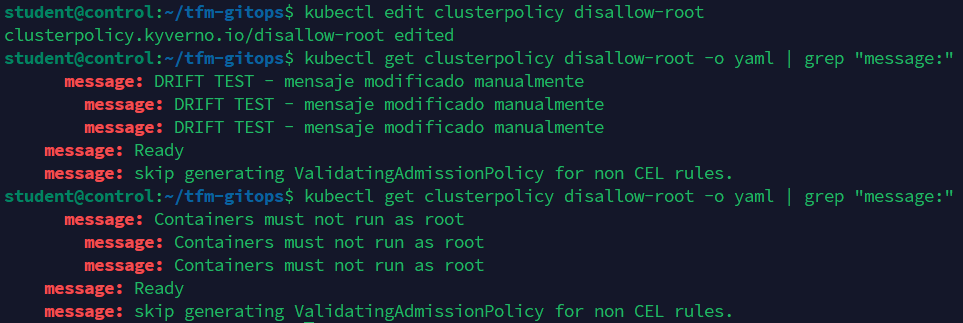
\includegraphics[width=0.95\linewidth]{actions/bloque4_prueba1ModificadoPolicy.png}
\caption{Test 1: manual modification reverted by ArgoCD via \texttt{selfHeal}}
\label{fig:prueba1-modificacion}
\end{figure}

In this experiment, the reversal occurred within seconds. Although the Git repository \textit{polling} interval is configured by default to 3~minutes, ArgoCD maintains in parallel a continuous \textit{watch} over synchronised resources via the Kubernetes API, allowing it to detect cluster changes almost in real time and initiate the reconciliation cycle immediately without waiting for the next Git \textit{polling} cycle.

\subsection{Policy deployment via Git commit}

The second test demonstrates the GitOps flow in the downstream direction: Git as a provisioning mechanism without direct cluster access. A new policy, \texttt{disallow-latest-tag}, is created that rejects pods whose images are tagged with \texttt{:latest} --- a practice that prevents deployment reproducibility by referring to an image whose content can change without notice. The policy is created directly in the repository's \texttt{policies/} directory, referenced in \texttt{kustomization.yaml} and uploaded via commit and push to the remote repository.

Figure~\ref{fig:prueba2-commit} shows the complete process: file creation, \texttt{kustomiza\-tion.yaml} modification, commit and push. The commit message, \texttt{feat: add disallow-latest-tag policy in kustomization.yaml}, documents the change's intent.

\begin{figure}[H]
\centering
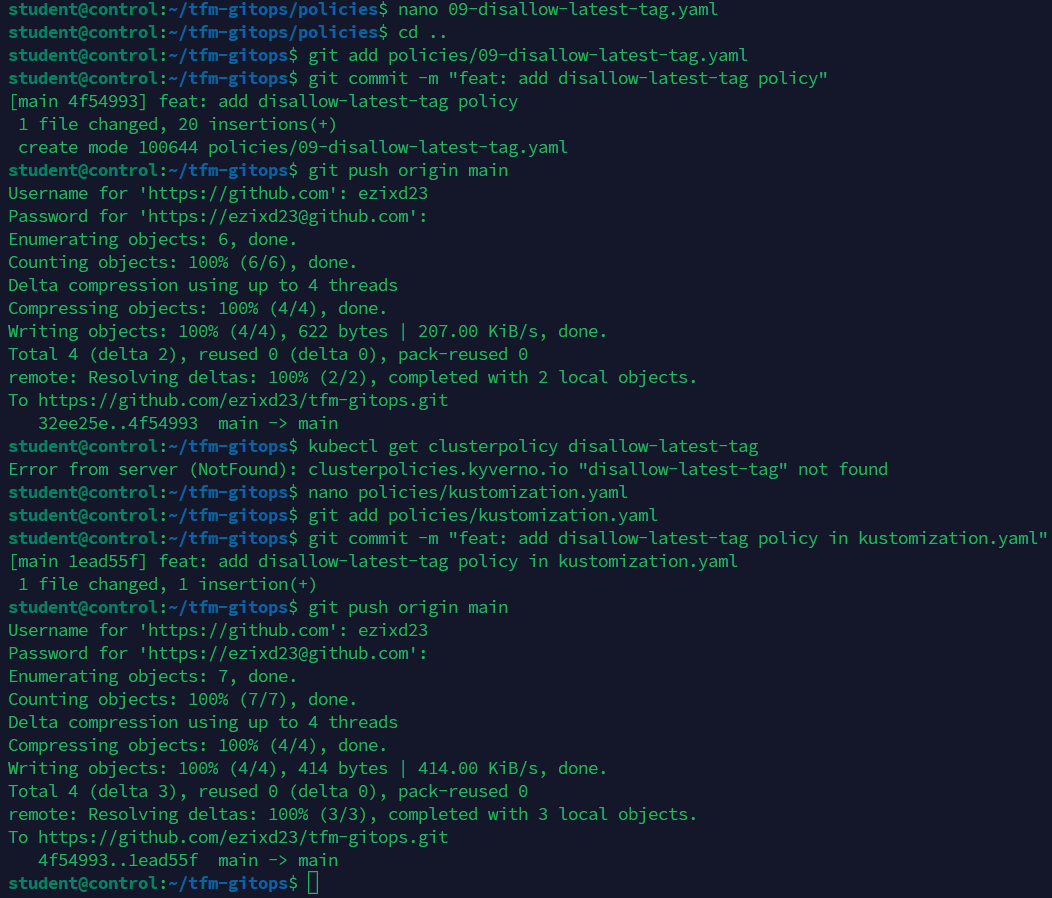
\includegraphics[width=0.95\linewidth]{actions/bloque4_prueba2CreacionyCommitNuevaPolicy.png}
\caption{Test 2: new policy created via Git commit}
\label{fig:prueba2-commit}
\end{figure}
\vspace{-\parskip}

Figure~\ref{fig:prueba2-desplegada} confirms that the \texttt{disallow-latest-tag} policy has been deployed in the cluster by ArgoCD without any direct intervention, with an age of 2~minutes and 42~seconds compared to the other policies that have been active for over an hour. The \texttt{BACKGROUND:\,false} field reflects that this policy, due to its exclusion condition-based design, does not generate retroactive evaluations on existing pods.

\begin{figure}[H]
\centering
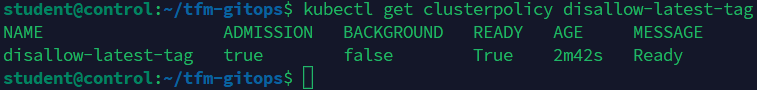
\includegraphics[width=0.90\linewidth]{actions/bloque4_prueb2PolicyDesplegada.png}
\caption{Test 2: \texttt{disallow-latest-tag} automatically deployed by ArgoCD (2m42s age)}
\label{fig:prueba2-desplegada}
\end{figure}
\vspace{-\parskip}

ArgoCD's interface, shown in Figure~\ref{fig:prueba2-ui}, reflects the updated tree with nine \texttt{ClusterPolicies} --- the new policy appears as an additional node in the graph with a timestamp of 2~minutes ago, while the rest has been synchronised for over an hour.

\begin{figure}[H]
\centering
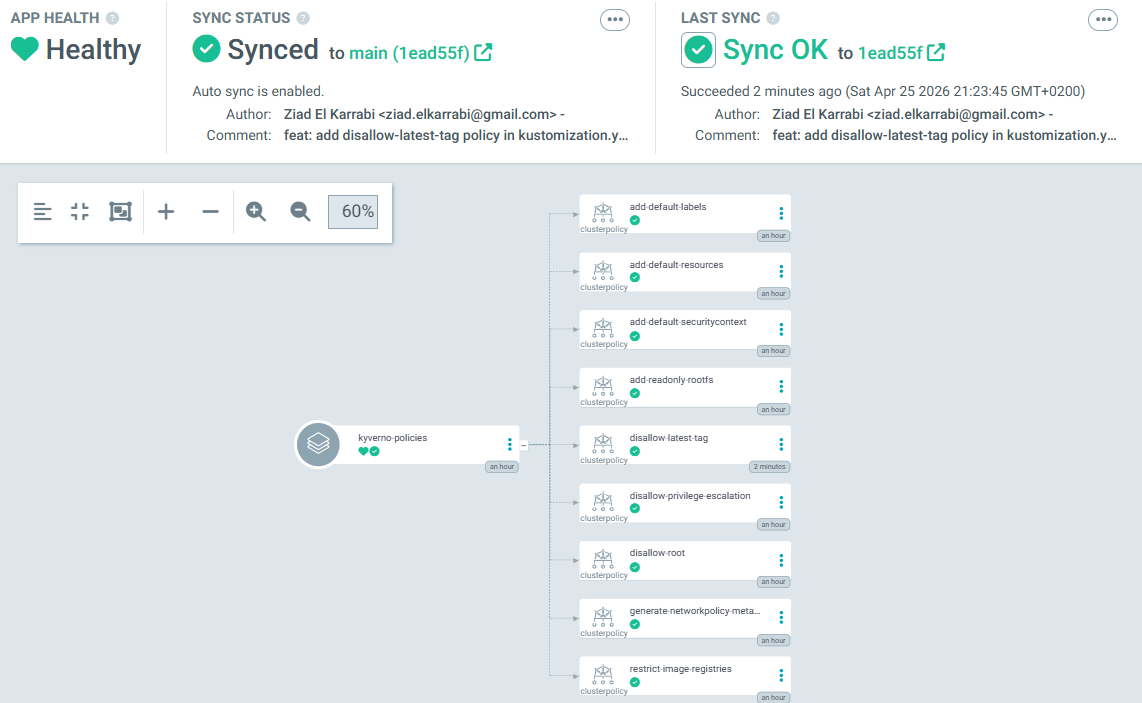
\includegraphics[width=0.95\linewidth]{actions/bloque4_prueba2AparicionUI.png}
\caption{Test 2: ArgoCD tree updated with the new \texttt{disallow-latest-tag} policy}
\label{fig:prueba2-ui}
\end{figure}
\vspace{-\parskip}

\subsection{Protection against deletion}

The third test verifies that ArgoCD automatically restores a policy deleted directly from the cluster. This scenario complements the Kyverno \textit{drift protection} test documented in Section~6.5, where it was demonstrated that the Background Controller restores the \texttt{block-cloud-metadata} NetworkPolicy generated by P8. In this case, the deletion affects the source policy that generates it.

The \texttt{disallow-root} policy is deleted via \texttt{kubectl delete clusterpolicy\allowbreak disallow-root}. Figure~\ref{fig:prueba3-eliminacion} shows the sequence: the deletion is confirmed with the message \texttt{clusterpolicy.\allowbreak kyverno.\allowbreak io "disallow-root" deleted}; the immediate subsequent query returns an empty result. However, 48~seconds later, a new query shows the policy again in \texttt{Ready} state, with an age of 48~seconds compared to the minutes of the others, confirming that ArgoCD has recreated it.
\begin{figure}[H]
\centering
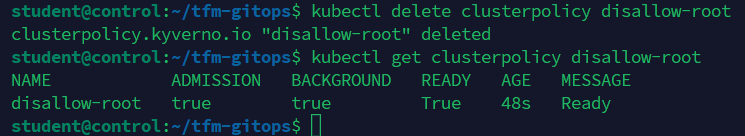
\includegraphics[width=0.90\linewidth]{actions/bloque4_prueba3ProteccionAnteEliminacion.png}
\caption{Test 3: \texttt{disallow-root} policy restored by ArgoCD 48~s after manual deletion}
\label{fig:prueba3-eliminacion}
\end{figure}

The combination of the three tests demonstrates that the system operates with two orthogonal protection layers: ArgoCD guarantees that policies defined in Git always exist and are not modified; Kyverno guarantees that resources generated by those policies (NetworkPolicies) cannot be deleted or modified either. The removal of either protection layer does not completely compromise system security, but does reduce its resilience surface.

% ─────────────────────────────────────────────
\section{Application for the demo workload}
% ─────────────────────────────────────────────

The GitOps architecture implemented up to this point manages only the platform policy plane. To complete the two-plane architecture described in Section~5.1 and demonstrate that the system works in an integrated manner for real workloads, a second \texttt{Application} is implemented that deploys a demo application managed declaratively from the same GitOps repository.

\subsection{Demo application design}

The chosen base image is \texttt{nginxinc/nginx-unprivileged:1.27-alpine}, available on \texttt{docker.io} under the \texttt{nginxinc/} prefix that satisfies policy P3 (\texttt{restrict-image-regist\-ries}). The \textit{unprivileged} variant of the official nginx image is specifically designed to run without root privileges: the nginx process listens on port~8080 instead of port~80 (which would require \texttt{CAP\_NET\_BIND\_SERVICE}) and runs with UID~101, being compatible with policy P1 (\texttt{disallow-root}) without additional configuration.

The demo application manifests are three:

\textbf{Namespace} (\texttt{namespace.yaml}): declares the \texttt{demo-app} namespace with identification labels. The label \texttt{purpose:\,tfm-demo} is relevant because its existence activates policy P8 (\texttt{generate-networkpolicy-metadata}), which will automatically generate the IMDS blocking NetworkPolicy as soon as the namespace is created.

\textbf{Deployment} (\texttt{deployment.yaml}), whose content is shown in Figure~\ref{fig:demo-deployment}: specifies 2~replicas of the \texttt{nginx-unprivileged} image, the pod-level \texttt{securityContext} with \texttt{runAsNonRoot:\,true} and \texttt{runAsUser:\,101}, and three \texttt{emptyDir} volume mounts --- \texttt{/tmp}, \texttt{/var/cache/nginx} and \texttt{/var/run}. The inclusion of these three volumes directly responds to policy P6 (\texttt{add-readonly-rootfs}), which forces the root filesystem to read-only mode: nginx requires writing PID files to \texttt{/var/run}, cache files to \texttt{/var/cache/nginx} and temporary files to \texttt{/tmp}, and without the corresponding volumes the process would fail to start. This configuration materialises the lesson documented in Section~6.4.3: the policy is not weakened, but rather forces the developer to be explicit about their application's write requirements.

\begin{figure}[H]
\centering
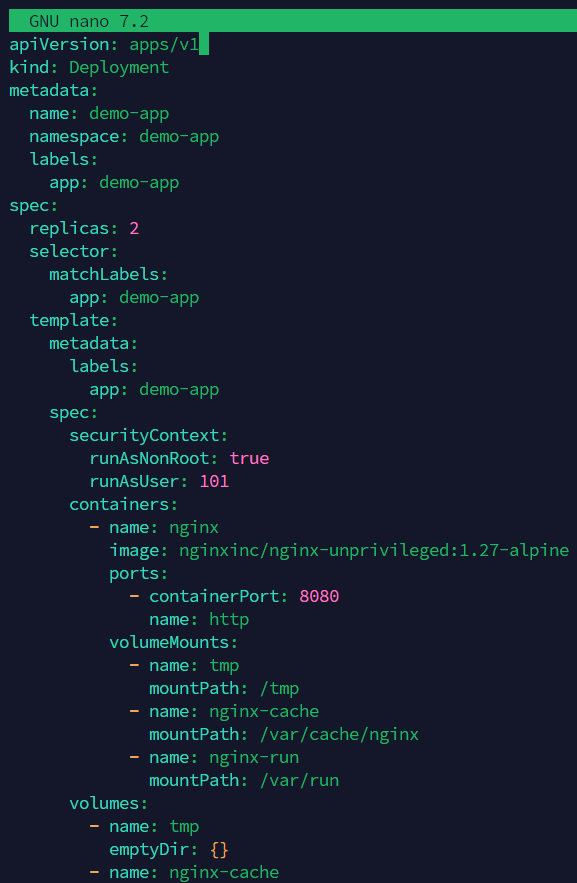
\includegraphics[width=0.70\linewidth]{actions/bloque5_deploymnet.png}
\caption{Demo application \texttt{deployment.yaml} manifest with three \texttt{emptyDir} volumes}
\label{fig:demo-deployment}
\end{figure}
\vspace{-\parskip}

\textbf{Service} (\texttt{service.yaml}): exposes the application via a \texttt{ClusterIP} that maps port~80 to the container's port~8080, with an additional \texttt{NodePort} configured at \texttt{8888} for laboratory access.

\subsection{Application manifest and deployment}

The manifest \texttt{app-demo.yaml}, shown in Figure~\ref{fig:app-demo-yaml}, defines the ArgoCD \texttt{Application} for the workload. There is a deliberate design difference compared to \texttt{app-policies.yaml}: the \texttt{selfHeal} field is configured to \texttt{false}.

\begin{figure}[H]
\centering
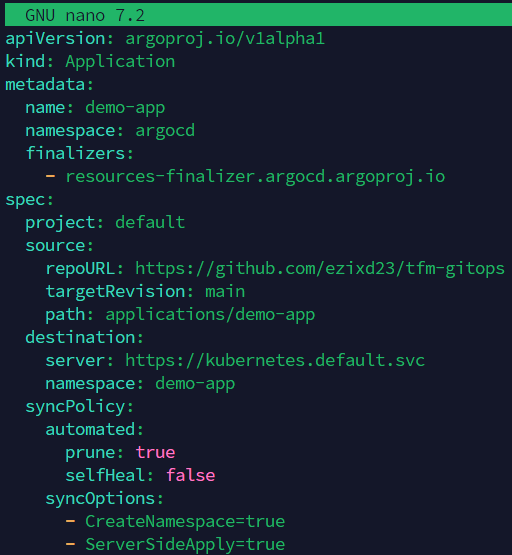
\includegraphics[width=0.70\linewidth]{actions/bloque5_app-demo.png}
\caption{Manifest \texttt{app-demo.yaml}: Application for the workload with \texttt{selfHeal:\,false}}
\label{fig:app-demo-yaml}
\end{figure}

This decision reflects an important operational distinction between the two managed planes. Security policies are platform assets whose integrity is critical: any deviation from their declarative state in Git constitutes a potential security posture degradation and must be automatically reverted. Workload resources, on the other hand, may be temporarily modified by the operations team for diagnostics, by auto-scaling scripts or by other cluster controllers without representing a security problem. The \texttt{selfHeal:\,false} delegates to the team the decision of when to reconcile, maintaining declarative control (Git as source of truth) but without the automatic reversal that can interfere with legitimate operations.

After applying the manifest, ArgoCD detects the divergence between the repository and the cluster (which does not yet contain any resources from the \texttt{demo-app} namespace) and proceeds with synchronisation. Figure~\ref{fig:demo-argocd} shows the resulting resource tree: the \texttt{Application} \texttt{demo-app} manages the Namespace, Service and Deployment, which in turn generates a ReplicaSet with two active Pods.

\begin{figure}[H]
\centering
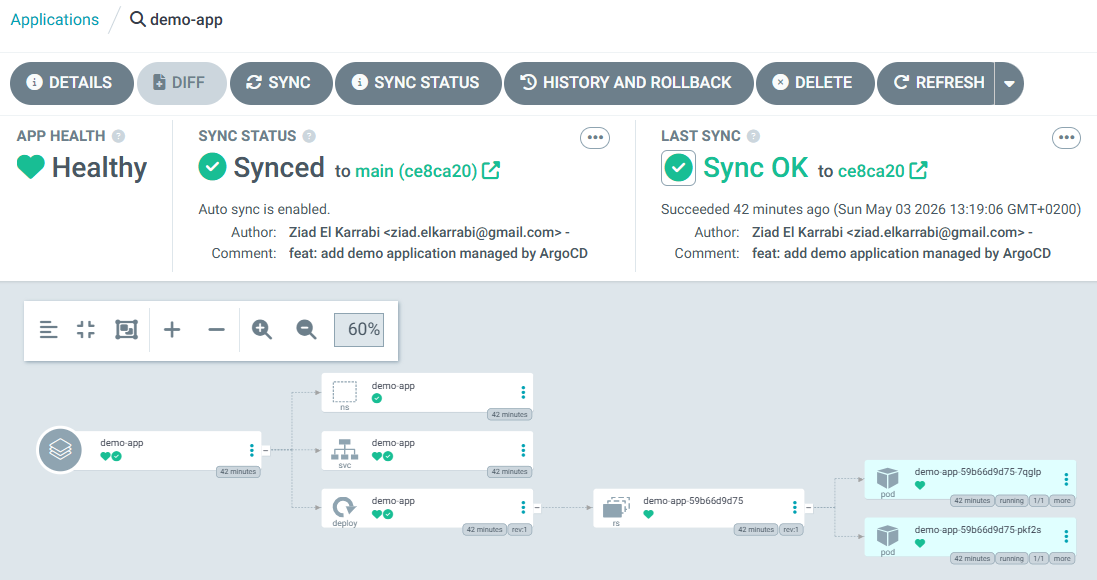
\includegraphics[width=0.95\linewidth]{actions/bloque5_argocd-demo-app.png}
\caption{Resource tree of the \texttt{demo-app} Application: Namespace, Service, Deployment and two Pods}
\label{fig:demo-argocd}
\end{figure}

\subsection{Verification of Kyverno mutations}

Figure~\ref{fig:demo-outputs} shows the integrated verification of the effects of mutation policies on the demo application pods.

\begin{figure}[H]
\centering
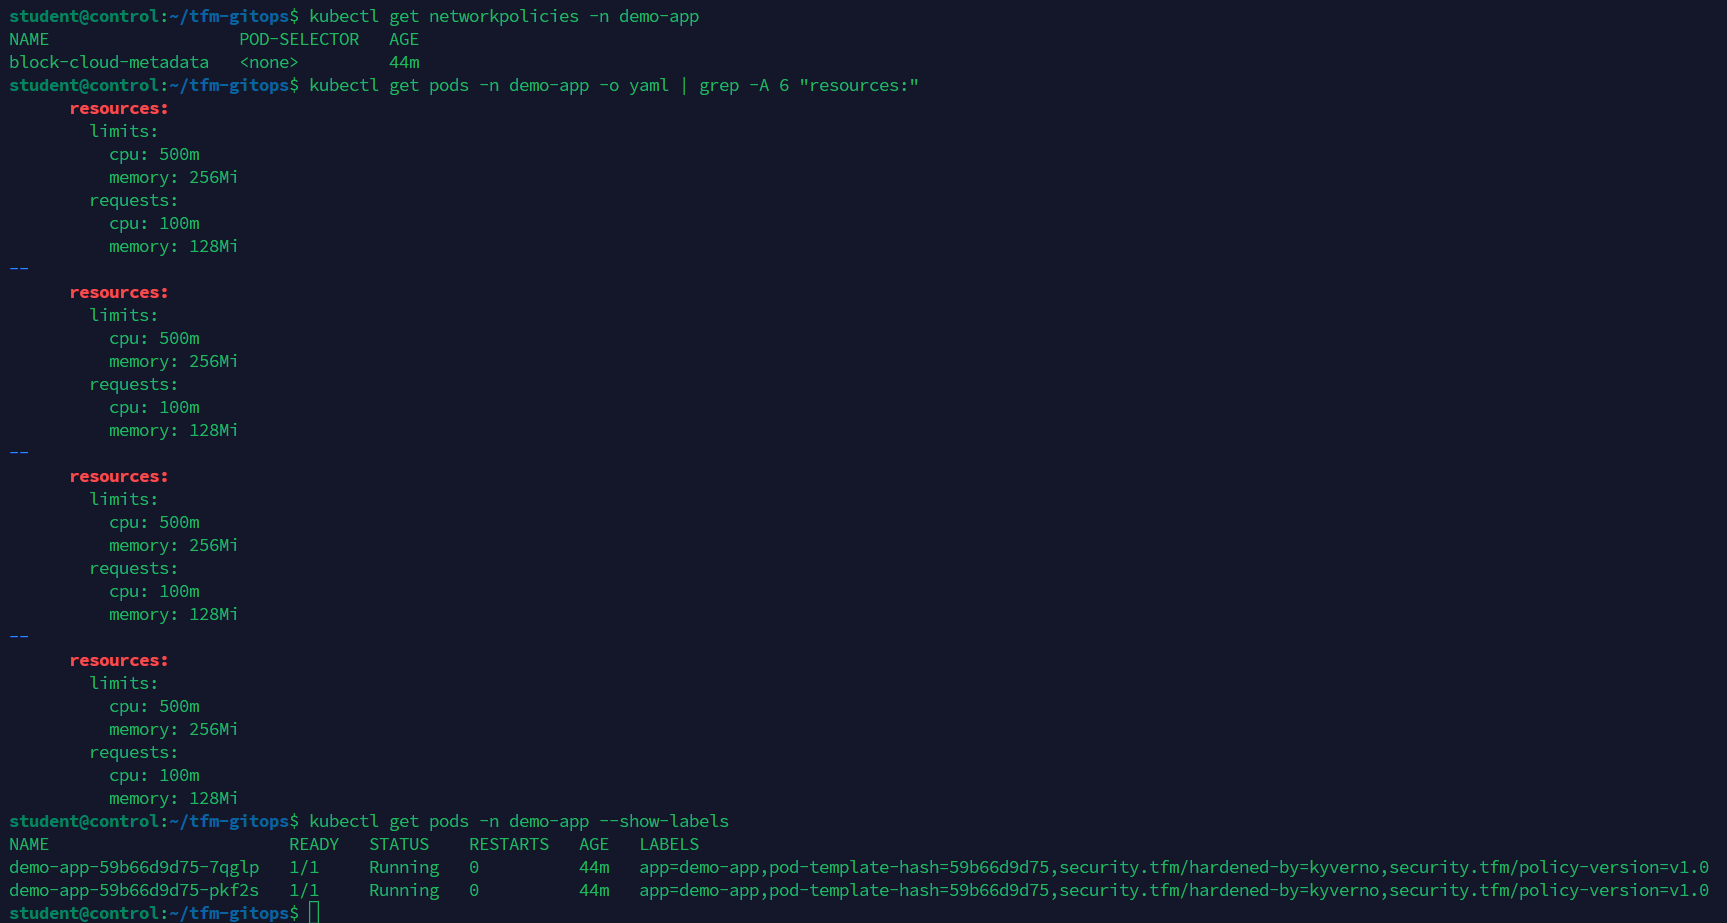
\includegraphics[width=0.95\linewidth]{actions/bloque5_ouputsP4P7P8.png}
\caption{Verification of mutations P4, P7 and P8 on the demo application pods}
\label{fig:demo-outputs}
\end{figure}

The query \texttt{kubectl get networkpolicies -n demo-app} confirms that the NetworkPolicy \texttt{block-cloud-metadata} has been automatically generated by P8 in the \texttt{demo-app} namespace at the moment of its creation, without any manual intervention. The NetworkPolicy has existed for 44~minutes, an identical period to the rest of the namespace resources, confirming that generation occurred immediately.

The query of the following command:

\begin{lstlisting}
kubectl get pods -n demo-app -o yaml | grep -A 6 "resources:"
\end{lstlisting}

shows that all containers in the ReplicaSet pods have injected \texttt{limits} (cpu:\,500m, memory:\,256Mi) and \texttt{requests} (cpu:\,100m, memory:\,128Mi) fields by policy P4, despite the Deployment declared in Git specifying no \texttt{resources} field. The count of four \texttt{resources} blocks is due to the \texttt{grep} command capturing all occurrences of the \texttt{resources:} pattern in the pod's YAML manifest ---both in \texttt{spec.containers} (the desired specification) and in \texttt{status.containerStatuses} (the actual state reported by the kubelet)---, repeated for the two active pods in the ReplicaSet.

The query \texttt{kubectl get pods -n demo-app -{}-show-labels} confirms the presence of the labels \texttt{security.tfm/\allowbreak hardened-by:\,\allowbreak kyverno} and \texttt{security.tfm/\allowbreak policy-version:\,\allowbreak v1.0} injected by P7 on both pods, alongside the Deployment's own labels (\texttt{app:\,\allowbreak demo-app}, \texttt{pod-template-hash}).
The HTTP verification, shown in Figure~\ref{fig:nginx-ok}, confirms that the application is functionally correct despite the complete set of applied security restrictions: nginx responds correctly at \texttt{192.168.1.101:8888}.

\begin{figure}[H]
\centering
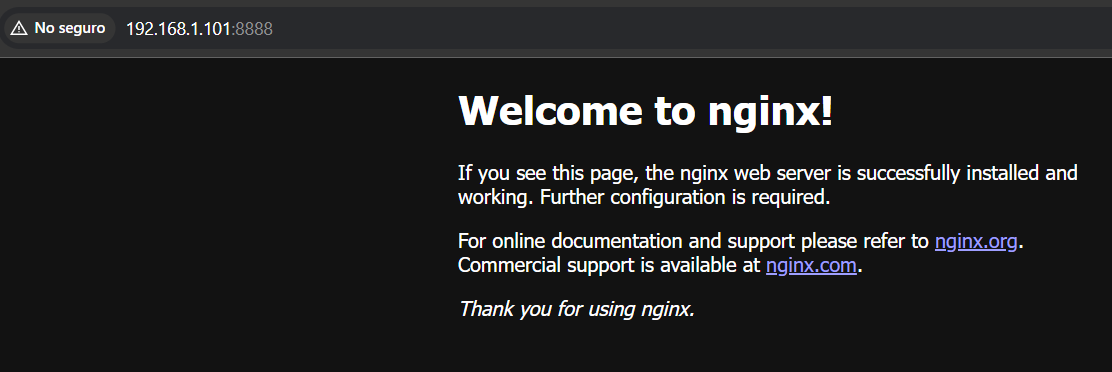
\includegraphics[width=0.85\linewidth]{actions/bloque5_outputNgnixFuncionando.png}
\caption{Demo application accessible and functional at \texttt{192.168.1.101:8888} with all policies active}
\label{fig:nginx-ok}
\end{figure}

Figure~\ref{fig:dos-applications} shows the final ArgoCD panel state with both \texttt{Application} objects ---\texttt{demo-app} and \texttt{kyverno-policies}--- both in \texttt{Healthy}~+~\texttt{Synced} state, materialising the two-plane GitOps architecture described in Chapter~5.

\begin{figure}[H]
\centering
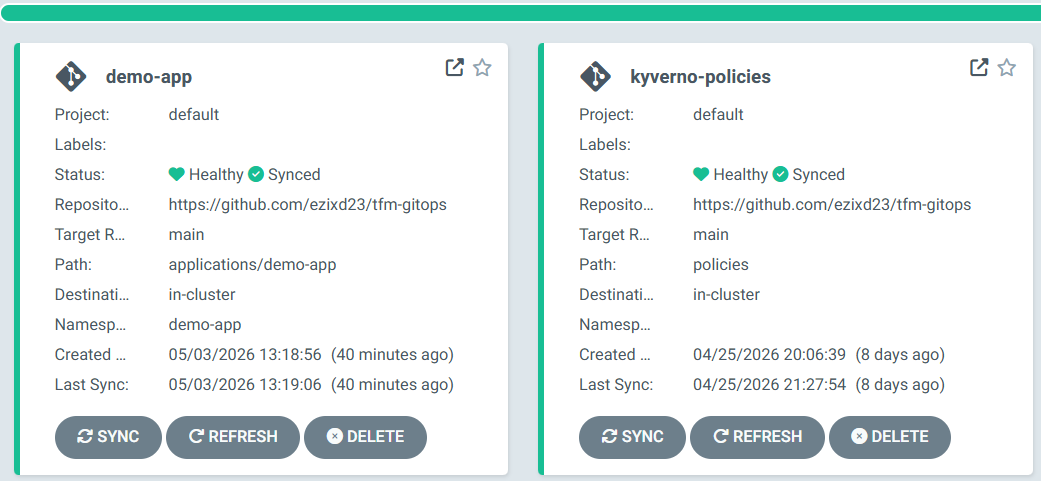
\includegraphics[width=0.85\linewidth]{actions/bloque5_dosAplications.png}
\caption{Final ArgoCD panel state: two Applications in Healthy and Synced state}
\label{fig:dos-applications}
\end{figure}

% ─────────────────────────────────────────────
\section{Analysis: interaction between mutating webhooks and ArgoCD}
\label{sec:argocd-mutating}
% ─────────────────────────────────────────────

ArgoCD's official documentation explicitly warns that the presence of \textit{mutating admission controllers} in the cluster can generate permanent \textit{drift} \cite{argocd_diffing}: if a webhook modifies a resource after ArgoCD has synchronised it, the state in the cluster will differ from the state in Git indefinitely, chronically maintaining the \texttt{Application} in \texttt{OutOfSync} state. The prescribed solution is the \texttt{ignoreDifferences} or \texttt{ServerSideApply} options. Section~\ref{sec:ignore-differences} already documented the application of this solution for the case of defaults injected by Kyverno on the \texttt{ClusterPolicies} themselves. This section analyses whether the same problem manifests for the mutations Kyverno applies to the demo application pods.

\subsection{Observed behaviour: absence of drift in the demo Application}

The \texttt{Application} \texttt{demo-app} remains stably in \texttt{Synced}~+~\texttt{Healthy} state, as confirmed by Figure~\ref{fig:escenario1-sync}, despite its pods being mutated by the four policies P4--P7. This result, which might seem counterintuitive given the documentation warning, has a precise technical explanation.

\begin{figure}[H]
\centering
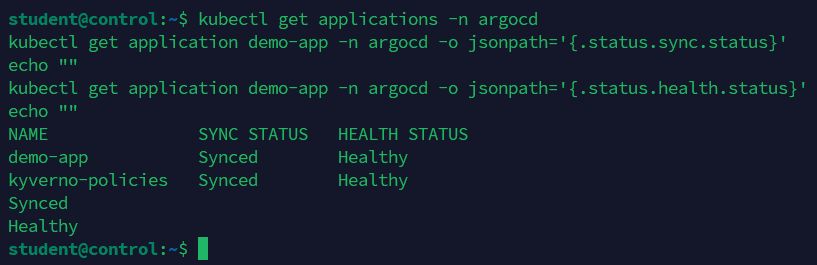
\includegraphics[width=0.85\linewidth]{actions/bloque5_escenario1Sync.png}
\caption{Both Applications in Synced and Healthy state: pod mutation does not generate drift in ArgoCD}
\label{fig:escenario1-sync}
\end{figure}

ArgoCD compares resources at the same hierarchical level at which they are declared in Git. The repository contains a resource of type \texttt{Deployment}, not \texttt{Pod} resources directly. Kyverno's mutations ---P4 (resources), P5 (securityContext), P6 (readOnlyRootFilesystem) and P7 (labels)--- are applied to the \texttt{Pod} at the time of its creation by the ReplicaSet, not to the \texttt{spec.template} field of the \texttt{Deployment}. ArgoCD compares the \texttt{Deployment} declared in Git with the \texttt{Deployment} existing in the cluster, and these match. The \texttt{Pod} resources generated as child resources are not directly managed by ArgoCD and do not form part of the comparison.

The empirical verification of this behaviour, documented in Figure~\ref{fig:escenario1-mutacion}, compares the content of the \texttt{Deployment} and a \texttt{Pod} in the cluster by searching for relevant fields:

\begin{figure}[H]
\centering
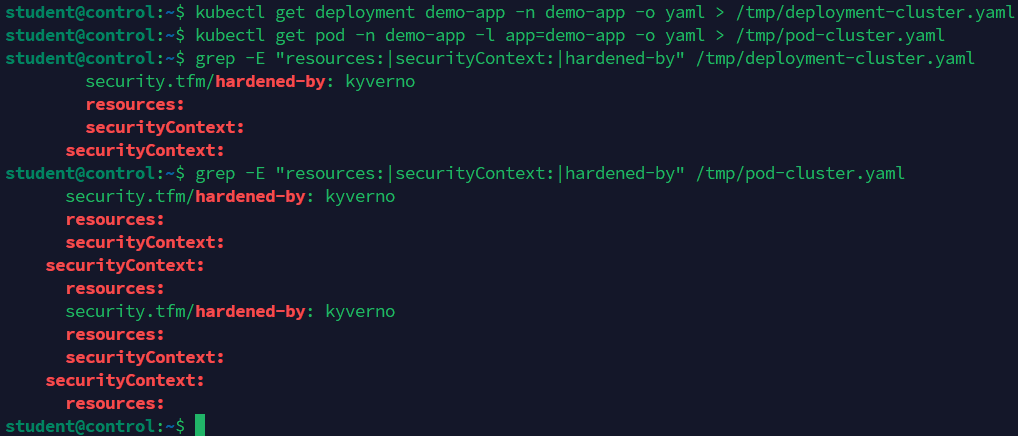
\includegraphics[width=0.95\linewidth]{actions/bloque5_escenario1Mutacion.png}
\caption{Deployment vs. Pod comparison: mutations exist in the Pod but not in the \texttt{spec.template} of the Deployment}
\label{fig:escenario1-mutacion}
\end{figure}

The search on \texttt{/tmp/deployment-cluster.yaml} returns \texttt{resources:} with empty value (the field exists in the object but without assigned values in the template) and \texttt{securityContext:} only with \texttt{runAsNonRoot:\,true} and \texttt{runAsUser:\,101}, which correspond to the values explicitly declared in the Git manifest. The search on \texttt{/tmp/pod-cluster.yaml} returns \texttt{resources:} with values injected by P4 (\texttt{limits} and \texttt{requests}), multiple \texttt{securityContext:} entries with values injected by P5 and P6, and the presence of the label \texttt{security.tfm/hardened-by:\,kyverno} injected by P7. The injected fields exist in the Pod but not in the Deployment, and ArgoCD only compares Deployments.

This observation is related to the autogen mechanism described in Section~\ref{subsec:autogen}. The rules \texttt{autogen-add-resources}, \texttt{autogen-add-default-securitycontext} and similar, visible in Figure~\ref{fig:autogen-deployment}, generate additional rules that apply to the \texttt{spec.template.spec} of higher-level controllers, not only to the resulting Pods.

\begin{figure}[H]
\centering
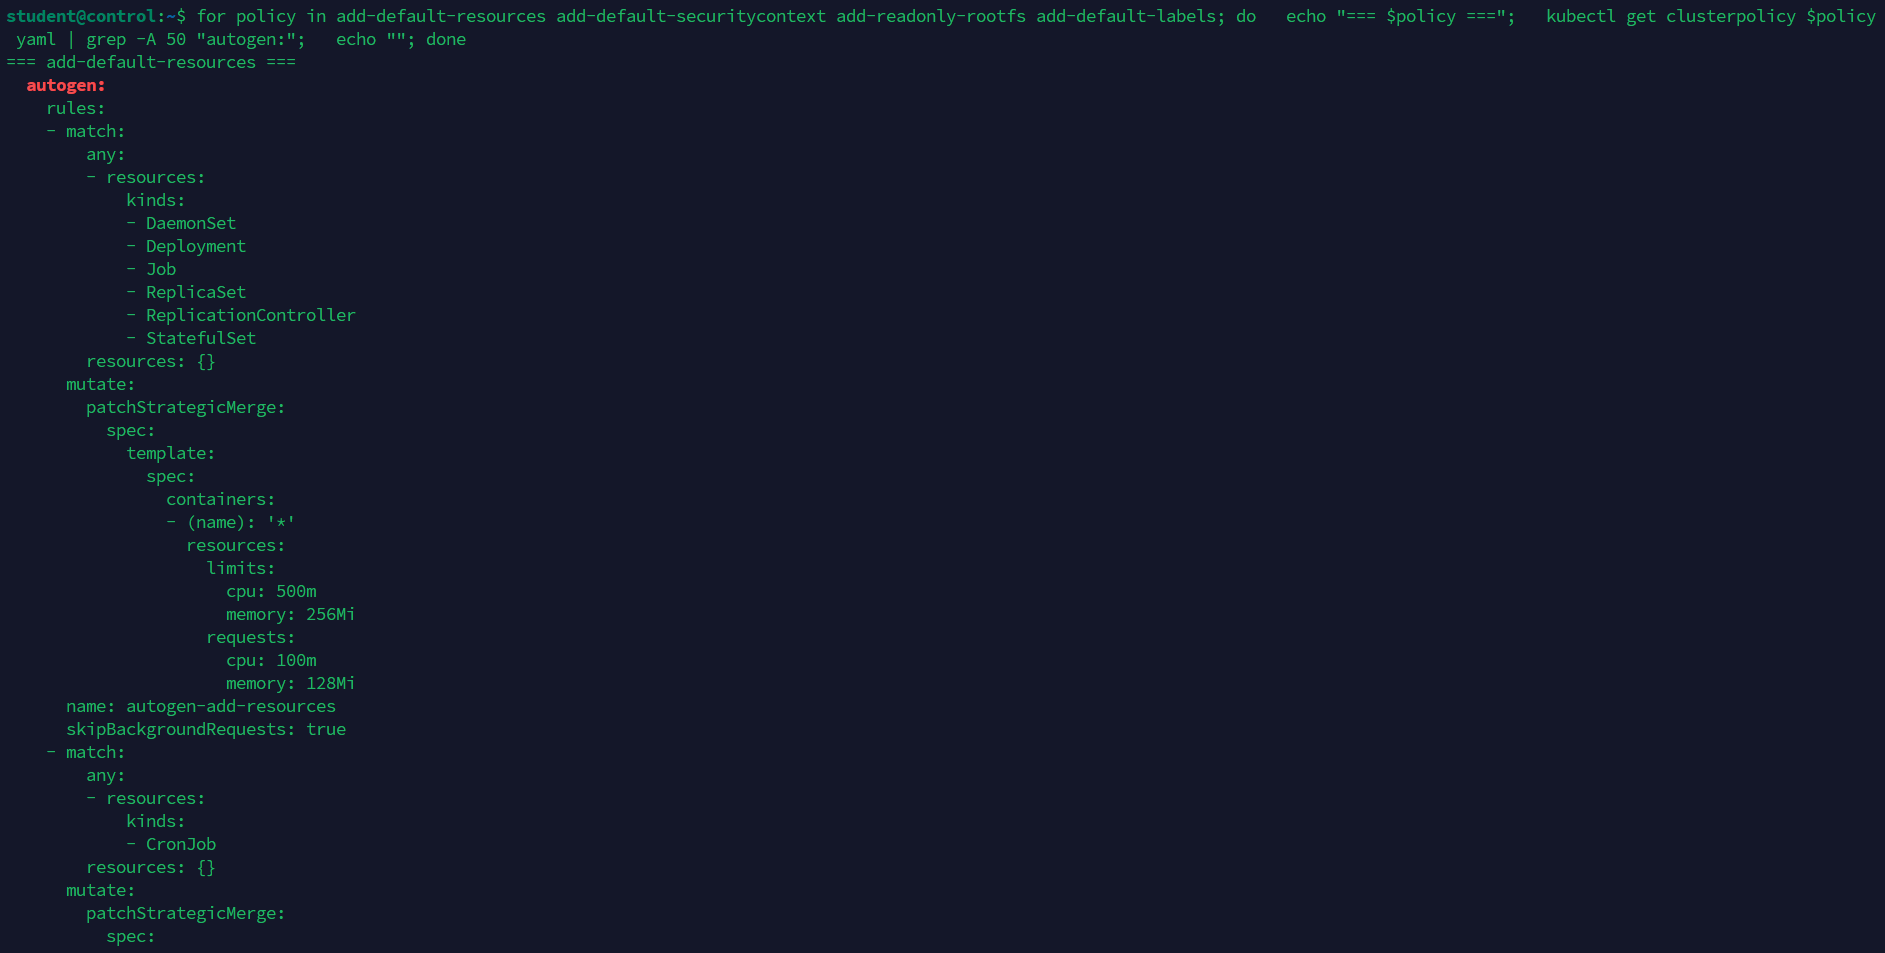
\includegraphics[width=0.95\linewidth]{actions/bloque5_escenario1Autogen.png}
\caption{Autogen rules for policy P4: cover Deployment, StatefulSet, Job, ReplicaSet via \texttt{spec.template.spec}}
\label{fig:autogen-deployment}
\end{figure}

However, empirical comparison demonstrates that the \texttt{spec.template} of the Deployment in the cluster does not contain the injected fields. This indicates that in the version of Kyverno used (v1.13) with \texttt{patchStrategicMerge}, the effective mutation occurs only on the \texttt{Pod} object at the time of its creation by the ReplicaSet, not on the \texttt{spec.template} of the Deployment at admission time. This behaviour is consistent with the principle of minimum interference with external declarative systems such as ArgoCD.

\subsection{Verification of the case where drift does occur}

To confirm that the described mechanism is correct and not simply an absence of mutation, an experimental policy ---\texttt{experimental-\allowbreak deployment-\allowbreak labels}--- is designed that explicitly mutates \texttt{Deployment} type resources by adding a label \texttt{experimental.tfm/\allowbreak deployment-mutated:\,\allowbreak "true"} directly to the \texttt{Deployment} object, as shown in Figure~\ref{fig:policy-experimental}.
\begin{figure}[H]
\centering
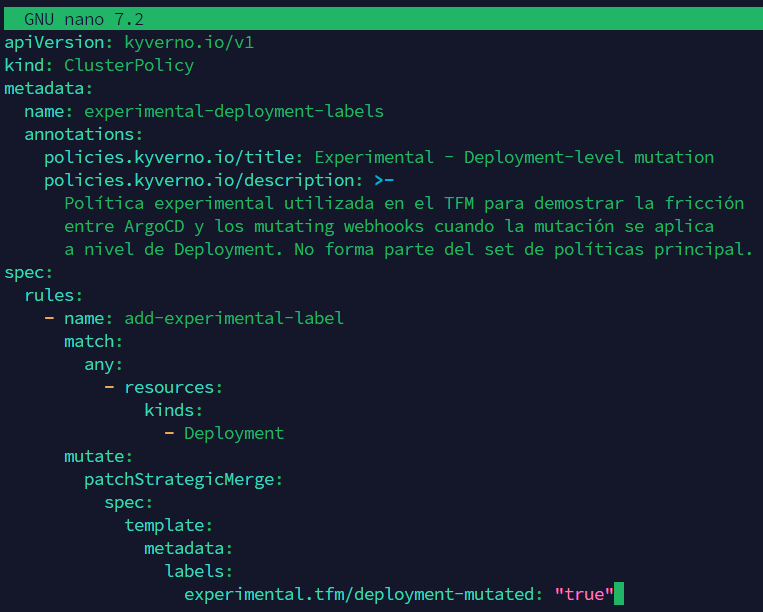
\includegraphics[width=0.72\linewidth]{actions/bloque5_escenario2policy-experimental-deployment-labels.png}
\caption{Experimental policy that directly mutates \texttt{Deployment} type resources}
\label{fig:policy-experimental}
\end{figure}
\vspace{-\parskip}

Figure~\ref{fig:escenario2-outsync} shows the result: immediately after applying this policy in the cluster, the \texttt{Application} \texttt{demo-app} transitions to \texttt{OutOfSync} state while \texttt{kyverno-policies} remains \texttt{Synced}. The \texttt{Deployment} in the cluster now has the additional label not declared in Git, and ArgoCD correctly detects the divergence.

\begin{figure}[H]
\centering
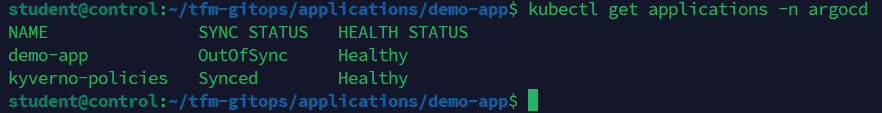
\includegraphics[width=0.85\linewidth]{actions/bloque5_escenario2OutputdelComandoKubectl.png}
\caption{Real drift case test: \texttt{demo-app} transitions to OutOfSync when directly mutating the Deployment}
\label{fig:escenario2-outsync}
\end{figure}

This experiment simultaneously confirms two things: first, that ArgoCD's drift detection mechanism works correctly when mutation affects the level of the managed resource; second, that the main set's mutation policies (P4--P7) do not produce this effect because they operate at Pod level and not at Deployment level, which constitutes the correct design for their coexistence with GitOps systems.

\subsection{Conclusion and resolution pattern}

Empirical analysis allows formulating a precise technical conclusion: in the implemented setup, the friction between Kyverno's \textit{mutating webhooks} and ArgoCD does not manifest for the main set's mutation policies because these operate at a different hierarchical level than the resources managed by ArgoCD. The official documentation warning is correct in general, but not applicable to this specific design.

In scenarios where policies directly mutated resources of the same type as those managed in Git ---for example, \texttt{spec.replicas} mutations in Deployments or addition of labels at the Deployment level--- it would be necessary to configure \texttt{ignoreDifferences} in the corresponding \texttt{Application} for the affected fields. The resolution pattern already documented in Section~\ref{sec:ignore-differences} ---use of \texttt{jqPathExpressions} to exclude fields modified by the system--- is directly applicable to this case, without requiring changes to the Git manifests or Kyverno policies.

\chapter{Continuous Integration with GitHub Actions and Vulnerability Analysis}

This chapter documents the implementation of the Continuous Integration layer of the DevSecOps environment, completing the architecture designed in Chapter~5 and closing the CI/CD cycle begun with ArgoCD in Chapter~7. Up to this point, the GitOps architecture operated with a single repository (\texttt{tfm-gitops}) combining Kubernetes manifests and security policies, managed declaratively by ArgoCD. This chapter materialises the \textit{two-repository pattern} announced in Section~7.1: a second repository (\texttt{tfm-demo-app}) is introduced, containing the application source code and its Dockerfile, and the Continuous Integration pipeline is implemented to build the image, subject it to security analysis, and propagate the change to the GitOps repository for automatic deployment.

A central technical feature of the pipeline is the adoption of a \textit{defence in depth} strategy for vulnerability analysis: instead of a single scanning engine, two complementary engines are implemented. Trivy \cite{trivy_docs} analyses the locally built image, and Grype \cite{grype_docs} analyses an SBOM (\textit{Software Bill of Materials}) \cite{syft_docs} generated by Syft from that same image, consulting different CVE databases. The empirical finding that justifies this strategy---Trivy passed the \texttt{python:3.12-slim} image without alerts while Grype detected a HIGH-severity vulnerability that blocked the pipeline---is one of the most relevant results of this work.

The chapter is organised into seven sections. The first justifies the two-repository split and documents its structure. The second describes the image registry configuration and pipeline credentials. The third documents the demo application and its Dockerfiles. The fourth describes the design of the GitHub Actions workflow and its security decisions. The fifth analyses in depth the dual-engine scanning strategy and the key empirical finding. The sixth covers the technical incidents and lessons learned during implementation. The seventh documents the closure of the complete CI/CD cycle and the integration with the GitOps repository.

% ─────────────────────────────────────────────
\section{Application repository design and two-repository strategy}
% ─────────────────────────────────────────────

The separation between the application repository and the configuration repository is not an organisational preference, but a concrete security requirement justified in Section~5.5.1. The central principle is credential segregation: the CI pipeline needs access to the image registry (\texttt{quay.io}) and write access to the configuration repository, but must under no circumstances have direct access to the Kubernetes cluster. ArgoCD, in turn, needs access to the configuration repository to synchronise the cluster state, but has no reason to access the application source code. This separation establishes a security perimeter between the two phases of the CI/CD cycle, so that the compromise of one does not automatically imply the compromise of the other.

The \texttt{tfm-demo-app} repository contains exclusively the application-layer artefacts:

\begin{itemize}
  \item \texttt{app/}: Python Flask application source code, including the main module (\texttt{app.py}) and the dependency file (\texttt{requirements.txt}).
  \item \texttt{docker/}: the two project Dockerfiles (\texttt{Dockerfile} and \texttt{Dockerfilevulnerable}).
  \item \texttt{.github/workflows/}: the GitHub Actions workflow (\texttt{build-and-push.yaml}) implementing the complete CI pipeline.
\end{itemize}

The \texttt{tfm-gitops} repository, managed by ArgoCD since Chapter~7, is not modified by the development team: only the CI pipeline updates it, and only the \texttt{image} field of the demo application manifest. This delimitation ensures that the security policy manifests (directory \texttt{policies/}) and the ArgoCD \texttt{Application} configuration remain under strict, separate control from the application development cycle.

This architecture materialises the flow described in Section~5.3.1: a commit to the application repository triggers the CI pipeline, which culminates with a commit to the configuration repository, which in turn acts as the trigger signal for ArgoCD. The cluster never receives direct instructions from the pipeline: all interaction with Kubernetes is mediated by the GitOps repository and the reconciliation controller.

% ─────────────────────────────────────────────
\section{Image registry configuration and credentials}
% ─────────────────────────────────────────────

The chosen image registry is Quay.io \cite{quay_docs}, in line with the tools presented in the course and as an enterprise-grade alternative to Docker Hub. Pipeline authentication against the registry is performed via a \textbf{Robot Account}, a central concept in credential management for CI/CD systems that warrants explicit technical justification.

A Robot Account is a non-personal service account whose credentials are decoupled from any individual user. In a CI/CD pipeline, using personal credentials presents two security problems: the first is the \textit{blast radius} in case of compromise---personal credentials have access to all repositories of the user---; the second is operational continuity---if the user leaves the organisation, the pipeline stops working---. A Robot Account addresses both problems: it has access exclusively to the repositories explicitly assigned to it, with the minimum permission level required for its function.

The Robot Account created is named \texttt{zelkarrabi+tfm\_ci\_robot}. Figure~\ref{fig:ci-robotaccount} shows its permission configuration in Quay.io: it has \textit{Write} permission on the \texttt{tfm-demo-app} repository and \textit{None} permission on the \texttt{prova} repository, which is an unrelated test repository. This granularity confirms the application of the least-privilege principle: the Robot Account can only publish images in the specific repository for which it was created, and cannot modify its configuration or access other repositories.

\begin{figure}[H]
\centering
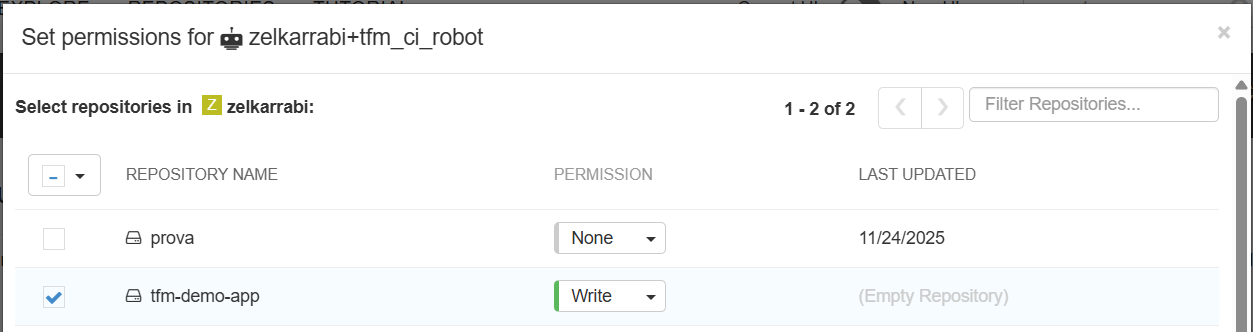
\includegraphics[width=0.90\linewidth]{ci_cd/bloque1_robotaccount.png}
\caption{Configuration of the Robot Account \texttt{zelkarrabi+tfm\_ci\_robot} in Quay.io: \textit{Write} permission on \texttt{tfm-demo-app} and no access on other repositories}
\label{fig:ci-robotaccount}
\end{figure}

The Robot Account credentials are validated beforehand using \texttt{podman login quay.io} from the cluster control node, confirming that the credentials are functional before configuring them in the pipeline. Figure~\ref{fig:ci-podmanlogin} shows the successful authentication with user \texttt{zelkarrabi}.

\begin{figure}[H]
\centering
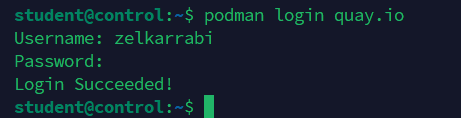
\includegraphics[width=0.60\linewidth]{ci_cd/bloque1_podmanLogin.png}
\caption{Registry credential verification: successful authentication at \texttt{quay.io} via \texttt{podman login}}
\label{fig:ci-podmanlogin}
\end{figure}
\vspace{-\parskip}

The pipeline requires three repository secrets in GitHub, whose configuration is shown in Figure~\ref{fig:ci-secrets}:

\begin{figure}[H]
\centering
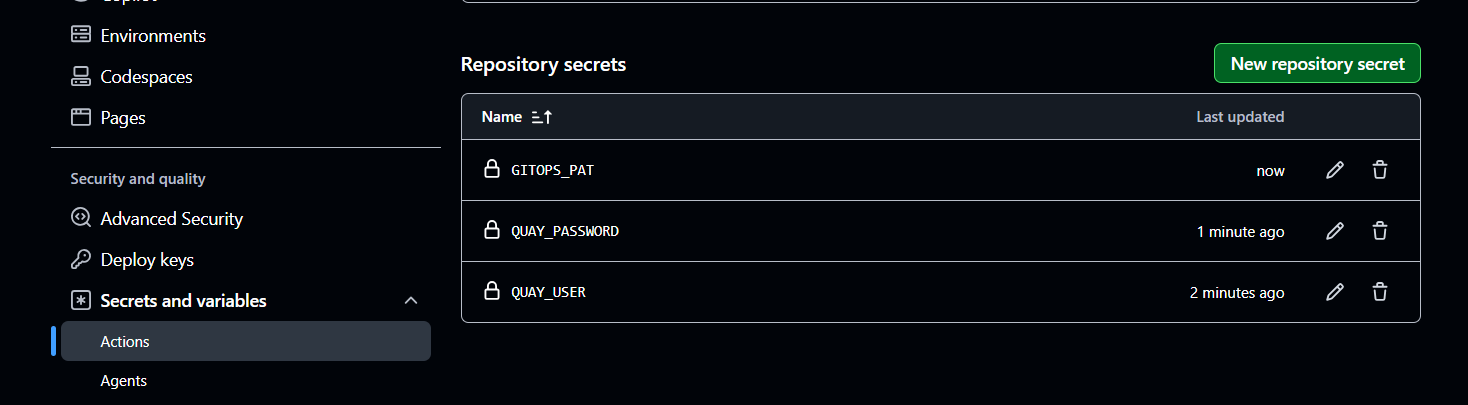
\includegraphics[width=0.90\linewidth]{ci_cd/bloque2_creaccionSecrets.png}
\caption{The three repository secrets configured in GitHub Actions: \texttt{GITOPS\_PAT}, \texttt{QUAY\_PASSWORD} and \texttt{QUAY\_USER}}
\label{fig:ci-secrets}
\end{figure}

\begin{itemize}
  \item \texttt{QUAY\_USER}: Robot Account name (\texttt{zelkarrabi+tfm\_ci\_robot}) for authentication at Quay.io.
  \item \texttt{QUAY\_PASSWORD}: access token generated by Quay.io for the Robot Account.
  \item \texttt{GITOPS\_PAT}: GitHub Personal Access Token for cross-repository writes to \texttt{tfm-gitops}. Unlike the Quay.io Robot Account, a classic PAT with \texttt{repo} scope does not apply the least-privilege principle: it grants read and write access to \textit{all} the user's repositories, not only \texttt{tfm-gitops}. The correct alternative is a \textit{fine-grained PAT} explicitly limited to \texttt{tfm-gitops} with \texttt{Contents: read/write} permission, which replicates for GitHub the same granularity the Robot Account offers in Quay.io; a \textit{deploy key} is another equivalent option. In this lab environment a classic PAT is used for simplicity, with the awareness that in production it should be replaced with one of those alternatives.
\end{itemize}

The explicit use of \texttt{GITOPS\_PAT} instead of the default \texttt{GITHUB\_TOKEN} is a technical constraint of GitHub Actions: the \texttt{GITHUB\_TOKEN} has permissions only over the repository in which the workflow runs (\texttt{tfm-demo-app}), and cannot write to a different repository. The \texttt{GITOPS\_PAT}, being a personal token with explicit scope over \texttt{tfm-gitops}, is the correct mechanism for cross-repository writes.

% ─────────────────────────────────────────────
\section{The demo application and the Dockerfiles}
% ─────────────────────────────────────────────

The demo application is a minimal Python Flask application whose purpose is to validate the complete CI/CD cycle, not to represent a real production workload. It exposes two endpoints on port~8080:

\begin{lstlisting}
from flask import Flask, jsonify
import os, socket

app = Flask(__name__)

@app.route('/')
def index():
    return jsonify({
        "service": "tfm-demo-app",
        "version": "1.0.0",
        "status": "ok",
        "hostname": socket.gethostname(),
        "ci_pipeline": os.getenv("CI_PIPELINE", "manual")
    })

@app.route('/health')
def health():
    return jsonify({"status": "healthy"})

if __name__ == '__main__':
    app.run(host='0.0.0.0', port=8080)
\end{lstlisting}

The root endpoint (\texttt{/}) returns a JSON object that includes the service name, version, pod hostname, and the value of the \texttt{CI\_PIPELINE} environment variable. This last field is what makes it possible to verify empirically, at the end of the chapter, that the code deployed in the cluster corresponds exactly to the commit that triggered the pipeline. The \texttt{/health} endpoint serves as a readiness probe for Kubernetes components.

\subsection{The secure Dockerfile: technical decisions}

The main Dockerfile incorporates several security-oriented design decisions that merit explicit justification:

\begin{lstlisting}
# Stage 1: builder
FROM python:3.13-slim AS builder
WORKDIR /build
COPY app/requirements.txt .
RUN pip install --no-cache-dir --user --upgrade pip && \
    pip install --no-cache-dir --user -r requirements.txt

# Stage 2: runtime
FROM python:3.13-slim
RUN groupadd -r -g 10001 appuser && \
    useradd -r -u 10001 -g appuser appuser

WORKDIR /app
COPY --from=builder --chown=appuser:appuser /root/.local /home/appuser/.local
COPY --chown=appuser:appuser app/app.py /app/

ENV PATH="/home/appuser/.local/bin:${PATH}" \
    PYTHONUNBUFFERED=1 \
    PYTHONDONTWRITEBYTECODE=1

USER appuser
EXPOSE 8080
CMD ["python", "/app/app.py"]
\end{lstlisting}

\textbf{Multi-stage build.} The separation between the \texttt{builder} stage and the runtime stage is the highest-impact decision on the attack surface of the image. The \texttt{builder} stage installs dependencies with \texttt{pip install --user}, which places them in \texttt{/root/.local}. The runtime image copies only that directory---with \texttt{--chown=appuser:appuser}---to the \texttt{/home/appuser/.local} directory of the application user. This way, the \texttt{pip} binary and its own transitive dependencies are not present in the final artefact, reducing the number of scannable components and the exploitation surface at runtime.

\textbf{Minimal base image (\texttt{python:3.13-slim}).} The \texttt{slim} variant of the official Python image removes non-essential operating system packages included in the standard image. This choice represents a balance between compatibility and security: the image includes the system libraries required by most Python applications, but removes development tools, scripting interpreters, and utilities that could be leveraged after an intrusion. The extreme of this strategy is Google's \textit{distroless} \cite{distroless_docs} images, which remove even the shell and package manager, reducing the attack surface to the absolute minimum at the cost of some complexity in runtime failure diagnostics.

\textbf{Non-root user with UID~10001.} The Dockerfile creates \texttt{appuser} as a system account (\texttt{groupadd -r}, \texttt{useradd -r}): without a login shell, without an entry in \texttt{/etc/passwd} with an explicit home, with UID~10001 that avoids collisions with system UIDs (0--999) and typical user UIDs (1000+). The \texttt{USER appuser} instruction makes that identity effective for all container processes. This constitutes a defence-in-depth layer consistent with policy P1 (\texttt{disallow-root}) from Chapter~6: although Kyverno would reject any pod without \texttt{runAsNonRoot:\,true}, the defence starts earlier, in the Dockerfile itself, so that the image operates with minimum privilege regardless of the cluster in which it is deployed.

\textbf{Python environment variables.} \texttt{PYTHONUNBUFFERED=1} ensures that the process standard output is not buffered, allowing logs to be captured in real time by the Kubernetes logging system. \texttt{PYTHONDONTWRITEBYTECODE=1} prevents the writing of \texttt{.pyc} files to the container filesystem, which is consistent with policy P6 (\texttt{add-readonly-rootfs}) that forces the root filesystem to read-only mode: without this variable, Python would attempt to write compiled bytecode and generate permission errors at runtime.

\textbf{Flag \texttt{-{}-no-cache-dir}.} Installing dependencies with this option prevents pip from caching downloaded packages inside the image, reducing its final size and eliminating unnecessary content that might contain outdated package versions.

\subsection{The vulnerable Dockerfile as a reference artefact}

The repository includes a second Dockerfile, \texttt{Dockerfilevulnerable}, based on \texttt{python:3.4-alpine}. Python~3.4 reached end of life in March 2019 and accumulates hundreds of documented CVEs with no fix available in that branch. This artefact was originally designed as a controlled test mechanism to demonstrate the pipeline blocking scenario when facing images with critical vulnerabilities. However, as documented in Section~8.6, this artificial scenario proved unnecessary: the development cycle itself organically produced a genuine block that constitutes empirical evidence of greater academic value than any artificial test.

% ─────────────────────────────────────────────
\section{Continuous Integration pipeline design}
\label{sec:pipeline-design}
% ─────────────────────────────────────────────

The pipeline is defined in the file \texttt{.github/workflows/build-and-push.yaml}. The workflow name is \textit{Build, Scan and Push to Quay} and its single job is named \textit{Build, Trivy scan and push}. The trigger is \texttt{push} on the \texttt{main} branch with path filters that restrict execution to commits affecting the \texttt{app/} directory, the \texttt{docker/} directory, or the workflow file itself:

\begin{lstlisting}
on:
  push:
    branches: [main]
    paths:
      - 'app/**'
      - 'docker/**'
      - '.github/workflows/**'
\end{lstlisting}

This configuration prevents commits affecting only documentation or auxiliary files from unnecessarily triggering the pipeline, reducing GitHub Actions minute consumption and noise in the execution history.

\subsection{Pipeline security decisions}

The four pipeline security design decisions merit explicit technical justification, as they directly materialise the principles stated in Chapter~5.

\textbf{Version pinning via SHA hash.} All third-party GitHub Actions used in the pipeline are referenced by their full commit SHA hash, rather than by semantic version tags or floating tags such as \texttt{@v4} or \texttt{@latest}. For example:

\begin{lstlisting}
- uses: actions/checkout@b4ffde65f46336ab88eb53be808477a3936bae11  # v4.1.1
\end{lstlisting}

This practice materialises the defence against the attack vector documented in Section~5.5.6: a tag like \texttt{@v4} can be redirected by the action maintainer (or by an attacker who has compromised their account) to a different commit without the reference name changing. A SHA hash, by contrast, is immutable: if the workflow manifest references SHA \texttt{b4ffde65f46\ldots}, the runner will execute exactly that commit, regardless of what happens to the repository tags. The limitation of this mechanism, documented as an incident in Section~8.6, is that it does not protect against transitive dependencies of the action code itself.

\textbf{Minimum runner permissions.} The job permission block explicitly declares only the necessary permissions:

\begin{lstlisting}
permissions:
  contents: read
\end{lstlisting}

The default \texttt{GITHUB\_TOKEN} in GitHub Actions has write permissions over the repository. This explicit declaration of \texttt{contents: read} revokes those default permissions, so that even if the runner environment were compromised during execution, the exfiltrated token could not modify the application repository.

\textbf{Image tag based on the commit short SHA.} The tag of the image published in Quay.io is computed from the short SHA of the commit that triggered the pipeline:

\begin{lstlisting}
- name: Compute image tag
  id: vars
  run: |
    SHORT_SHA=$(echo "${GITHUB_SHA}" | cut -c1-7)
    echo "SHORT_SHA=${SHORT_SHA}" >> $GITHUB_OUTPUT
    echo "FULL_IMAGE=${REGISTRY}/${IMAGE_NAME}:${SHORT_SHA}" >> $GITHUB_OUTPUT
\end{lstlisting}

This decision implements the supply chain traceability and immutability principle: each image published in the registry corresponds bijectively to a specific commit in the application repository, making it possible to audit at any time exactly which code is running in the cluster. This design is also consistent with policy P9 (\texttt{disallow-latest-tag}) introduced in Section~7.5.2, which rejects pods whose images are tagged with \texttt{:latest}: the pipeline never produces floating tags, only commit-SHA-based tags.

\textbf{Separation of build and push.} The image is built locally on the runner without being published (\texttt{push: false}). Vulnerability scanning runs against the locally built image. Only if all security controls pass their thresholds is the publication step executed. This sequence implements the \textit{fail fast} principle: a vulnerable image never reaches the registry, eliminating the risk of ArgoCD detecting and deploying it before the incident is identified and managed.

\subsection{Complete pipeline step sequence}

Figure~\ref{fig:ci-workflow-steps-final} shows the step view of the complete workflow in its final version, with the 15 steps that form the pipeline in a successful state:

\begin{figure}[H]
\centering
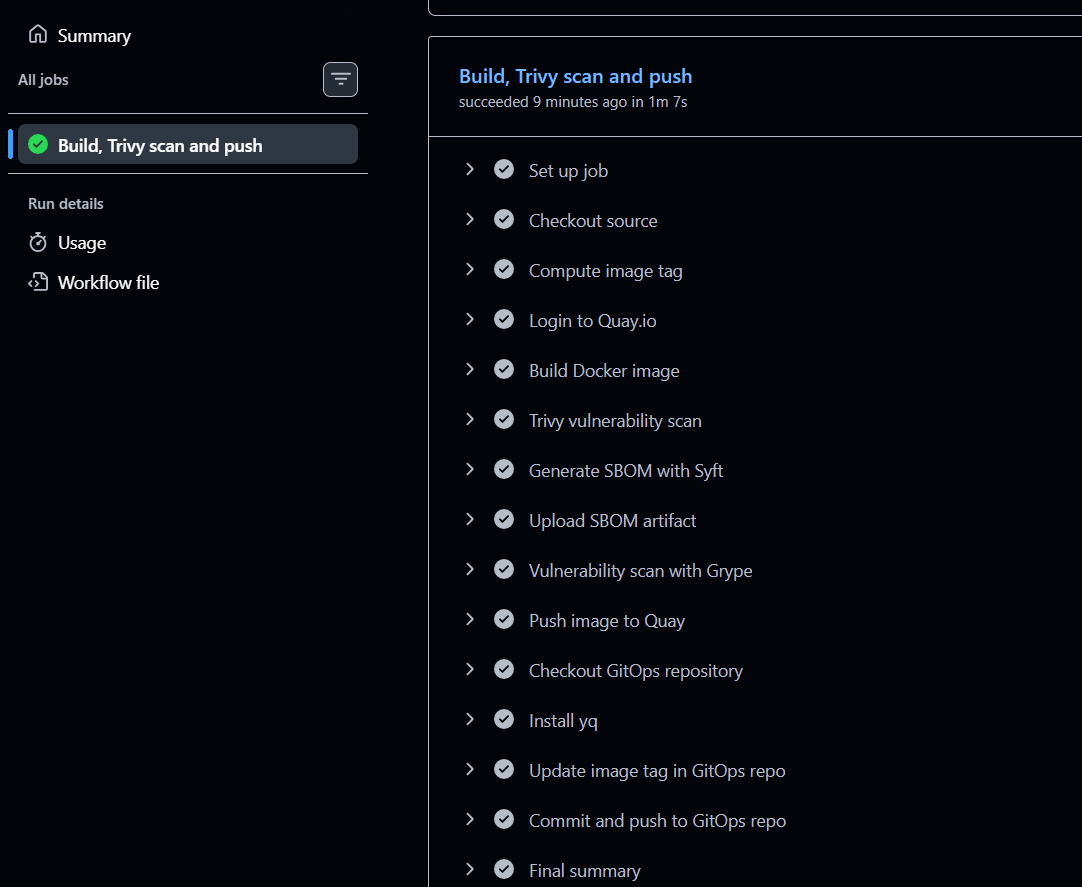
\includegraphics[width=0.70\linewidth]{ci_cd/bloque5_WorkflowCompleto.png}
\caption{Complete \textit{Build, Trivy scan and push} pipeline: the 15 steps of the CI/CD cycle, executed in 1~min~7~s}
\label{fig:ci-workflow-steps-final}
\end{figure}

The step sequence is as follows:

\begin{enumerate}
  \item \textbf{Set up job}: initialisation of the \texttt{ubuntu-latest} runner and download of SHA-referenced actions.
  \item \textbf{Checkout source}: cloning of the \texttt{tfm-demo-app} repository via SHA-pinned \texttt{actions/checkout}.
  \item \textbf{Compute image tag}: computation of the image tag from the first 7 characters of the commit SHA (\texttt{GITHUB\_SHA | cut -c1-7}), exported as \texttt{SHORT\_SHA} and \texttt{FULL\_IMAGE} outputs.
  \item \textbf{Login to Quay.io}: authentication at \texttt{quay.io} with the Robot Account credentials stored in the \texttt{QUAY\_USER} and \texttt{QUAY\_PASSWORD} secrets.
  \item \textbf{Build Docker image}: image build using \texttt{docker/build-push-action} with \texttt{push:\,false}, producing the image in the runner's local daemon without publishing it.
  \item \textbf{Trivy vulnerability scan}: scanning of the local image with Trivy, configured to fail the pipeline on \texttt{HIGH} or \texttt{CRITICAL} severity vulnerabilities (\texttt{ignore-unfixed: true}).
  \item \textbf{Generate SBOM with Syft}: generation of the Software Bill of Materials in syft-json format (Syft's native format \cite{syft_docs}), producing the file \texttt{sbom.syft.json}.
  \item \textbf{Upload SBOM artifact}: upload of the SBOM as a workflow artefact, accessible from the GitHub Actions interface and downloadable for later auditing.
  \item \textbf{Vulnerability scan with Grype}: SBOM analysis with Grype \cite{grype_docs}, configured to fail on \texttt{HIGH} or higher severity with a fix available (\texttt{--only-fixed}).
  \item \textbf{Push image to Quay}: conditional publication of the image to the registry. Only executes if all previous scanning steps have succeeded.
  \item \textbf{Checkout GitOps repository}: cloning of the \texttt{tfm-gitops} repository using the \texttt{GITOPS\_PAT}.
  \item \textbf{Install yq}: installation of \texttt{yq}, the command-line YAML processor.
  \item \textbf{Update image tag in GitOps repo}: update of the \texttt{image} field in the demo application's \texttt{deployment.yaml} manifest.
  \item \textbf{Commit and push to GitOps repo}: commit and push of the updated manifest to the GitOps repository.
  \item \textbf{Final summary}: execution summary.
\end{enumerate}

The first operational version of the pipeline contained only steps 1--6 and 10 (Trivy as the sole scanning engine, without SBOM, Grype, or the GitOps cycle closure). Figure~\ref{fig:ci-workflow-steps-inicial} documents this initial version, with 50~s execution time, which served as the basis for validating the Quay.io integration before adding the SBOM analysis layer.

\begin{figure}[H]
\centering
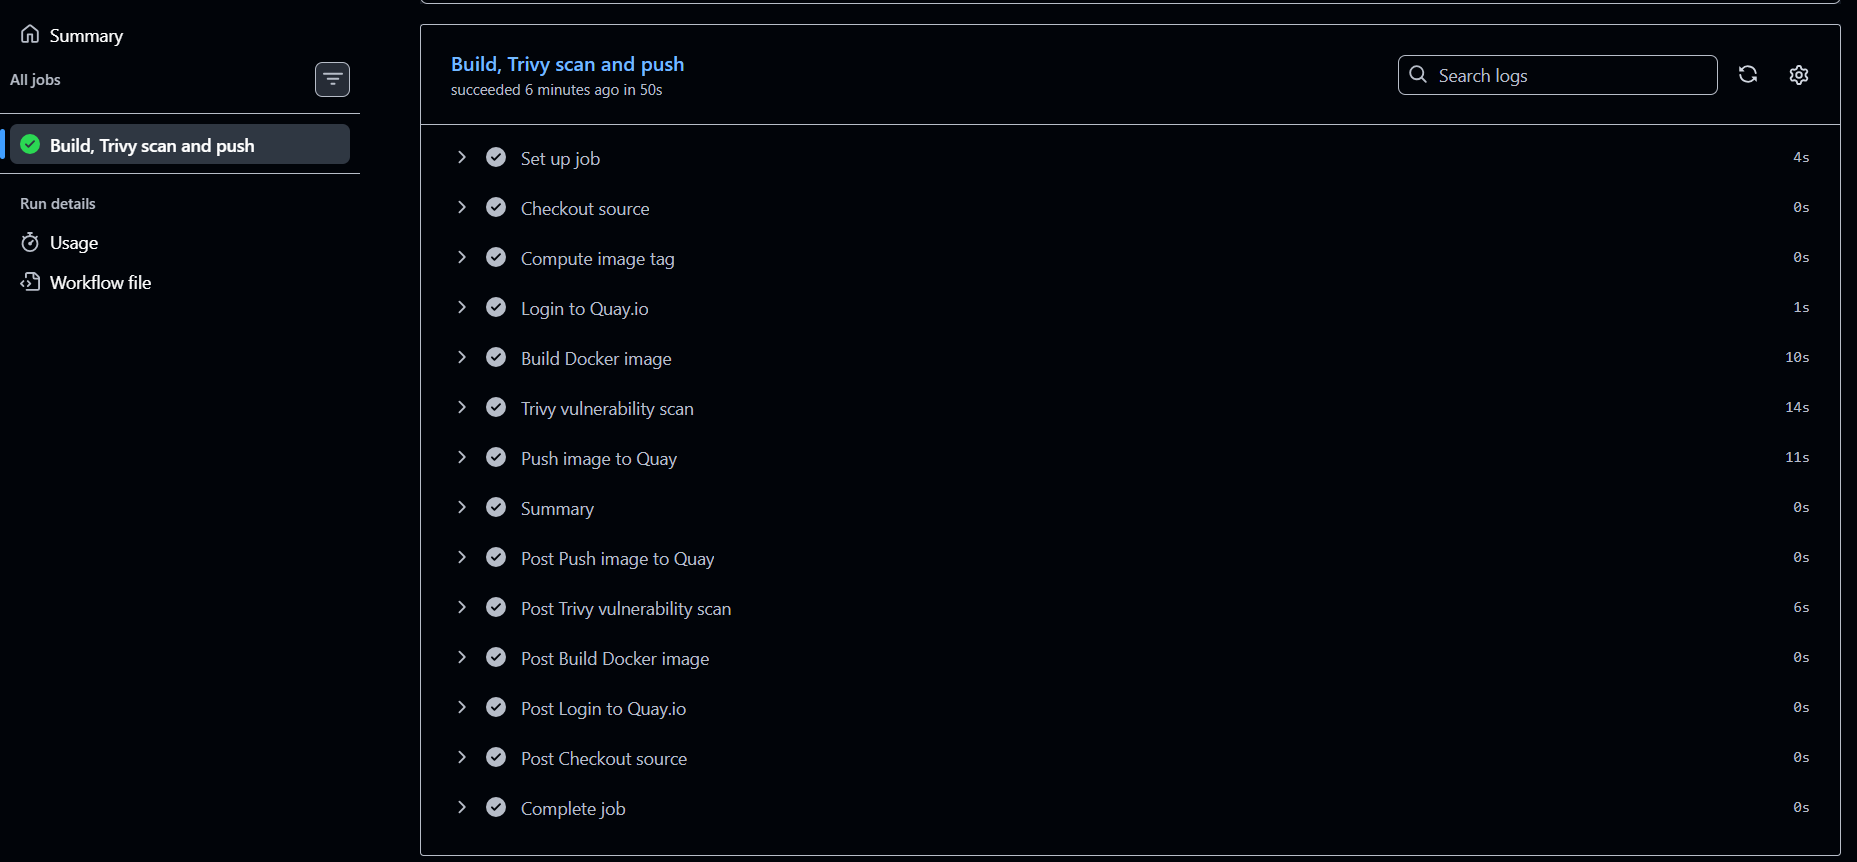
\includegraphics[width=0.90\linewidth]{ci_cd/bloque3_workflowSteps.png}
\caption{Initial version of the \textit{Build, Trivy scan and push} pipeline (without SBOM or Grype): build, Trivy scan and publication steps, completed in 50~s}
\label{fig:ci-workflow-steps-inicial}
\end{figure}

The first successful execution of this pipeline published to Quay.io the image with tag \texttt{4888886} (short SHA of the commit), visible in Figure~\ref{fig:ci-primer-tag}. Quay.io reports for this image 8 medium-severity vulnerabilities and 10 fixable ones, with a size of 47.2~MiB and the manifest SHA256 \texttt{3564a6559cbc}.

\begin{figure}[H]
\centering
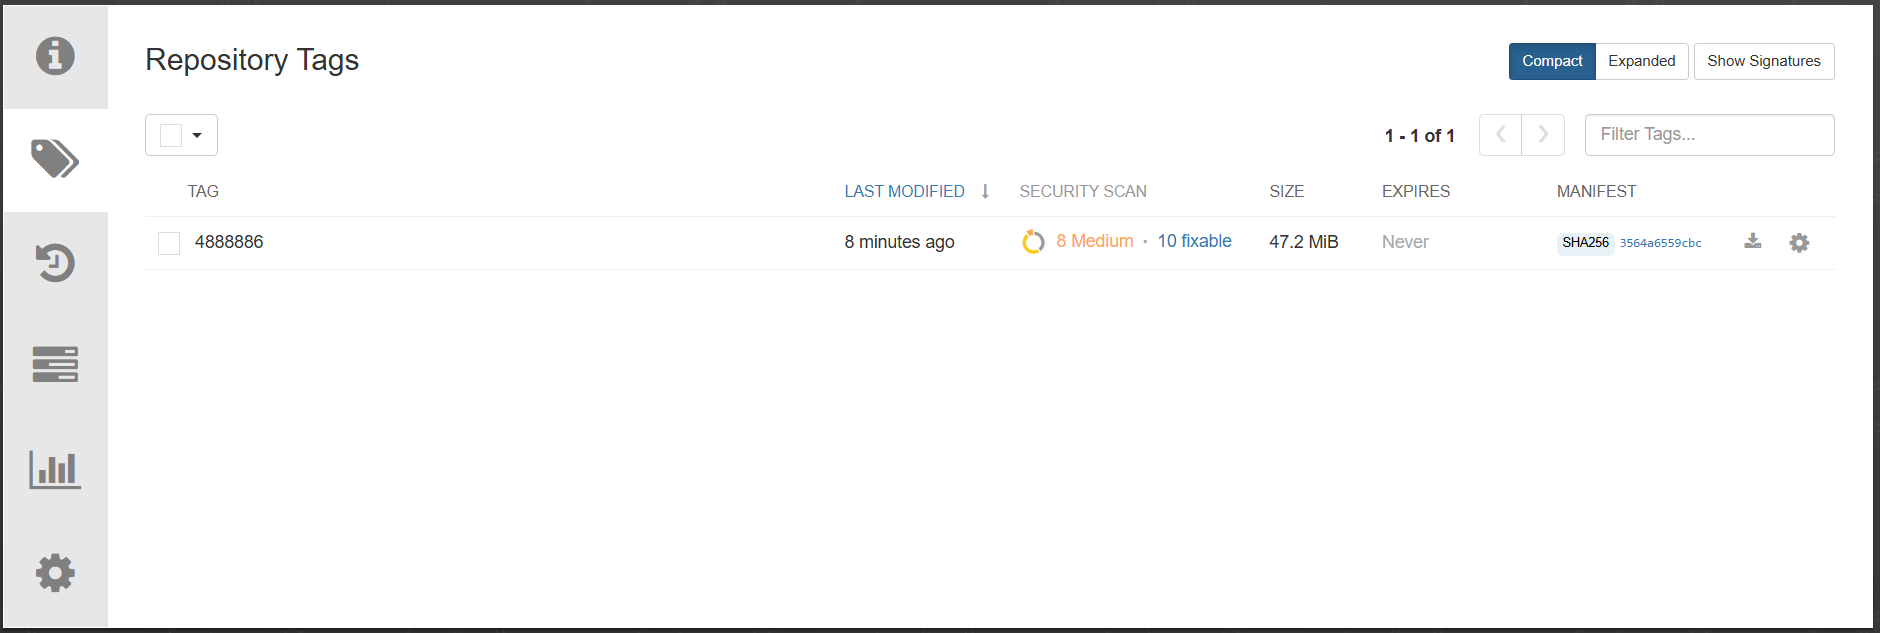
\includegraphics[width=0.90\linewidth]{ci_cd/bloque3_creaccionTag.png}
\caption{First image published to the \texttt{zelkarrabi/tfm-demo-app} Quay.io repository: tag \texttt{4888886} based on the commit short SHA (47.2~MiB)}
\label{fig:ci-primer-tag}
\end{figure}

% ─────────────────────────────────────────────
\section{Vulnerability analysis: defence in depth with Trivy and Grype}
\label{sec:vuln-analysis}
% ─────────────────────────────────────────────

The incorporation of a second vulnerability analysis engine is not a redundancy decision, but one of technical complementarity. To understand why two engines are more secure than one, it is necessary to understand the structural differences between their analysis methodologies and data sources.

\subsection{Complementary scanning architectures}

\textbf{Trivy} \cite{trivy_docs} analyses the image directly, inspecting its layers and extracting installed packages to cross-reference them against its curated database, composed of sources from Aqua Security and the security data repositories of Linux distributions (Red Hat Security Advisories, Debian Security Tracker, Alpine SecDB, among others). Its strength lies in coverage of operating system packages and the speed of its database, which is updated at high frequency.

\textbf{Syft + Grype} operates in two phases. Syft \cite{syft_docs} generates an SBOM of the image, which is a structured and standardised inventory of all artefact components (operating system packages, language libraries, binaries). Grype \cite{grype_docs} analyses that SBOM against its own database, which aggregates sources different from Trivy's: Anchore Enterprise Data, GitHub Security Advisories, National Vulnerability Database (NVD), and Python-specific sources such as the PyPI Advisory Database. This difference in data sources means Grype can detect vulnerabilities that Trivy has not yet incorporated into its database, and vice versa.

\subsection{The SBOM as a compliance deliverable}

Generating the SBOM with Syft is not merely an intermediate step for Grype analysis: the produced file is a \textit{compliance} and traceability artefact with inherent value. An SBOM documents, in a structured and standardised format, which components form part of each artefact, with their exact versions and licences. This inventory allows audit questions to be answered such as: what version of \texttt{urllib3} is in production? which artefacts contain a library affected by a newly published CVE?

There are two main standards for SBOM specification:

\begin{itemize}
  \item \textbf{SPDX} \cite{spdx_spec}: the Linux Foundation standard, primarily oriented toward software licence management and compliance with NIST SSDF \cite{nist_ssdf} software supply chain requirements.
  \item \textbf{CycloneDX} \cite{cyclonedx_spec}: the OWASP Foundation standard, specifically oriented toward security and the DevSecOps lifecycle, with native support for vulnerability analysis and risk metadata.
\end{itemize}

The pipeline emits the SBOM in \textbf{syft-json} format, Syft's native format, which Grype consumes directly for vulnerability analysis. The generated artefact (\texttt{sbom.syft.json}) is uploaded to the workflow under the name \texttt{sbom-\$\{SHORT\_SHA\}}, associating it with the specific run and corresponding image. Unlike SPDX or CycloneDX, syft-json is not a recognised interoperability standard but the tool's internal format; in an environment with formal compliance requirements, the pipeline could additionally emit the SBOM in CycloneDX via \texttt{-o cyclonedx-json}. Figure~\ref{fig:ci-sbom-upload} shows the successful execution of the \textit{Upload SBOM artifact} step: the file \texttt{sbom-defe4ef.zip} was uploaded with a final size of 490,279~bytes (artefact ID \texttt{7196257107}), accessible in the workflow artefacts interface \cite{github_actions_docs}.

\begin{figure}[H]
\centering
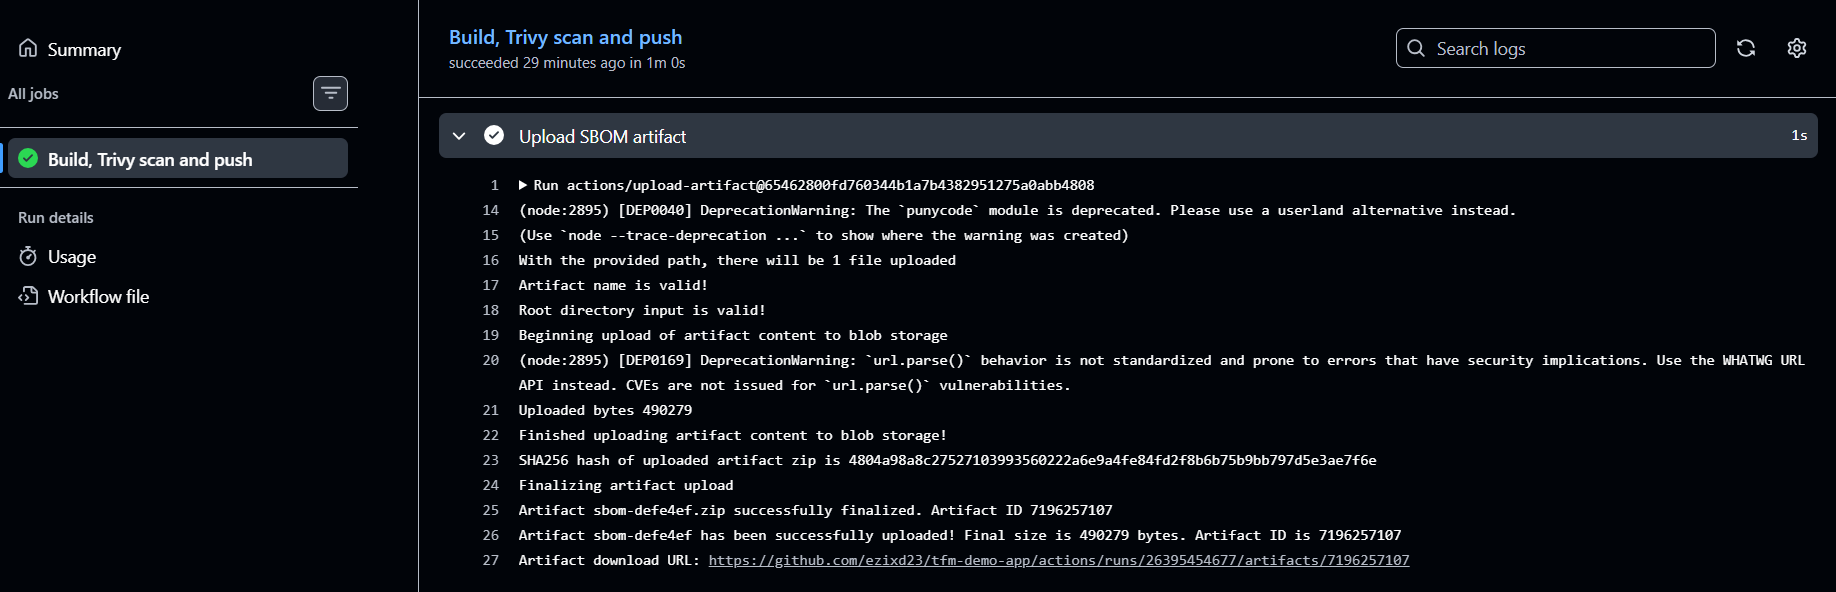
\includegraphics[width=0.95\linewidth]{ci_cd/bloque4_ArtefactoSBOM.png}
\caption{\textit{Upload SBOM artifact} step: upload of \texttt{sbom-defe4ef.zip} as an audit artefact (490,279~bytes, ID~\texttt{7196257107})}
\label{fig:ci-sbom-upload}
\end{figure}

\subsection{Empirical finding: CVE undetected by Trivy, blocking for Grype}

The most relevant empirical finding of the chapter occurred during the first execution of the pipeline with the dual scanning engine active, using the base image \texttt{python:3.12-slim}. Trivy completed its scan without reporting vulnerabilities above the configured severity threshold, and the step advanced correctly. Grype, however, analysed the SBOM generated by Syft and detected vulnerability \textbf{CVE-2025-13836} with \textbf{HIGH} severity in the Python~3.12.13 binary, with fix versions available from \texttt{3.13.11}, \texttt{3.14.1} and \texttt{3.15.0}. The pipeline failed with exit code~1 in the \textit{Vulnerability scan with Grype} step, preventing image publication.

Figure~\ref{fig:ci-grype-output} shows the complete output of the failed step: in addition to CVE-2025-13836 (HIGH), Grype reported multiple MEDIUM-severity vulnerabilities in the Python~3.12.13 binary (CVE-2026-2297, CVE-2026-1299, CVE-2026-0865, CVE-2025-6075, among others) and in the installed Python dependencies (\texttt{flask~3.0.3}, \texttt{pip~25.0.1}, \texttt{werkzeug~3.0.4}). The log closing line, \texttt{Error: Process completed with exit code 1}, confirms that the pipeline stopped at this point, without executing the publication or GitOps repository update steps.

\begin{figure}[H]
\centering
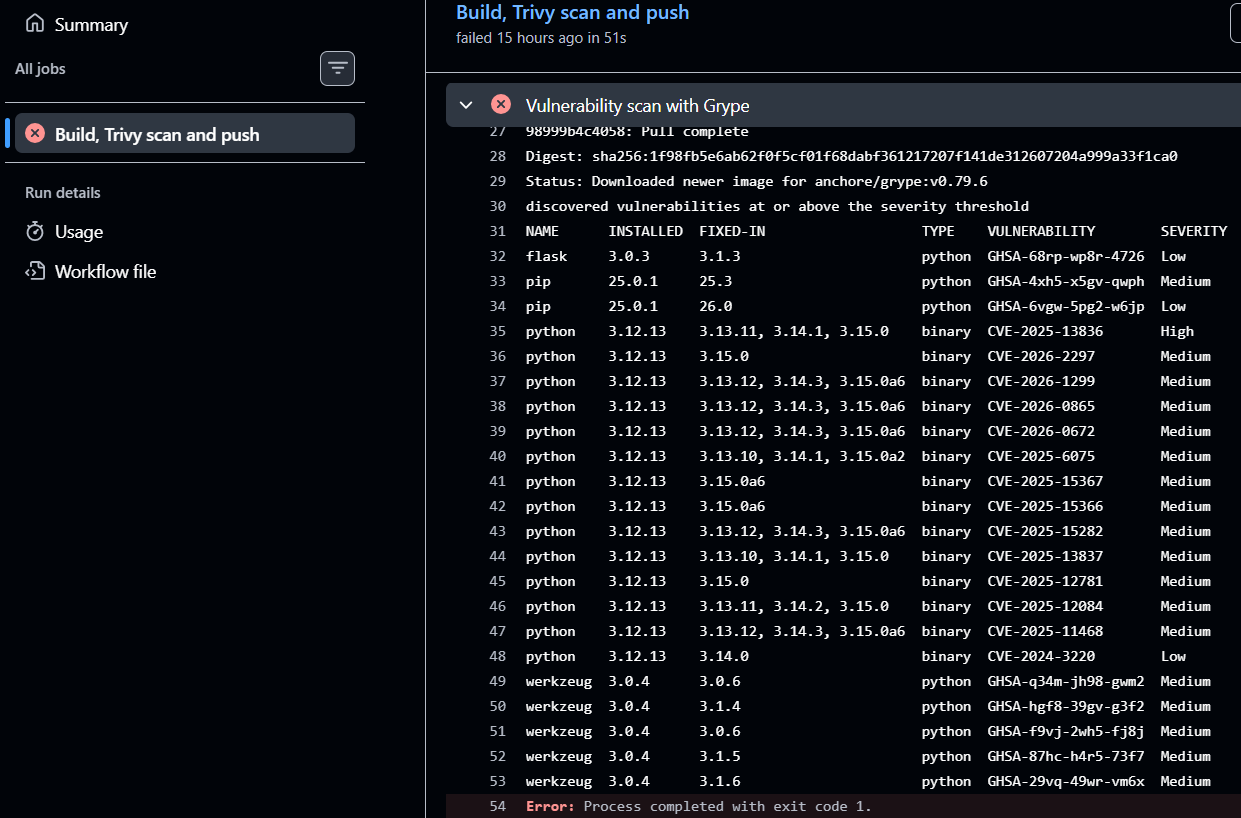
\includegraphics[width=0.95\linewidth]{ci_cd/bloque4_outputTrivyHighPython.png}
\caption{Output of the \textit{Vulnerability scan with Grype} step (\texttt{anchore/grype:v0.79.6}): pipeline blocked by CVE-2025-13836 (HIGH) in \texttt{python~3.12.13}, with fix versions from \texttt{3.13.11}}
\label{fig:ci-grype-output}
\end{figure}

This behaviour is not a failure of either tool. Trivy and Grype have different databases, different severity taxonomies, and independent rates of incorporating new CVEs. CVE-2025-13836 was present in Grype's database at the time of execution but not in Trivy's. This temporal lag between databases is a known and documented phenomenon in the container security literature \cite{nist_sp800190}: organisations that rely on a single scanning engine implicitly assume that engine has complete coverage of all relevant CVEs, an assumption this experiment refutes empirically.

The conclusion is precisely the inverse: diversity of analysis engines provides real security layers because each engine can detect CVEs that others have not yet incorporated. The defence-in-depth principle, typically applied at the cluster access control and configuration layer (Kyverno as the admission engine, ArgoCD as the declarative state controller), is applied here to the image supply chain layer: no scanning engine is sufficient on its own.

It is worth, however, bounding the scope of the finding. CI scanning is \textit{point-in-time}: it only detects vulnerabilities present in the databases at the time of the build; a CVE published after the image has been built and published will go unnoticed until the next cycle. This makes periodic re-scanning of already published images and runtime monitoring indispensable---a function that in the Chapter~5 architecture corresponds to Sysdig. Additionally, the defence-in-depth conclusion rests on a single empirical case in which the engines employed different severity taxonomies; in scenarios where both taxonomies are aligned, the coverage difference between engines may be smaller.

% ─────────────────────────────────────────────
\section{Technical incidents and lessons learned}
% ─────────────────────────────────────────────

This section documents the three most relevant technical incidents that arose during pipeline implementation. Like the lessons-learned sections of Chapters~6 and~7, the objective is not to narrate failures, but to extract technical conclusions of value that illustrate general principles of secure CI/CD system design.

\subsection{Incident 1: supply chain attack on the Trivy action itself}

The first incident affected the very defence mechanism designed to protect the pipeline from supply chain attacks: SHA-based version pinning of actions. Despite referencing \texttt{aquasecurity/trivy-action} by its full SHA hash, the pipeline failed on the first execution attempt with an action resolution error.

The root cause, identified after analysing the runner logs, was that \texttt{aquasecurity/trivy-action} has an internal transitive dependency on an auxiliary action named \texttt{setup-trivy}, referenced via a mutable tag (not SHA-pinned). Aqua Security had removed or relocated this tag as part of a response to a security incident in their own infrastructure, which broke the action resolution chain even though the SHA of the main action remained intact.

Figure~\ref{fig:ci-workflow-inicial} shows the history of the first two workflow executions: the first (\textit{feat: initial application code, Dockerfiles and CI workflow}, commit \texttt{6070383}) failed in 7~s for this reason; the second (\textit{ci: update trivy-action SHA to fix broken transitive dependency}, commit \texttt{4888886}) succeeded in 52~s after updating to the SHA corresponding to the stable \texttt{v0.35.0} version.

\begin{figure}[H]
\centering
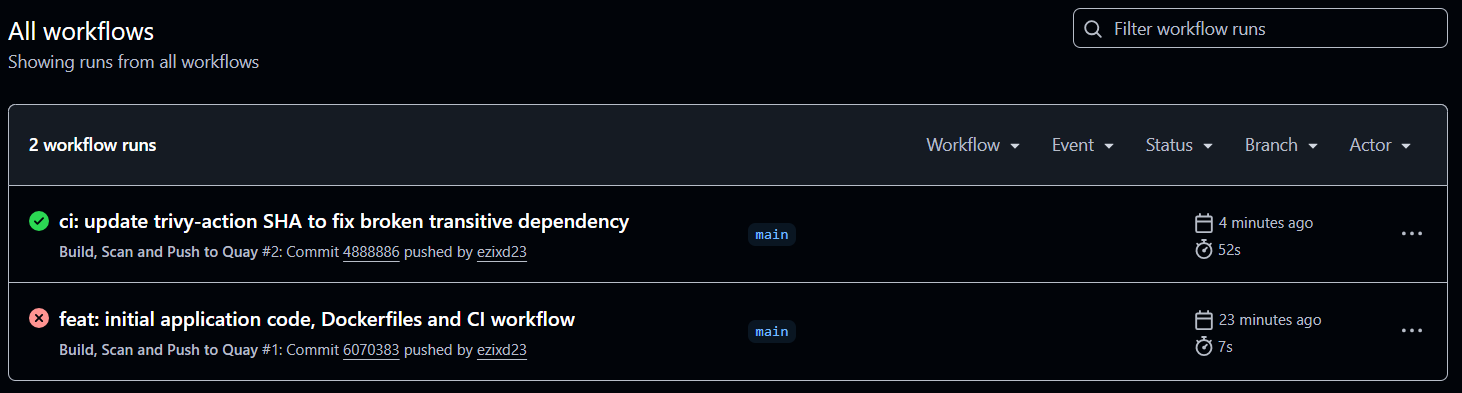
\includegraphics[width=0.95\linewidth]{ci_cd/bloque3_workflowActions.png}
\caption{Initial workflow history: failure of run~\#1 (7~s) due to a broken transitive dependency in the Trivy action, and correction in run~\#2 (52~s) with the \texttt{v0.35.0} SHA}
\label{fig:ci-workflow-inicial}
\end{figure}

This incident empirically demonstrates a real limitation of supply chain security in CI systems based on third-party components: SHA pinning protects only against mutation of the directly referenced action code, but not against transitive dependencies that the action may resolve internally via mutable tags. In a production environment, complete mitigation would require either that action providers also pin their internal dependencies by SHA, or the use of a \textit{vendoring} system that internalises all dependencies in the corporate repository. The pragmatic solution adopted---updating to the SHA of the stable version with active support---is an acceptable compromise that restores pipeline immutability for the most recent version of the action.

\subsection{Incident 2: reproducibility versus Grype database freshness}

The second incident affected the \textit{Vulnerability scan with Grype} step after the SBOM was incorporated. By pinning the Grype image version as \texttt{anchore/grype:v0.79.6}, the vulnerability database included in that image was static and dated from the image's publication date. By default, Grype validates that its CVE database is no more than 5~days old; if the threshold is exceeded, Grype fails with an error before processing the SBOM.

This behaviour exposes a fundamental \textit{trade-off} in security pipeline design: \textbf{reproducibility} (pinned image version, deterministic pipeline behaviour) conflicts with \textbf{database currency} (coverage of the most recent vulnerabilities). Prioritising reproducibility means the pipeline will always use the same version of Grype with the same database, but that database becomes obsolete over time. Prioritising database currency means the Grype image updates automatically, but introduces variability in pipeline behaviour (a run may fail not because the image has new vulnerabilities, but because the updated database incorporates new entries).

The adopted solution was to configure the environment variable \texttt{GRYPE\_DB\_VALIDATE\_AGE=false}, which instructs Grype to skip age validation and use the database available in the pinned image:

\begin{lstlisting}
- name: Vulnerability scan with Grype
  run: |
    docker run --rm \
      -e GRYPE_DB_VALIDATE_AGE=false \
      -v "$PWD":/work \
      anchore/grype:v0.79.6 \
      sbom:/work/sbom.syft.json \
      --fail-on high \
      --only-fixed
\end{lstlisting}

This decision prioritises pipeline determinism: the same workflow with the same inputs will always produce the same behaviour, facilitating incident debugging and result reproduction. In a production environment, the recommended alternative would be a controlled periodic renewal of the Grype image version through a managed update process (weekly automatic pull request, for example), combining database updates with an explicit review before being incorporated into the pipeline.

Figure~\ref{fig:ci-workflow-sbom-iteraciones} documents the complete workflow execution history during the resolution of this incident: runs \#3, \#4 and \#5 correspond to the attempts to resolve the Grype database problem, until reaching the stable solution with \texttt{GRYPE\_DB\_VALIDATE\_AGE=false} in run \#6.

\begin{figure}[H]
\centering
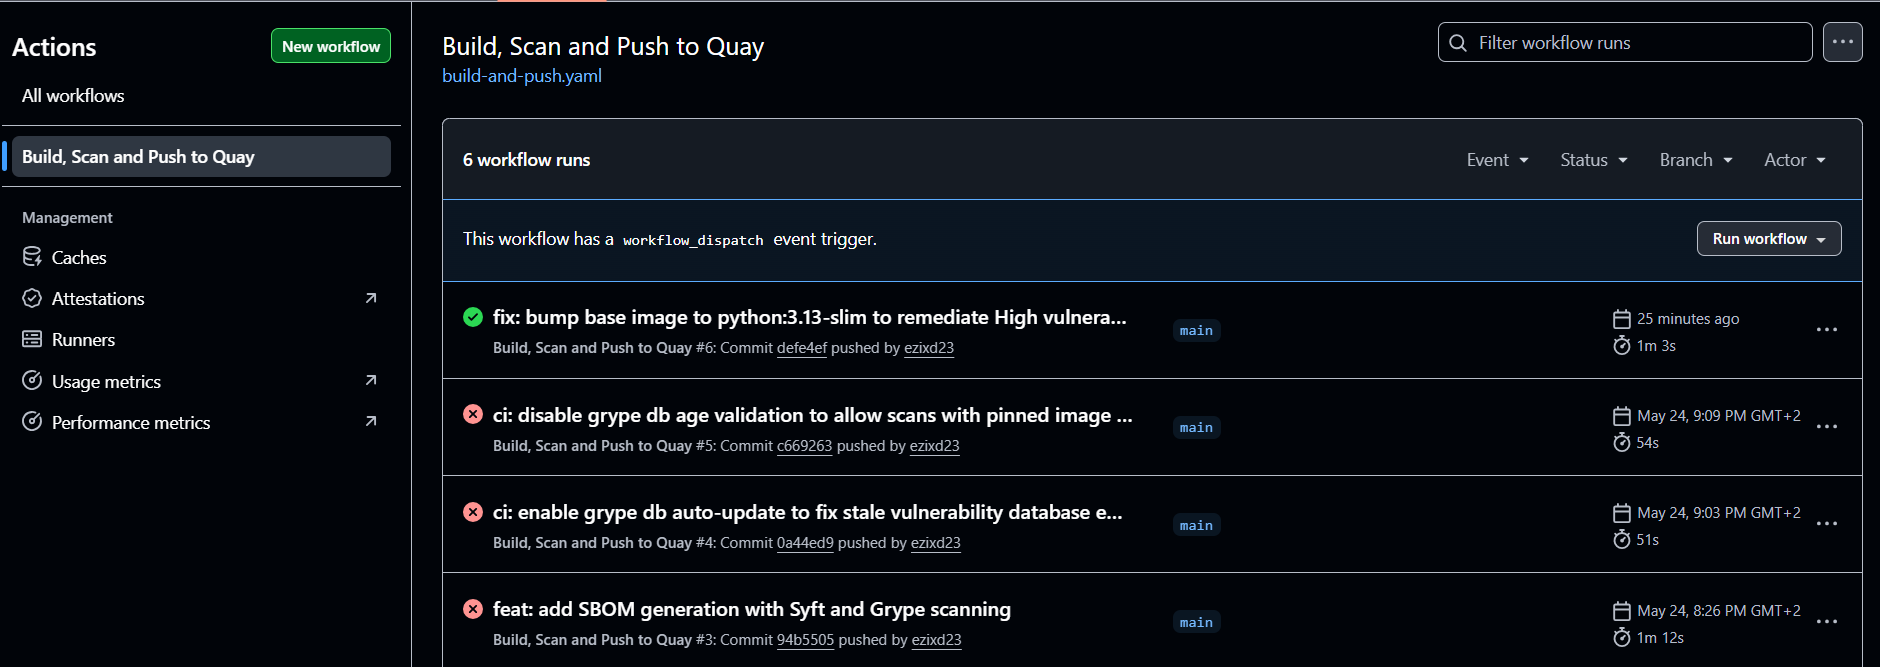
\includegraphics[width=0.95\linewidth]{ci_cd/bloque4_flujoWorkflowAlIncluirSBOMGrype.png}
\caption{Workflow \textit{Build, Scan and Push to Quay} history: incident resolution iterations with SBOM and Grype (runs \#3--\#5 failed) and final successful execution with \texttt{python:3.13-slim} (run \#6, commit \texttt{defe4ef})}
\label{fig:ci-workflow-sbom-iteraciones}
\end{figure}

\subsection{Incident 3: applying the Shift-Left principle against CVE-2025-13836}

The third incident is, in terms of academic value, the most representative of the chapter: the pipeline blocked the publication of the \texttt{python:3.12-slim} image due to CVE-2025-13836 (HIGH) detected by Grype, as documented in Section~\ref{sec:vuln-analysis}. Faced with this block, there were two response paths:

\begin{enumerate}
  \item Reduce the Grype severity threshold from \texttt{HIGH} to \texttt{CRITICAL}, so that CVE-2025-13836 would not block the pipeline.
  \item Fix the vulnerability at the source by updating the base image to a Python version that does not contain the CVE.
\end{enumerate}

The first option was evaluated and rejected because it would compromise the system's security standards: a HIGH-severity vulnerability in the Python runtime is not a false positive or an acceptable risk in a DevSecOps environment, and relaxing the detection threshold would be equivalent to systematically ignoring every vulnerability that does not reach maximum criticality. The second option, updating the base image to \texttt{python:3.13-slim}, resolves the problem at the source without compromising any control.

This decision exemplifies the \textit{Shift-Left} principle \cite{sharma2020devsecops}: instead of managing the vulnerability at the deployment layer (adding exceptions or relaxing controls), it is corrected at the earliest possible phase of the lifecycle---the selection of the Dockerfile base image. The pipeline is not just a vulnerability detector; it is a mechanism that imposes an obligation to fix at the source before the artefact advances through the chain.

The fix was applied in commit \texttt{defe4ef} (\textit{fix: bump base image to python:3.13-slim to remediate High vulnerability}). The resulting image, published to Quay.io under the same tag, has 7 medium-severity vulnerabilities and 8 fixable ones with a size of 46.9~MiB---a reduction in both the number of CVEs and the image size, as expected when using a more modern and patched version of Python.

\textbf{Note on the Dockerfilevulnerable.} The blocking scenario that \texttt{Dockerfilevulnerable} (based on \texttt{python:\allowbreak{}3.4-alpine}) would have allowed reproducing artificially proved unnecessary: the development pipeline itself produced a verified genuine test by legitimately blocking an image the team considered secure at the time (\texttt{python:3.12-slim}). This real-world test has greater academic value than an artificial one because it demonstrates the system working in a production scenario where vulnerabilities emerge without warning: the developer did not deliberately choose an insecure image, nor was the block prepared. The CVE was present in Grype's database, the image contained it, and the pipeline did exactly what it was designed to do.

% ─────────────────────────────────────────────
\section{Closing the CI/CD cycle: integration with the GitOps repository}
% ─────────────────────────────────────────────

The final block of the pipeline closes the CI/CD cycle, connecting the Continuous Integration layer documented in this chapter with the Continuous Deployment layer implemented in Chapter~7. Once all security controls have been passed and the image published to Quay.io, the pipeline updates the GitOps repository automatically.

\subsection{Automatic GitOps repository update}

The update process is performed in four consecutive workflow steps:

\textbf{Checkout GitOps repository.} The pipeline checks out the \texttt{tfm-gitops} repository using the \texttt{GITOPS\_PAT}:

\begin{lstlisting}
- name: Checkout GitOps repository
  uses: actions/checkout@b4ffde65f46336ab88eb53be808477a3936bae11  # v4.1.1
  with:
    repository: ezixd23/tfm-gitops
    token: ${{ secrets.GITOPS_PAT }}
    path: gitops-repo
    ref: main
\end{lstlisting}

Using \texttt{GITOPS\_PAT} instead of the default \texttt{GITHUB\_TOKEN} is a technically justified decision: the \texttt{GITHUB\_TOKEN} has permissions only over the repository in which the workflow runs (\texttt{tfm-demo-app}) and cannot write to a different repository. The \texttt{GITOPS\_PAT} is the necessary mechanism for cross-repository writes; in production it should be a fine-grained PAT limited to \texttt{tfm-gitops} with \texttt{Contents: read/write}, as reasoned in Section~8.2.

\textbf{Install yq.} \texttt{yq}, Mike Farah's command-line YAML processor, is installed to allow modifying specific fields of a YAML file without altering the rest of the file's structure.

The choice of \texttt{yq} over alternatives such as \texttt{sed} is based on robustness considerations. \texttt{sed} operates on plain text without understanding YAML structure: a format change in the file (different spacing, comments, field reordering) can silently break the substitution regular expression, producing a malformed manifest. \texttt{yq}, by processing YAML as a structured data tree, guarantees that only the \texttt{image} field of the first container of the Deployment is modified, preserving the rest of the file unchanged.

\textbf{Update image tag in GitOps repo.} The manifest update is performed with a \texttt{yq} expression that navigates the Deployment structure:

\begin{lstlisting}
- name: Update image tag in GitOps repo
  run: |
    cd gitops-repo
    yq eval -i \
      ".spec.template.spec.containers[0].image = \"${{ steps.vars.outputs.FULL_IMAGE }}\"" \
      applications/demo-app/deployment.yaml
\end{lstlisting}

\textbf{Commit and push to GitOps repo.} The commit includes a message with cross-repository traceability:

\begin{lstlisting}
- name: Commit and push to GitOps repo
  run: |
    cd gitops-repo
    git config user.name "GitHub Actions CI"
    git config user.email "actions@github.com"
    git add applications/demo-app/deployment.yaml
    git commit -m "chore: update demo-app image to ${{ steps.vars.outputs.SHORT_SHA }}"
    git push origin main
\end{lstlisting}

The commit message includes the image short SHA (\texttt{steps.vars.outputs.SHORT\_SHA}), enabling bidirectional auditing: given a commit in \texttt{tfm-gitops}, it is possible to identify the deployed image tag, and given an image tag in Quay.io, it is possible to locate the source code commit that originated it.

\subsection{Empirical evidence of the complete cycle}

Figure~\ref{fig:ci-git-log} shows the commit history in the \texttt{tfm-gitops} repository after the complete pipeline execution. The most recent commit (\texttt{f762c09}, \texttt{HEAD}) has the message \texttt{chore: update demo-app image to d8ae0bd}, direct evidence that the pipeline automatically updated the GitOps repository with the new image tag.

\begin{figure}[H]
\centering
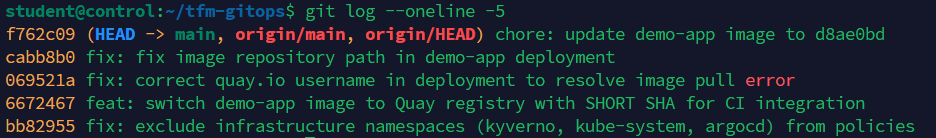
\includegraphics[width=0.90\linewidth]{ci_cd/bloque5_logDeCommitAutomatico.png}
\caption{Commit history in \texttt{tfm-gitops}: the automatic commit \texttt{f762c09} updates the image tag to \texttt{d8ae0bd}, triggering ArgoCD synchronisation}
\label{fig:ci-git-log}
\end{figure}

Once this new commit is detected by ArgoCD through its repository polling mechanism (and its continuous watch over synchronised cluster resources described in Section~7.5.1), the reconciliation controller initiates synchronisation of the \texttt{Deployment} with the new image specification. Figure~\ref{fig:ci-quay-tags} shows the history and status of the image repository in Quay.io, where four tags published by different pipeline runs are now visible: \texttt{d8ae0bd} as the most recent image (46.9~MiB), alongside previous versions \texttt{036fe39}, \texttt{defe4ef} (image with \texttt{python:3.13-slim}, 46.9~MiB) and \texttt{4888886} (initial image with \texttt{python:3.12-slim}, 47.2~MiB).

\begin{figure}[H]
\centering
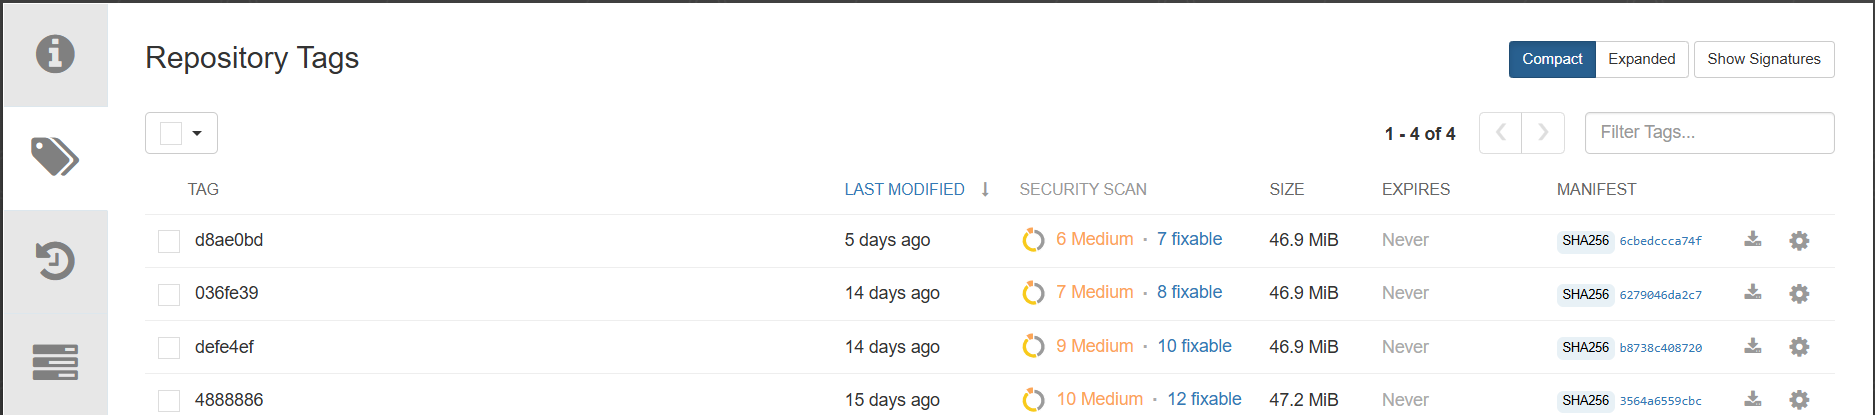
\includegraphics[width=0.95\linewidth]{ci_cd/bloque4_nuevoTAG.png}
\caption{Repository \texttt{zelkarrabi/tfm-demo-app} on Quay.io showing the history of the four tags published by the pipeline, with \texttt{d8ae0bd} as the most recent and secure image.}
\label{fig:ci-quay-tags}
\end{figure}

Figure~\ref{fig:ci-pod-image} shows the final verification from the cluster: the two pods of the \texttt{demo-app} Deployment in \texttt{Running} state are executing the image \texttt{quay.io/zelkarrabi/tfm-demo-app:d8ae0bd}, the tag based on the short SHA of the last commit that passed all pipeline controls.

\begin{figure}[H]
\centering
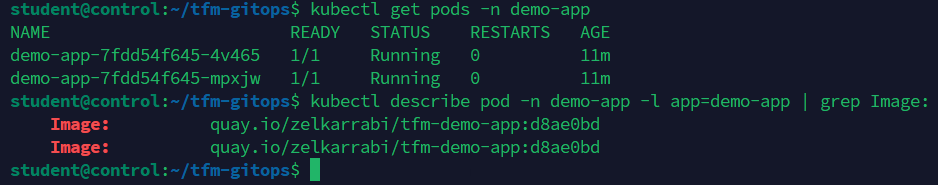
\includegraphics[width=0.90\linewidth]{ci_cd/bloque5_podConImagenActualizada.png}
\caption{Cluster verification: the two \texttt{demo-app} pods in \texttt{Running} state with image \texttt{quay.io/zelkarrabi/\allowbreak{}tfm-demo-app:d8ae0bd} deployed by ArgoCD}
\label{fig:ci-pod-image}
\end{figure}

The ArgoCD interface pod view, shown in Figure~\ref{fig:ci-argocd-pod}, presents the full detail of pod \texttt{demo-app-86d6c6d8f7-8s9c6} created on 06/03/2026 at 13:45:41: the active image is \texttt{quay.io/zelkarrabi/tfm-demo-app@sha256:6279046da2c79968\ldots}, the container state is \texttt{Running} (\textit{started and ready}) and the pod health is \texttt{Healthy}. The SHA256 digest reference appearing in the pod's \texttt{imageID} field is not resolved by ArgoCD: it is the kubelet that, at pull time, downloads the tag-referenced image and records the exact digest of the downloaded manifest; ArgoCD merely reflects that live value from the pod state. The practical result is effective immutability: even if the tag were redirected in the registry to a different image, the running pod has already fixed the digest in its \texttt{imageID}.

\begin{figure}[H]
\centering
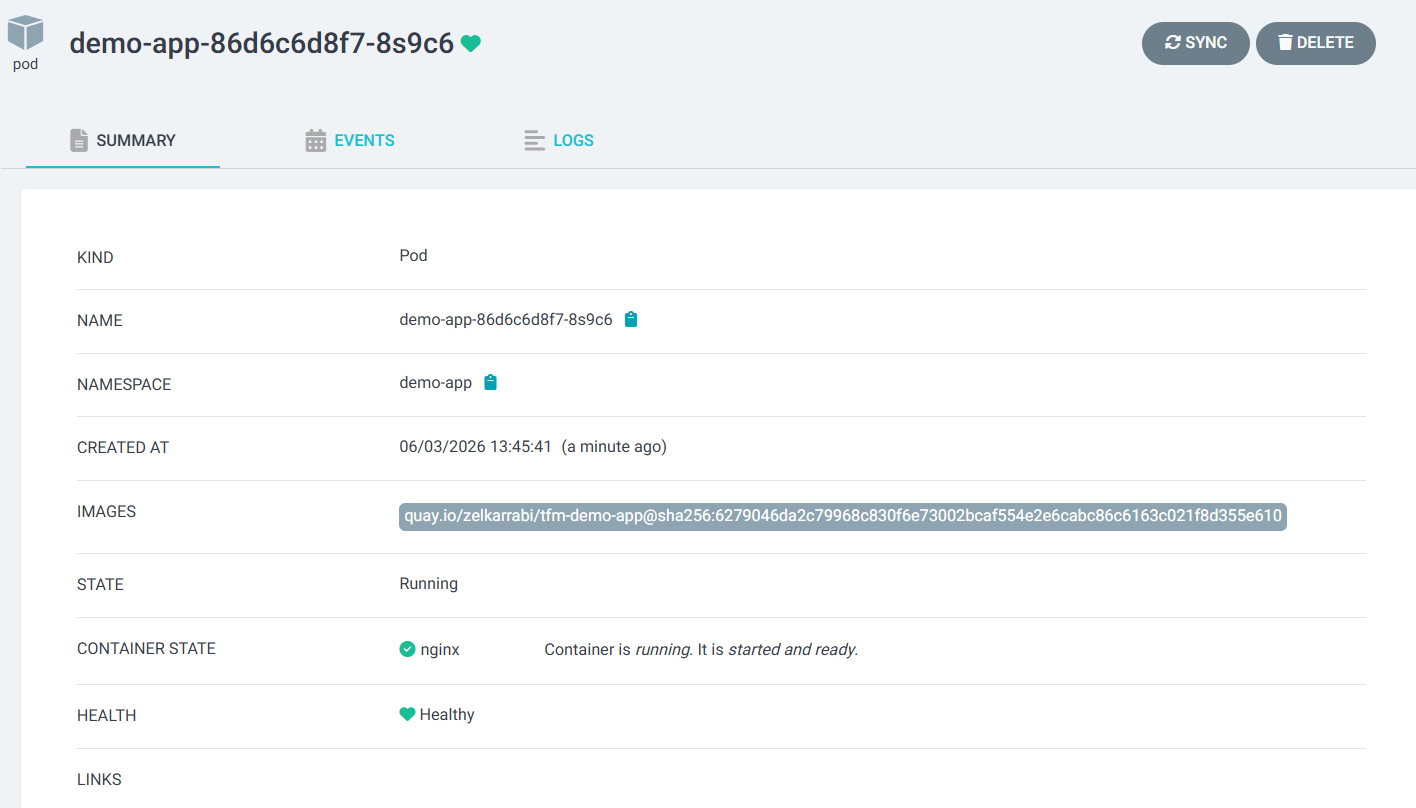
\includegraphics[width=0.85\linewidth]{ci_cd/bloque5_actualizadoImagenQuaypng.png}
\caption{Detail of pod \texttt{demo-app-86d6c6d8f7-8s9c6} in ArgoCD: active image referenced by SHA256 digest, \texttt{Running} state and \texttt{Healthy} health}
\label{fig:ci-argocd-pod}
\end{figure}

The final end-to-end test consists of verifying that the change introduced in the \texttt{tfm-demo-app} source code is visible in the HTTP response of the application deployed in the cluster. Figure~\ref{fig:ci-curl-end-to-end} shows the application response accessed at \texttt{192.168.1.101:8888}: the returned JSON object includes the field \texttt{ci\_pipeline:\,"end-to-end-test"}, the value of the \texttt{CI\_PIPELINE} environment variable configured in the Deployment, which confirms that the deployed code corresponds exactly to the commit that activated the pipeline. The field \texttt{hostname:\,demo-app-7fdd54f645-4d5nk} identifies the specific pod that served the request, and \texttt{service:\,tfm-demo-app} and \texttt{version:\,1.0.0} correspond to the values declared in the application source code.

\begin{figure}[H]
\centering
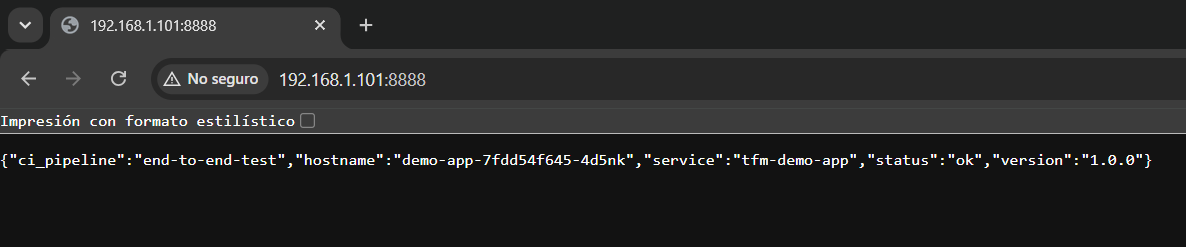
\includegraphics[width=0.80\linewidth]{ci_cd/bloque5_curlMostrandoCambioCodigoFuente.png}
\caption{HTTP response from the application at \texttt{192.168.1.101:8888}: the \texttt{ci\_pipeline:\,end-to-end-test} field confirms the complete propagation of the source code change to the runtime environment}
\label{fig:ci-curl-end-to-end}
\end{figure}

\subsection{The complete DevSecOps cycle}

The combination of the results documented in this chapter and Chapter~7 constitutes the complete materialisation of the DevSecOps architecture designed in Chapter~5. The end-to-end flow empirically verified is as follows:

\begin{enumerate}
  \item A developer makes a change to the \texttt{tfm-demo-app} source code and pushes to the \texttt{main} branch.
  \item GitHub Actions detects the event and launches the \textit{Build, Scan and Push to Quay} workflow.
  \item The pipeline builds the Docker image with the multi-stage Dockerfile and non-root user.
  \item Trivy scans the image; if any \texttt{HIGH} or \texttt{CRITICAL} vulnerability with a fix available is detected, the pipeline fails here.
  \item Syft generates the image SBOM and uploads it as a permanent audit artefact.
  \item Grype analyses the SBOM; if any HIGH or higher severity vulnerability is detected, the pipeline fails here.
  \item The image, free of vulnerabilities above the threshold, is published to Quay.io under the commit short SHA tag.
  \item The pipeline updates the \texttt{image} field of the Deployment in \texttt{tfm-gitops} via \texttt{yq} and commits with cross-repository traceability.
  \item ArgoCD detects the new commit in \texttt{tfm-gitops} through its watch on synchronised resources and its Git polling cycle, and synchronises the Deployment with the new image.
  \item Kubernetes creates the new pods; Kyverno intercepts the creation request, applies the mutation policies (P4--P7) and validates against the validation policies (P1--P3, P9). If the pod does not satisfy any condition not fixable through mutation, it is rejected.
  \item The new pods transition to \texttt{Running} state and the application responds HTTP with the values from the new source code.
\end{enumerate}

This flow integrates the three layers of the DevSecOps architecture from Chapter~5: the development layer (source code and Git), the automation layer (GitHub Actions and ArgoCD), and the execution layer (Kubernetes with Kyverno). Security is integrated at every transition between layers: Trivy and Grype between the development layer and the image registry; Kyverno policies between the registry and the cluster; and ArgoCD as the guarantor that the cluster state remains aligned with the configuration repository.

With the complete CI/CD cycle implemented and empirically verified, the next chapter addresses the practical comparison between Kyverno and OPA Gatekeeper, which complements the theoretical review of Chapter~2 with evidence obtained through the direct reimplementation of a representative subset of the Chapter~6 policies in OPA's Rego language.

\chapter{Practical Comparison Between Kyverno and OPA Gatekeeper}

Chapter~2 presented in Section~2.5 a theoretical comparison between Kyverno and OPA Gatekeeper, synthesised in Table~2.1. This chapter complements that view with practical evidence: the reimplementation in the Rego language \cite{rego_docs} of a representative subset of the Chapter~6 policies, covering the three engine mechanisms---validation, mutation, and generation---so that the differences in syntax, object model, and capabilities can be analysed on real code.

The comparison is conducted at the code level, without deploying OPA Gatekeeper in the cluster. This approach is justified by two technical reasons. First, the coexistence of two admission controllers in the same cluster is operationally problematic: both Kyverno and Gatekeeper register \texttt{MutatingWebhookConfiguration} and \texttt{ValidatingWebhookConfiguration} that would intercept the same admission requests, potentially generating confusing behaviour, duplicate error messages, and additional load on the API Server. Second, the lab environment used in this work (two virtual machines with shared resources) hosts an already operational Kubernetes cluster with Kyverno, ArgoCD, and the CI pipeline functional; adding a second admission engine without impacting environment stability is not viable. Code-level comparison is therefore the appropriate methodology for this context.

The chapter is organised into five sections. The first describes the Gatekeeper object model to contextualise the comparison. The second and third sections compare concrete implementations of validation and mutation policies respectively. The fourth documents the absence of a Gatekeeper equivalent for the generation capability. The fifth synthesises the findings and justifies the choice of Kyverno for the DevSecOps environment of this work.

% ─────────────────────────────────────────────
\section{The OPA Gatekeeper model}
% ─────────────────────────────────────────────

OPA Gatekeeper \cite{gatekeeper_docs} is an admission controller for Kubernetes that externalises policy evaluation to the OPA (\textit{Open Policy Agent}) engine \cite{opa_docs}. Unlike Kyverno, whose policies are expressed as native Kubernetes YAML manifests, Gatekeeper requires the Rego language \cite{rego_docs}---a general-purpose declarative language based on first-order logic---to express the evaluation logic.

The Gatekeeper object model is based on two separate resources per policy. The \textbf{ConstraintTemplate} defines the policy logic in Rego and, when applied to the cluster, dynamically generates a new CRD (Custom Resource Definition) type whose name the author determines. The \textbf{Constraint} instantiates that CRD type for a specific configuration: it defines which resources the policy applies to (via the \texttt{match} field), which namespaces to exclude, and optionally passes parameters to the Rego code. Kyverno, by contrast, condenses both aspects---the logic and the application configuration---into a single \texttt{ClusterPolicy} object.

Mutation in Gatekeeper \cite{gatekeeper_mutation} is a separate component from the validation core, independently enabled and based on its own object types (\texttt{Assign}, \texttt{AssignMetadata}) that use a location syntax different from the Rego used for validation. This architectural separation has relevant practical implications that are analysed in Section~9.3.

% ─────────────────────────────────────────────
\section{Comparison in validation policies}
% ─────────────────────────────────────────────

\subsection{Policy P1: \texttt{disallow-root}}

The first policy prevents the deployment of pods that do not declare \texttt{runAsNonRoot:\,true} in their \texttt{securityContext}. Its Kyverno implementation---a single \texttt{ClusterPolicy} with a \texttt{pattern} requiring that field---is documented in Section~6.3.1. The equivalent Gatekeeper implementation requires two objects. The \texttt{ConstraintTemplate} contains the logic in Rego:

\begin{lstlisting}
# Gatekeeper - ConstraintTemplate (object 1/2)
apiVersion: templates.gatekeeper.sh/v1
kind: ConstraintTemplate
metadata:
  name: k8sdisallowroot
spec:
  crd:
    spec:
      names:
        kind: K8sDisallowRoot
  targets:
    - target: admission.k8s.gatekeeper.sh
      rego: |
        package k8sdisallowroot

        violation[{"msg": msg}] {
          not input.review.object.spec.securityContext.runAsNonRoot == true
          msg := "Containers must not run as root"
        }
\end{lstlisting}

The \texttt{Constraint} instantiates the above template for the \texttt{Pod} type:

\begin{lstlisting}
# Gatekeeper - Constraint (object 2/2)
apiVersion: constraints.gatekeeper.sh/v1beta1
kind: K8sDisallowRoot
metadata:
  name: disallow-root
spec:
  match:
    kinds:
      - apiGroups: [""]
        kinds: ["Pod"]
    excludedNamespaces:
      - kyverno
      - kube-system
      - argocd
\end{lstlisting}

The comparison highlights two fundamental differences. The first is the \textbf{inversion of the logical paradigm}: Kyverno expresses the \textit{desired state} (the \texttt{runAsNonRoot} field must be \texttt{true}), and the engine rejects any resource that does not match that pattern. Rego, by contrast, expresses the \textit{violation condition} (the negation of the correct state), and OPA executes that rule to determine whether an infraction exists. A developer reading the Kyverno policy directly sees what a pod must satisfy; a developer reading the Rego needs to mentally invert the condition to infer the requirement. The second difference is the \textbf{object count}: Kyverno resolves the policy in a single object of approximately 20 lines; Gatekeeper requires two objects totalling approximately 30 lines.

One aspect where Gatekeeper presents a conciseness advantage that must be acknowledged explicitly is \textbf{namespace exclusion}. The \texttt{excludedNamespaces} field of the Constraint is a flat list of strings, direct and readable. The equivalent structure in Kyverno requires a nested \texttt{exclude} block with levels \texttt{any > resources > namespaces}, more verbose for a semantically simple operation:

\begin{lstlisting}
# Kyverno - exclude block (verbosity comparison)
    exclude:
      any:
      - resources:
          namespaces:
          - kyverno
          - kube-system
          - argocd
\end{lstlisting}

\subsection{Policy P3: \texttt{restrict-image-registries}}

The third policy restricts image registries to a set of verified sources. Its Kyverno implementation---a \texttt{ClusterPolicy} with \texttt{foreach} over containers and the \texttt{AnyNotIn} operator on a list of glob patterns---is documented in Section~6.3.3. The Gatekeeper implementation separates the Rego logic (with parameter support) from the Constraint that provides them:

\begin{lstlisting}
# Gatekeeper - ConstraintTemplate (object 1/2)
apiVersion: templates.gatekeeper.sh/v1
kind: ConstraintTemplate
metadata:
  name: k8sallowedregistries
spec:
  crd:
    spec:
      names:
        kind: K8sAllowedRegistries
      validation:
        openAPIV3Schema:
          type: object
          properties:
            prefixes:
              type: array
              items:
                type: string
  targets:
    - target: admission.k8s.gatekeeper.sh
      rego: |
        package k8sallowedregistries

        violation[{"msg": msg}] {
          container := input.review.object.spec.containers[_]
          image := container.image
          not image_allowed(image)
          msg := sprintf("Image not allowed: %v.", [image])
        }

        image_allowed(image) {
          prefix := input.parameters.prefixes[_]
          startswith(image, prefix)
        }
\end{lstlisting}

\begin{lstlisting}
# Gatekeeper - Constraint (object 2/2)
apiVersion: constraints.gatekeeper.sh/v1beta1
kind: K8sAllowedRegistries
metadata:
  name: restrict-image-registries
spec:
  match:
    kinds:
      - apiGroups: [""]
        kinds: ["Pod"]
    excludedNamespaces:
      - kyverno
      - kube-system
      - argocd
  parameters:
    prefixes:
      - "docker.io/"
      - "ghcr.io/"
      - "registry.k8s.io/"
      - "quay.io/"
      - "nginx"
      - "alpine"
      - "busybox"
      - "nginxinc/"
\end{lstlisting}

This comparison is the richest in the chapter because both implementations solve the same problem of iterating over containers and checking against a list. The analysis reveals three significant differences.

\textbf{First: the matching mechanism is not identical.} Kyverno uses \texttt{AnyNotIn} with glob patterns (\texttt{docker.io/*}), performing \textit{glob matching}. Rego uses \texttt{startswith}, performing \textit{prefix matching}. For the concrete patterns of this policy the practical result is equivalent, but the underlying mechanism differs. This detail illustrates that reimplementing a policy between tools is rarely a literal translation: it is an adaptation that preserves the policy intent but may differ in the precise evaluation mechanism.

\textbf{Second: parametrisation is a structural advantage of Gatekeeper.} The ConstraintTemplate + Constraint architecture explicitly separates logic (the Rego code, which does not change) from data (the prefix list, defined in the Constraint with a schema validated via \texttt{openAPIV3Schema}). This allows the exact same ConstraintTemplate to be reused for different Constraints with different lists of authorised prefixes, for example in organisations with teams that have different registry policies. In Kyverno the list is embedded in the policy and there is no equivalent native parametrisation mechanism; any variation requires a separate policy.

\textbf{Third: the difference in expressiveness paradigm.} Kyverno is purely declarative: the \texttt{foreach} + \texttt{AnyNotIn} block expresses the intent in YAML without needing auxiliary functions. Rego offers the expressiveness of a programming language---with iterators (\texttt{[\_]}), auxiliary functions (\texttt{image\_allowed}) and built-in function calls (\texttt{startswith}, \texttt{sprintf})---which can be advantageous for highly complex logic, but which introduces a significantly steeper learning curve for teams without experience in the language.

% ─────────────────────────────────────────────
\section{Comparison in mutation policies}
% ─────────────────────────────────────────────

This section carries the greatest argumentative weight in the chapter, given that mutation---the automatic hardening of pods at admission time---is the central mechanism of the architecture designed in this work. Policy P5 (\texttt{add-default-securitycontext}) is compared, which simultaneously injects \texttt{allowPrivilegeEscalation:\,false} and \texttt{capabilities.drop:\,[ALL]} into all containers.

Policy P5 in Kyverno---a single \texttt{ClusterPolicy} with \texttt{patchStrategicMerge} and a \texttt{(name):\,"*"} selector that injects both fields simultaneously---is documented in Section~6.4.2. The equivalent Gatekeeper implementation requires a separate \texttt{Assign} object for each field to mutate \cite{gatekeeper_mutation}. The first handles \texttt{allowPrivilegeEscalation}:

\begin{lstlisting}
# Gatekeeper - Assign (object 1/2): allowPrivilegeEscalation
apiVersion: mutations.gatekeeper.sh/v1
kind: Assign
metadata:
  name: add-allow-privilege-escalation
spec:
  applyTo:
    - groups: [""]
      kinds: ["Pod"]
      versions: ["v1"]
  match:
    scope: Namespaced
    kinds:
      - apiGroups: ["*"]
        kinds: ["Pod"]
  location: "spec.containers[name:*].securityContext.allowPrivilegeEscalation"
  parameters:
    assign:
      value: false
\end{lstlisting}

The second handles \texttt{capabilities.drop}:

\begin{lstlisting}
# Gatekeeper - Assign (object 2/2): capabilities.drop
apiVersion: mutations.gatekeeper.sh/v1
kind: Assign
metadata:
  name: add-drop-all-capabilities
spec:
  applyTo:
    - groups: [""]
      kinds: ["Pod"]
      versions: ["v1"]
  match:
    scope: Namespaced
    kinds:
      - apiGroups: ["*"]
        kinds: ["Pod"]
  location: "spec.containers[name:*].securityContext.capabilities.drop"
  parameters:
    assign:
      value: ["ALL"]
\end{lstlisting}

The contrast is direct: a single 18-line Kyverno policy replaces two 18-line \texttt{Assign} objects. But the difference goes beyond line count.

The first limitation of mutation in Gatekeeper is the \textbf{object model fragmentation}. In Kyverno, validation and mutation use exactly the same resource type (\texttt{ClusterPolicy}): the operator learns a single model and changes the action from \texttt{validate} to \texttt{mutate}. In Gatekeeper, validation uses ConstraintTemplate + Constraint with Rego logic, while mutation uses \texttt{Assign} objects with a proprietary location syntax (\texttt{location:\,"spec.containers[name:*]..."}) that is a mini-language different from both Rego and Kyverno's patchStrategicMerge. The operator must master two distinct conceptual models within the same tool.

The second limitation is the \textbf{separate architecture of the mutation component}. Mutation in Gatekeeper is a historically experimental subsystem enabled independently from the validation core \cite{gatekeeper_mutation}: it requires additional configuration and is not available by default in all deployments. Kyverno has no such distinction: mutation and validation are first-class citizens of the same engine from its original design.

The third limitation is the \textbf{absence of aggregated structural mutation}. Kyverno's \texttt{patchStrategicMerge} mechanism allows describing a complete security structure---with multiple nested fields---and applying it in a single patch operation. Gatekeeper has no equivalent mechanism: each field to mutate requires an independent \texttt{Assign} object. For a hardening policy that modifies five fields of the \texttt{securityContext}, Gatekeeper would require five \texttt{Assign} objects; Kyverno resolves them with a single \texttt{patchStrategicMerge}.

For a use case centred on automatic hardening through mutation---as is the case in this work---the difference is decisive in terms of ergonomics, model coherence, and operational maintainability.

% ─────────────────────────────────────────────
\section{Resource generation: a Kyverno-exclusive capability}
% ─────────────────────────────────────────────

Policy P8 (\texttt{generate-networkpolicy-metadata}), described in Section~6.5.1, automatically generates a NetworkPolicy blocking access to the IMDS in each newly created namespace, with drift protection enabled via \texttt{synchronize:\,true}. For this policy it is not possible to show an equivalent Gatekeeper implementation because the capability does not exist in the tool.

OPA Gatekeeper is, by architectural design, an \textit{admission} engine: it intercepts API Server requests to accept, reject, or modify them at processing time, but cannot generate derived resources in response to an event. Creating a NetworkPolicy in a namespace as a reaction to the creation of that namespace requires a \textit{resource generator}, a capability that belongs to the reactive control plane and is outside the scope of Gatekeeper's admission controller model \cite{gatekeeper_docs}.

This absence has direct security consequences. Policy P8 implements a relevant control---IMDS blocking, an attack vector documented in the Capital One incident \cite{capitalone2019}---with a self-repair guarantee: if the NetworkPolicy is accidentally or maliciously deleted, Kyverno regenerates it automatically. Replicating this guarantee in a Gatekeeper-based environment would require additional components external to the policy engine: a custom Kubernetes operator, a dedicated controller, or third-party tools. This increases operational complexity and fragments security responsibility across multiple components.

The inability to reproduce P8 in Gatekeeper definitively closes the technical justification for choosing Kyverno for this work: it is not merely a matter of ergonomic preference, but a difference in functional capability given a concrete security requirement.

% ─────────────────────────────────────────────
\section{Comparative synthesis and justification of the choice}
% ─────────────────────────────────────────────

Table~\ref{tab:kyverno-gatekeeper} synthesises the chapter findings, presenting both the aspects where Kyverno presents advantages and those where Gatekeeper does.

\begin{table}[H]
\centering
\caption{Practical comparison between Kyverno and OPA Gatekeeper}
\label{tab:kyverno-gatekeeper}
\small
\begin{tabular}{p{4.2cm} p{4.5cm} p{4.5cm}}
\toprule
\textbf{Aspect} & \textbf{Kyverno} & \textbf{OPA Gatekeeper} \\
\midrule
Objects per validation policy & 1 (\texttt{ClusterPolicy}) & 2 (\texttt{ConstraintTemplate} + \texttt{Constraint}) \\
\addlinespace
Validation language & Declarative YAML (\texttt{pattern}) & Rego \\
\addlinespace
Condition paradigm & Desired state & Violation condition \\
\addlinespace
Mutation & Native, integrated, same model & Separate component, historically beta \\
\addlinespace
Multi-field mutation & One policy (\texttt{patchStrategicMerge}) & One \texttt{Assign} object per field \\
\addlinespace
Mutation language & Same model as validation & Proprietary \texttt{location} syntax, distinct from Rego \\
\addlinespace
Resource generation & Yes (\texttt{generate} + \textit{drift protection}) & No \\
\addlinespace
Namespace exclusion & Nested \texttt{exclude} block (verbose) & \texttt{excludedNamespaces} field (concise) \\
\addlinespace
Parametrisation & List embedded in policy & Reusable template + parametrised Constraint \\
\addlinespace
Learning curve & Low (YAML only) & High (Rego + mutation syntax) \\
\bottomrule
\end{tabular}
\end{table}

The comparison reveals real advantages in both tools that must be acknowledged for the evaluation to be academically sound. Gatekeeper presents a structural advantage in \textbf{parametrisation and reuse}: the separation between ConstraintTemplate and Constraint allows defining a Rego template once and deploying it with different configurations in multiple Constraints, a very useful pattern in large organisations with dozens of teams requiring variations of the same base policy. The conciseness of \texttt{excludedNamespaces} versus Kyverno's \texttt{exclude} block is also a real advantage. Rego additionally offers greater expressive power for implementing complex validation logic that exceeds Kyverno's declarative capabilities.

However, for the specific use case of this work---a DevSecOps environment where automatic hardening through mutation and resource generation with self-repair are central requirements---Kyverno is the most appropriate choice for three reasons that emerge directly from the practical comparison. \textbf{First}, mutation in Kyverno is native, coherent with the validation model, and capable of applying complex structural transformations in a single object; in Gatekeeper, mutation introduces model fragmentation and functional limitations. \textbf{Second}, resource generation with \textit{drift protection}---implemented in P8 and with no possible equivalent in Gatekeeper---resolves a concrete security requirement with a self-repair guarantee that no simple alternative can replicate. \textbf{Third}, Kyverno's learning curve is substantially lower: the team operating the platform only needs to master YAML with Kyverno syntax, while Gatekeeper additionally requires the Rego language---a general-purpose language with its own semantics---and an additional location syntax for mutation.

The practical comparison confirms and reinforces with code evidence the differences that Table~2.1 of Chapter~2 anticipated theoretically: the choice of Kyverno was not an arbitrary preference, but the most technically appropriate decision for a set of requirements in which automatic mutation and resource generation are non-negotiable capabilities.

\chapter{Conclusions and Future Work}

When I started planning this work, I was clear that I wanted to build something that actually worked, not just a well-explained set of concepts on paper. And I believe I have achieved that: I have a running Kubernetes cluster with security policies that block dangerous configurations before they ever execute, that automatically correct what they can correct, integrated with ArgoCD so that deployments are declarative and traceable, and with a pipeline that analyses images for vulnerabilities before publishing anything. All connected, all working. That gives me some satisfaction.

What this work has given me most is not, in truth, any of the specific tools. It has been understanding how DevSecOps teams really work: that security is not a layer you add at the end, but something you have to keep in mind from the very beginning. You see that a lot in the theory, but until you set it up yourself, with all the mistakes included, you do not really internalise it. I learned by doing, and many things I only understood because I ran into them.

The finding that surprised me most, and that I am most pleased with, came when setting up the vulnerability analysis pipeline. I had two tools working on the same image: Trivy and Grype. Trivy passed it. Grype found an important vulnerability in the Python image and blocked the pipeline. Two tools, one image, different results. I could have lowered Grype's threshold so the image would pass and put the problem aside, but I did not: I went to the source, updated the base image to a more recent version of Python, and the vulnerability disappeared. Seeing that in practice taught me more than any article about defence in depth. It makes sense to use multiple layers of security, not because a book says so, but because I saw it happen.

I also found it interesting to discover how ArgoCD and Kyverno complement each other to keep the system in the correct state. I watched Kyverno correct insecure configurations before they reached validation, and ArgoCD detect and revert any manual change to the cluster. There is an elegant logic in how these two tools fit together. I also learned that if Kyverno fails or runs out of resources, it blocks the entire cluster---because it is designed to fail safely, not to let requests through without review. I learned that the hard way: the node's disk filled up, Kyverno crashed, and the cluster was blocked. It was a rough moment. But it also taught me something that does not appear in the manuals: that these tools have real consequences when something goes wrong, and that resource management is part of the job.

I am aware that some things were left out. I did not manage to integrate Sysdig Secure to monitor what happens in the cluster while applications are running. The comparison with OPA Gatekeeper I did at the code level, writing the equivalent policies in Rego, but without deploying Gatekeeper in the cluster, because having two admission controllers active at the same time would have been messy. And I did not implement image signing with Cosign either, which would have added another interesting security layer to the chain. These are things I know are missing, and that I would address another time, but I also believe the work has a reasonable scope for what it is.

Looking ahead, I have several things I would like to explore. One is genuinely integrating a runtime security tool in a cloud environment, which is where it makes sense. Another is automating the entire environment setup with Ansible, to be able to reproduce it without doing anything by hand, which is how any serious infrastructure should work. And I would also like to set up the same pipeline in GitLab CI instead of GitHub Actions, because GitLab is widely used in companies and I am curious to see the differences.

This work is not an end point. It is more like the beginning of something. I know there is still a lot to learn, that there are parts I could have done better, and that the world of Kubernetes security moves fast. But I come out of it with a foundation I did not have before, with the feeling of having truly understood how these tools work, and with the motivation to keep going. And for me, that is enough.

\cleardoublepage
\phantomsection
\addcontentsline{toc}{chapter}{Bibliography}
\printbibliography
\cleardoublepage
\glsaddall
\printglossary
\end{document}
